
	\chapter*{Divisão do trabalho}
Esta tese se dividirá em 4 grandes partes. Na primeira, será fornecido o embasamento teórico necessário para a melhor compreensão da discussão. Essa parte começará por uma introdução geral ao sistema que será estudado, surfactantes e micelas gigantes, e as técnicas que serão utilizadas: reologia, calorimetria de titulação isotérmica, SAXS e fluorescência. Em seguida, começará uma seção mais focada no trabalho, discutindo sobre as interações intermoleculares e, por fim, todo esse conteúdo será focado na área de micelas gigantes. Com esse panorama, os objetivos do projeto serão descritos. A próxima parte mostrará, em detalhes, os procedimentos experimentais utilizados para a realização dos experimentos e o tratamento de dados obtidos.

Em seguida, será discutido o efeito dos aditivos escolhidos nas micelas gigantes, com base em informações reológicas e calorimétricas. O estudo de um desses aditivos, a ureia, será aprofundado, utilizando técnicas adicionais, como SAXS e calorimetria diferencial de varredura. A última grande parte abordará os estudos de cinética de crescimento de micelas gigantes, através de SAXS e fluorescência resolvidos no tempo.

Por fim, os apêndices agregam tópicos de matemática e programação de aspectos abordados no texto, mas que foram colocados a parte para deixar o texto mais claro. As contribuições para outro trabalho também foram incluídas no apêndice.

\part{Introdução e teoria}


	\chapter{Surfactantes e autoassociação}
	\label{sec:surfactantes_autoassociação}
	\index{surfactantes}
	Surfactantes são moléculas que são ativas em superfícies, como o nome já indica.\cite{Lindman_livro} Isso ocorre devido a sua estrutura molecular, que possui regiões com polaridades diferentes. A \autoref{fig:estrutura_surfactantes} mostra a estrutura de alguns surfactantes comumente utilizados.
	
	\begin{figure}[h] 
		\centering
		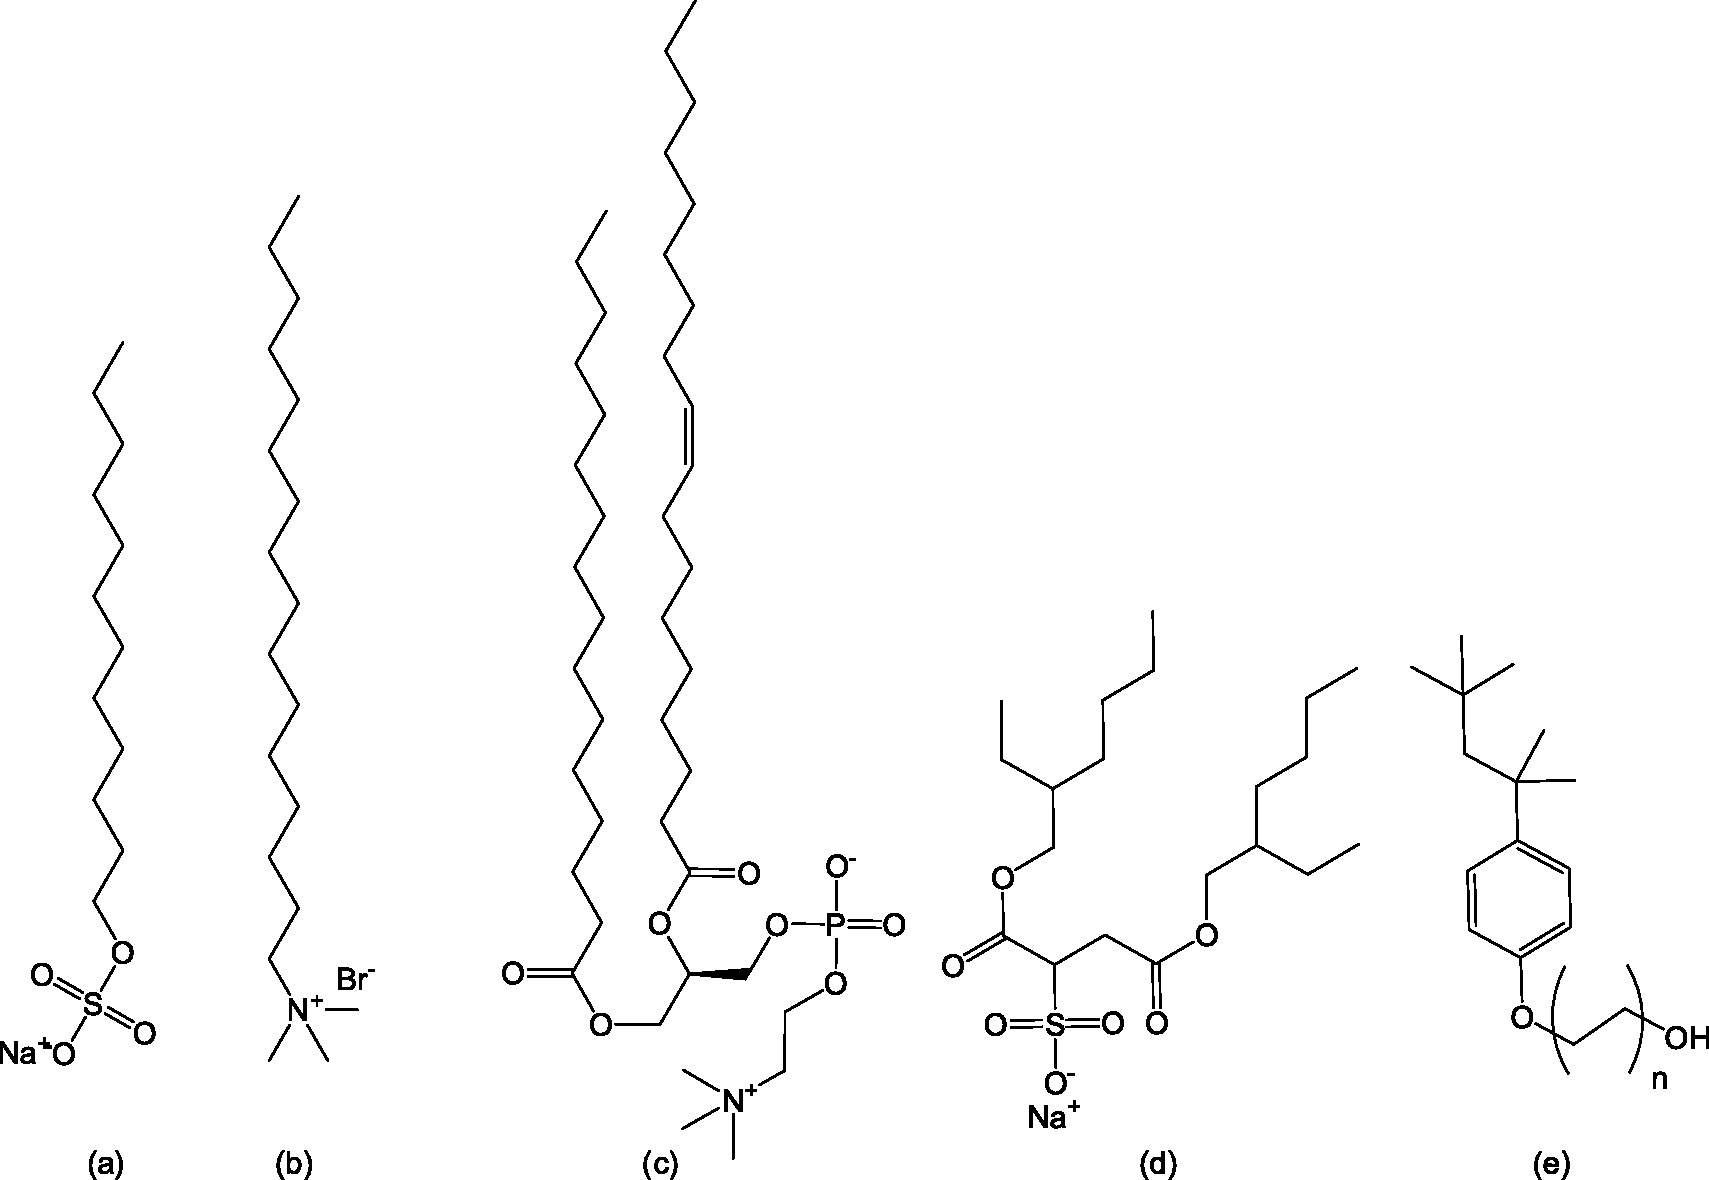
\includegraphics[width=0.7\textwidth]{./imagens/introducao/estrutura_surfactantes}
		%\caption[Estrutura de alguns surfactantes]{Estrutura de alguns surfactantes. (a) dodecilsulfato de sódio (SDS) (b) brometo de hexadeciltrimetilamônio (\CTAB) (c) 1-palmitoil-2-oleoil-3-sn-fosfatidilcolina (d) bis-(2-etilhexil) sulfosuccinato de sódio (AOT) (e) poli(etilenoglicol) p-(1,1,3,3-tetrametilbutil)-fenil éter (Triton X-100)}
		\caption{Estrutura de alguns surfactantes. (a) dodecilsulfato de sódio (SDS) (b) brometo de hexadeciltrimetilamônio (\CTAB) (c) 1-palmitoil-2-oleoil-3-sn-fosfatidilcolina (d) bis-(2-etilhexil) sulfosuccinato de sódio (AOT) (e) poli(etilenoglicol) p-(1,1,3,3-tetrametilbutil)-fenil éter (Triton X-100)}
		\label{fig:estrutura_surfactantes}
	\end{figure} \index{surfactantes!estrutura}
	
	Essa dualidade os caracteriza como anfífilos,\cite{ColloidalDomain}, do grego \emph{amphi}, ``de dois tipos'', da mesma raiz de anfíbio, e \emph{philos}, ``amigável''. As duas regiões são chamadas de região liofílica (interage bem com o solvente) e liofóbica (interage mal com o solvente). Quando o solvente é água, essas regiões são chamadas então hidrofílicas e hidrofóbicas, respectivamente, e essa será a nomenclatura adotada neste trabalho, por clareza. Dessa diferença de afinidade se origina sua atividade superficial. Por exemplo, na interface água-ar, a região hidrofílica de um surfactante pode permanecer em água, enquanto a região hidrofóbica se orienta a evitar contato com a água, no ar, como mostra a \autoref{fig:superficie_surfactante}. Isso diminui a tensão superficial \(\gamma\), que relaciona a variação da energia superficial \(G\) com a variação na área superficial \(A\),
	
	\begin{equation}
		\gamma = \left( \dfrac{\partial G}{\partial A}  \right)_{T,P,n}
		\label{eqn:tens_superficial}
	\end{equation}
	
	\begin{figure}[h]
		\centering
		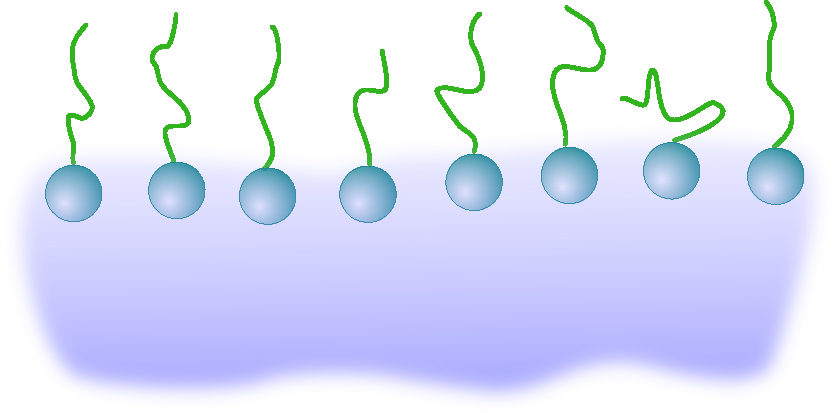
\includegraphics[width=0.7\textwidth]{./imagens/introducao/superficie_surfactante}
		\caption{Interface de água e ar, com moléculas de surfactantes direcionadas}
		\label{fig:superficie_surfactante}
	\end{figure} \index{surfactantes!atividade superficial}
		
	Devido à sua ação interfacial e a característica anfifílica, os surfactantes possuem uma grande variedade de possíveis aplicações, desde produtos básicos inventados na antiguidade, como o sabão\cite{Gibbs1939, Levey1954}, na biologia, na forma de membranas celulares e sais biliares\cite{Wennerstrom1979}, na indústria alimentícia\cite{Lauridsen1976}, na indústria química\cite{Balzer1999} e de petróleo\cite{Surfactants_petroleum}, e, inclusive, como catalizadores\cite{Minch1978a}.
	
	À medida que mais surfactante é adicionado, mais moléculas se concentram na superfície, até uma concentração limite, chamada de concentração micelar crítica (\cmc). Nesse ponto, várias propriedades do sistema mudam, como a tensão superficial, a condutividade, pressão osmótica, e outros.\cite{Lindman_livro} \index{surfactantes!concentração micelar crítica} A partir desse ponto, as moléculas de surfactante começam a formar estruturas de autoassociação, como, por exemplo, micelas esféricas, ilustradas na \autoref{fig:micela_esferica}.\cite{Lindman_livro} O termo ``micela'', do latim \emph{mica}, migalha, foi cunhado por Karl Wilhelm von Nägeli em 1858, e adotado por McBain em 1913 para descrever os agregados formados numa solução de sabão. Supostamente, seus contemporâneos não aceitaram essa ideia, dizendo ``Nonsense, McBain, Nonsense!''.\footnote{``Absurdo, McBain, Absurdo!''}\cite{Vincent2014} % todo: verificar a posição da ref e da nota de rodapé
		
	\begin{figure}[h]
		\centering
		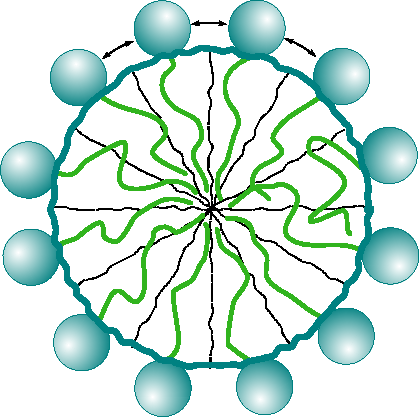
\includegraphics[width=5cm]{./imagens/introducao/micela_esferica}
		\caption{Micela esférica formada por surfactantes em água}
		\label{fig:micela_esferica}
	\end{figure}
	
	Para entender esses processos, é necessário não só observar as moléculas do surfactante, mas também as moléculas de água. A água possui interações intermoleculares muito fortes, em especial, a ligação de hidrogênio. Para maximizar o número de ligações de hidrogênio, as moléculas de água devem se organizar ao redor da cadeia hidrofóbica do surfactante, uma organização que inclusive já foi chamada de ``iceberg''\cite{FrankEvans1945}. Esse efeito, conhecido como efeito hidrofóbico\cite{Tanford1978}, é de natureza fundamentalmente entrópica. Quando as moléculas de água são liberadas, pela orientação ou formação de micelas, o ganho entrópico das moléculas de água se sobressai em relação à perda entrópica da organização das moléculas desse surfactante. Mais detalhes sobre interações intermoleculares e o efeito hidrofóbico podem ser encontradas na \autoref{sec:forcas_intermoleculares}.

	Outras estruturas de autoassociação, além de micelas esféricas, são possíveis.\cite{Lindman_livro} Micelas esféricas podem se deformar, gerando micelas elipsoidais triaxiais.\cite{Alves2017} Após isso, as micelas podem crescer unidimensionalmente, formando micelas cilíndricas. Esse crescimento pode continuar, formando micelas que possuem uma variedade de nomes na literatura, como 
	
	\begin{itemize}[noitemsep]
		\item 670 artigos\footnote{Números adquiridos pela pesquisa de \emph{wormlike} micell* no título do artigo no Web of Science, no dia 18/12/2018}: Vermiformes, \emph{wormlike}\cite{Calabrese2018, Chu2010b, Ito2016, Lin2010a, Dreiss2007},
		\item 44 artigos: gigantes, \emph{giant}\cite{Giant_Micelles, Cates2006, Messager1988a},
		\item 27 artigos: alongadas, \emph{elongated}\cite{Shikata1987, Porte1980a, Oda1999a, Makhloufi1989},
		\item 51 artigos: filiformes, \emph{threadlike}\cite{Danino1995a, Shi2014, Imai2001a,Brown1989a},
		\item 56 artigos: parecidas com polímeros, \emph{polymer-like}\cite{Appel1990, BaldelliBombelli2002a, Garamus2000},
	\end{itemize}
	
	\noindent e inclusive combinações dos termos\cite{Won1999, Georgieva2016}. Logo, uma boa pesquisa bibliográfica necessita da inclusão de todos esses termos, o que pode ser feito pelos mecanismos de busca mais comuns utilizando operadores binários como \texttt{AND} e \texttt{OR}. Os nomes mais comuns são \emph{wormlike} em inglês e \emph{gigantes} em português. As micelas gigantes são o foco deste trabalho. Uma ilustração de micelas gigantes se encontra na \autoref{fig:micela_gigante}. \index{micelas gigantes}
		
	\begin{figure}[h]
		\centering
		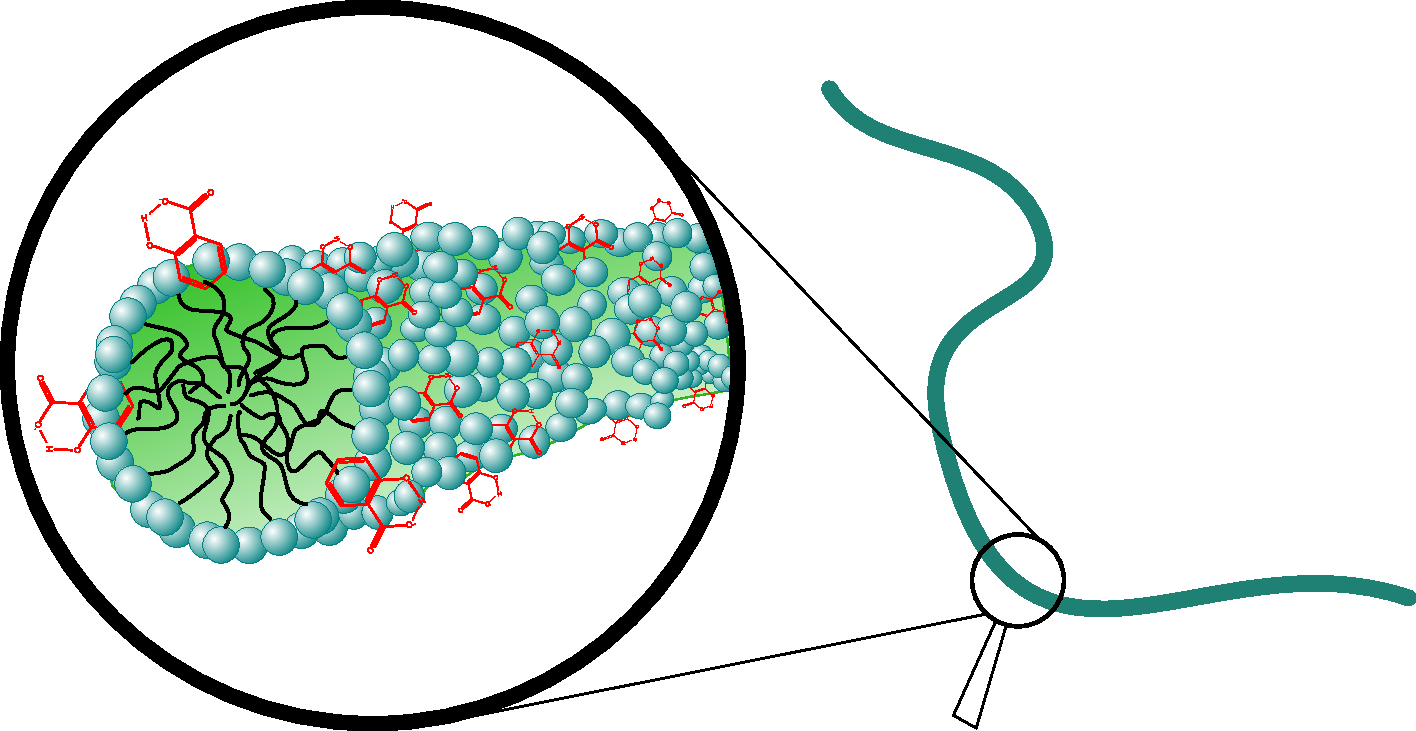
\includegraphics[width=0.7\textwidth]{./imagens/introducao/micela_gigante}
		\caption{Micela gigante formada pela interação de salicilato de sódio e brometo de hexadeciltrimetilamônio. Figura adaptada de \citeauthor{WLM_Advances}}
		\label{fig:micela_gigante}
	\end{figure}
	
	O fator que diferencia as micelas esféricas das micelas alongadas é o empacotamento das moléculas de surfactante. O parâmetro de empacotamento \(P\), definido na \autoref{eqn:param_empacot} é um parâmetro geométrico utilizado para racionalizar o empacotamento das moléculas de surfactante.\cite{Israelachvili1976c}
	
	\begin{equation}
	P = \dfrac{\dfrac{V}{l}}{a_0}
	\label{eqn:param_empacot}
	\end{equation} 
	%\index{surfactantes!parâmetro de empacotamento|see{parâmetro de empacotamento}} 
	\index{surfactantes!parâmetro de empacotamento!definição}
	
	\(V\) é o volume da cadeia hidrofóbica, \(l\) é o comprimento da mesma e \(a_0\) é a área da região polar do surfactante. A \autoref{fig:param_empacotamento} ilustra os elementos que compõem o parâmetro de empacotamento.
	
	\begin{figure}[h]
		\centering
		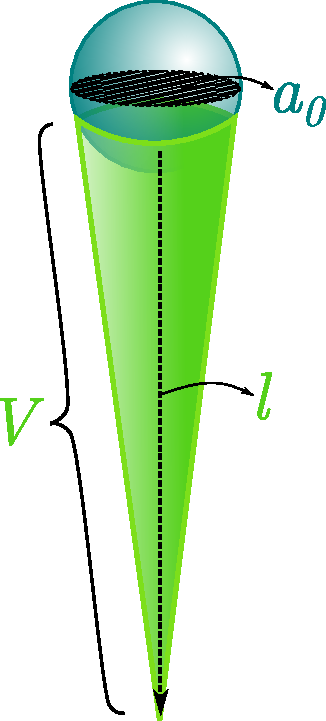
\includegraphics[width=2cm]{imagens/introducao/param_empacotamento}
		\caption{Ilustração do parâmetro de empacotamento}
		\label{fig:param_empacotamento}
	\end{figure}
	
	Esse parâmetro pode ser visualizado como uma comparação entre as áreas das bases de um cilindro, sendo uma dada por \({V}/{l}\) e a outra por \(a_0\). Quando o termo hidrofóbico é pequeno, temos praticamente um cone, e valores de \(P\) menores que \(\sfrac{1}{3}\). Como a região polar é muito grande, a estrutura de autoassociação necessariamente possuirá uma curvatura alta, o que resulta em micelas esféricas. Seguindo esse raciocínio, tanto aumentando a contribuição hidrofóbica quanto diminuindo a contribuição hidrofílica, é possível obter valores de \(\sfrac{1}{3} \leq P < \sfrac{1}{2}\). Nessa condição, são formadas micelas gigantes.
	
	Prosseguindo por essa lógica, quando as contribuições das duas regiões são equivalentes, (\(P = 1\)), as moléculas de surfactante possuem um formato cilíndrico. Nessa situação, são formadas estruturas de curvatura total zero, como lamelas.\cite{Zou2007} É possível inverter essa tendência aumentando a contribuição da parte hidrofóbica, gerando agregados com grande curvatura, mas de maneira oposta. Nesse caso, são formadas micelas reversas, cilíndricas\cite{Tung2006} ou esféricas\cite{Mackeben2001a}. \index{surfactantes!parâmetro de empacotamento} Um diagrama com várias estruturas de autoassociação possíveis se encontra em \citeauthor{Lindman_livro}.

	É possível controlar a estrutura de autoassociação controlando-se os parâmetros de \(P\). A adição de um sal inorgânico a um surfactante iônico, por exemplo, blinda as cargas da superfície micelar, diminuindo \(a_0\). Isso diminui a \cmc{} de surfactantes iônicos\cite{Sarac2009} e, com a adição de sal suficiente, pode causar a transição para micelas cilíndricas,\cite{Garamus2003a} ou até gigantes.\cite{Helgeson2010d} \index{surfactantes!blindagem da carga}
	
	De maneira similar, o aumento da cadeia hidrofóbica (\(l\)) de um surfactante induz a micelização em concentrações menores (diminui a \cmc).\cite{Bai2008, Sarac2017a} Uma alteração de \(V\) pode ser realizada tanto com o aumento do comprimento da cauda do surfactante, como também com a adição de moléculas como hidrocarbonetos e álcoois, porém o comprimento das cadeias desses aditivos afetam de maneira diferente a agregação.\cite{Bayer1986, Bielawska2013a, Kamada2014a} É importante ressaltar que o parâmetro de empacotamento se refere somente à estrutura do surfactante, mas é necessário também considerar o contexto químico do sistema, que pode alterar os parâmetros, se comparados com um surfactante isolado. \index{surfactantes!parâmetro de empacotamento}
	
	O sistema mais bem descrito na literatura para a formação de micelas gigantes é uma mistura de um surfactante catiônico, como brometo de hexadeciltrimetilamônio (\CTAB) com salicilato de sódio, NaSal.\cite{Dreiss2007} O íon \Sal{} consegue se inserir na superfície micelar, por ser planar, possuir uma região hidrofóbica e carga oposta ao surfactante, e assim diminui \(a_0\) (\autoref{fig:interacao_nasal_ctab}).\cite{Ito2014c} Além disso, as interações cátion-\(\pi\) entre o surfactante e o anel aromático\cite{Mahadevi2013a, Umeasiegbu2016} reforçam o posicionamento da molécula na paliçada micelar. \index{surfactantes!efeito de NaSal} \index{surfactantes!\CTAB}
	
	\begin{figure}[h]
		\centering
		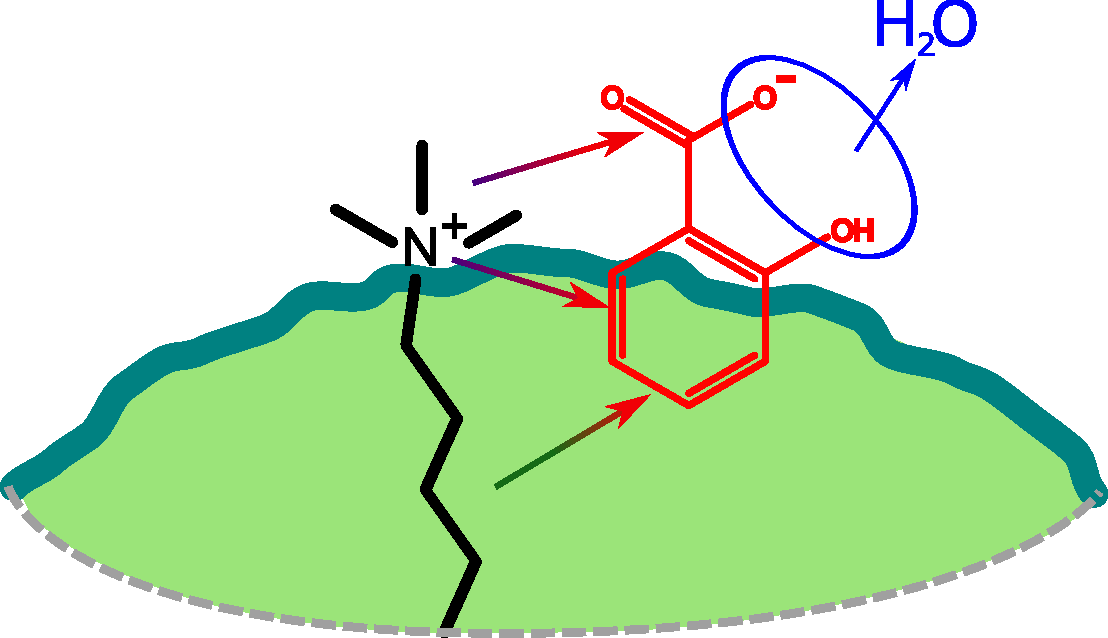
\includegraphics[width=5cm]{imagens/introducao/interacao_nasal_ctab}
		\caption{Interação da molécula de salicilato com um surfactante catiônico e com o solvente, na paliçada micelar.}
		\label{fig:interacao_nasal_ctab} \index{surfactantes!efeito de NaSal}
	\end{figure}
	
	Concentrações pequenas, tanto de surfactante quanto de NaSal são capazes de induzir a formação e crescimento micelar\cite{Sarac2013, Ito2015c}, devido à grande afinidade que o salicilato possui pela paliçada. O sistema 100 \mM{} de \CTAB{} e 100 \mM{} de NaSal forma uma solução bastante viscosa, porém uma solução 100 \mM{} de \CTAB{} e 100 \mM{} de NaCl é completamente fluída, devido à baixa afinidade do íon Cl\textsuperscript{-} pela superfície micelar.\footnote{Dados do grupo não publicados} 
	
	O solvente, como já informado, possui uma papel muito importante na formação de estruturas de autoassociação. É necessário que exista uma penalidade entrópica da solvatação do surfactante suficientemente grande para que a associação ocorra. Essa penalidade é bastante alta em água, mas inexistente em solventes como hexano. Apesar de sua importância, não há muitos estudos sobre como solventes aquosos afetam a formação, crescimento e interações de micelas gigantes. Neste trabalho, será estudado o papel de misturas binárias de água com outros componentes na formação de micelas gigantes de NaSal e surfactantes catiônicos.
		
	Uma descrição mais completa sobre micelas gigantes se encontra no \autoref{chap:micelas_gigantes}.

	\chapter{Reologia}
		\section{Fundamentos} \index{reologia!fundamentos}
		
		A reologia é a área ciência que estuda o fluxo e a deformação da matéria. O termo vem do grego \emph{rheos}, fluxo, e \emph{logia}, ciência, e foi cunhado por Bingham em 1929.\cite{Bingham1929} Para causar um fluxo ou deformação, é necessário que uma força externa seja aplicada ao corpo. Reagindo à essa força, o material se comporta de tal maneira que algumas de suas características estruturais podem ser inferidas. % Isso é feito intuitivamente por qualquer pessoa, por exemplo, ao apertar uma fruta para determinar sua firmeza e assim, se ela está apropriada para consumo ou não, para desagrado do vendedor.
		% Hiris: logia se traduz melhor como ``área da ciência''. É verdade?
		
		No campo coloidal, a reologia é utilizada para estudar como os corpos coloidais estão dispostas no meio, suas interações entre si e com o meio, e como fluem mediante a força externa. Por exemplo, soluções de micelas gigantes são altamente viscosas, pois as cadeias das micelas se entrelaçam e ramificam,\cite{Rehage1991} então existe um mecanismo para oferecer resistência à força aplicada. Já soluções de micelas esféricas possuem baixa viscosidade, pois o tamanho das micelas é pequeno, e não existe esse mecanismo. A resistência se deve principalmente ao solvente, nesse caso.
		
		A viscosidade pode ser definida, de maneira pouco rigorosa, como a resistência ao fluxo de um material.\cite{Boger1989} \index{reologia!viscosidade} Então a água possui baixa viscosidade, já o mel, uma solução concentrada de açúcar, possui alta viscosidade. Porém, quando tenta-se aplicar essa definição para outros tipos de materiais, aparecem problemas. Manteiga mantém seu formato, ao contrário de mel, que sempre flui, mas é muito mais fácil passar manteiga num pedaço de pão do que mel. Já amido de milho em água aparenta ser resistente se forçado a se mover rapidamente, mas flui quando é perturbado lentamente. Qual desses três materiais seria mais viscoso? 
		
		O comportamento desses materiais depende de sua microestrutura. Manteiga é uma emulsão de água em óleo, ou seja, há gotículas de água estabilizadas pelas proteínas do leite dispersas e compactadas num meio contínuo de óleo. A quantidade dessas gotículas, e a atração inter-gotículas, é tal que há pouca mobilidade dessas fases.\cite{Hoffmann2014a} Porém, as forças entre as gotículas podem ser rompidas quando uma força externa um pouco mais forte é aplicada. Após o rompimento, o fluxo se torna fácil. Se a força for removida, as interações são reformadas e o material volta a assumir sua consistência característica.
		
		Portanto, a viscosidade da manteiga dependeu da força que estava sendo aplicada. Em forças baixas, o material aparentava ser altamente viscoso, já em forças maiores, o material aparentava ser pouco viscoso. Não existe um valor único de viscosidade que pode ser atribuído à manteiga, da mesma maneira que é feito com água. Somente é possível estabelecer viscosidades aparentes dependentes da força aplicada.\cite{Kronberg2014a}
		
		Do lado oposto à viscosidade, no campo reológico, existe a elasticidade \index{reologia!elasticidade}. Materiais elásticos, ao invés de fluir, se deformam reversivelmente. A estrutura interna desses materiais permite que energia seja armazenada em torções e distensões. Quando a força externa é removida, a energia é liberada e o material volta ao seu formato inicial. Caso a energia aplicada supere as forças que estruturam o material, por exemplo, ligações covalentes ou interações intermoleculares, o material acaba fluindo ou quebrando.\cite{Goodwin2008} Exemplos clássicos de materiais elásticos são: molas, borrachas, rochas, madeira. A constante de elasticidade é a grandeza análoga à viscosidade, para materiais elásticos. Essa constante está relacionada à força necessária para causar uma deformação no material. \index{reologia!módulo elástico}

		Retomando o exemplo anterior, em baixos valores de tensão, a manteiga conseguia se manter estruturada. Nessa região de forças bastante pequenas, a manteiga consegue armazenar energia em sua estrutura interna. De acordo com as definições apresentadas, a manteiga pode se comportar tanto como um material elástico quanto um material viscoso. Esse tipo de material recebe o nome de material viscoelástico. Em especial, a manteiga é um material plástico, que possui uma tensão máxima de resistência, chamada de \emph{yield stress}.
		
		\subsection{Número de Deborah} \index{reologia!Número de Deborah}
		
		É possível relacionar materiais viscosos, elásticos e viscoelásticos através do número de Deborah (\autoref{eqn:Deborah})\cite{Goodwin2008}, que relaciona o tempo de relaxação do material (\(\tau_{\mathrm{rel}}\)) com o tempo de observação (\(t\)). \index{reologia!tempo de relaxação \(\tau_{\textrm{rel}}\)} 
		
		\begin{equation}
			D_e = \dfrac{\tau_{\text{rel}}}{t}
			\label{eqn:Deborah}
		\end{equation}
		
		O tempo de relaxação é, como o nome diz, o tempo que um material leva para dissipar uma tensão aplicada em si. Quando a força é aplicada por um tempo maior que o tempo de relaxação do material, a tensão é dissipada e o material flui. De maneira oposta, caso a tensão seja aplicada por um tempo bastante curto, comparativamente, não há tempo para o material perder a energia, e mantém assim o seu formato.
		
		Por exemplo, uma mola metálica resiste forças compressivas e expansivas. Porém, se comprimida ou expandida por muito tempo, os defeitos cristalinos do metal podem começar a se locomover, e a mola perde parte de suas características elásticas, um fenômeno conhecido como fluência (\emph{creep}). Logo, o material que aparentemente é sempre elástico, pode fluir, demonstrando um pouco de comportamento viscoso.\cite{Crossland1973, Schleichert2017}
				
		Água, no outro extremo, é um material que se comporta quase sempre como um líquido. Porém, assim como a mola, pode agir de maneira oposta. Se o tempo do experimento for muito rápido, como num impacto de curtíssima duração, as moléculas de água não tem tempo suficiente para se deslocar, e a água aparenta ser um sólido.\cite{Goodwin2008}
		
		Soluções de micelas gigantes combinam ambos os comportamentos elástico e viscoso.\cite{Pilpel1966, Hoffmann1982a} \index{reologia!viscoelasticidade} Isso é observado claramente no efeito de recuo (\emph{recoil}), \index{micelas gigantes!recoil@\textsl{recoil}} quando uma solução de micelas gigantes é agitada circularmente.\cite{Hoffmann1988a} Inicialmente, observa-se a solução seguindo o sentido do fluxo através das bolhas formadas pela agitação. Quando a agitação cessa, o fluxo continua por um tempo, devido à sua inércia, depois para e começa a fluir no sentido contrário (recuo), podendo até oscilar várias vezes, se a solução for bastante elástica. Isso ocorre porque as cadeias de micelas gigantes interagem entre si e se entrelaçam de tal modo que um pouco da energia da agitação é armazenada. Ao interromper a agitação, essa energia consegue ser liberada, o que ocorre no sentido oposto à agitação, então o recuo é observado. Depois do recuo, a solução para de se movimentar pois toda a energia foi dissipada. A escala de tempo para a perda de energia e para o \emph{recoil} são aproximadamente iguais, logo o número de Deborah desse fluido é próximo de 1.
		
		A correlação entre o número de Deborah e o comportamento do material pode ser resumido pela \autoref{eqn:Deborah_casos}\cite{Goodwin2008}
		
		\begin{equation}
			D_e
			\begin{cases}
				\gg 1     & \textrm{Elástico, semelhante a um sólido}      \\
				\approx 1 & \textrm{Viscoelástico} \\
				\ll 1     & \textrm{Viscoso, semelhante a um líquido}
			\end{cases}
			\label{eqn:Deborah_casos}
		\end{equation} \index{reologia!Número de Deborah|textbf}
		
		No tempo de ação típico de uma mola, seu tempo de relaxação é bastante longo, então \(D_e \gg 1\). Porém, se armazenada numa posição longe de seu estado sem tensão, em especial em temperaturas altas, a situação se inverte, e \(D_e \ll 1\), logo, a mola flui e adota um novo formato. Dessa maneira, a mola, e os outros materiais citados se comportam como materiais tanto elásticos quanto viscosos, dependendo do tempo de análise \(t\). O nome desse número vem de uma passagem bíblica, \emph{Os montes deslizaram diante do Senhor}\footnote{Juízes 5:5}. Mesmo as montanhas, que tradicionalmente não se movem, acabam deslizando mediante tempos de observação infinitos.
		
		Para um estudo mais aprofundado de reologia, é necessário estabelecer um formalismo matemático, que será feito nas seções a seguir.
		
			\subsection{Cisalhamento e curvas de fluxo} \index{reologia!cisalhamento}
			
			O cisalhamento é um tipo de movimento que ocorre no sentido do plano da amostra, perpendicular ao plano normal (\autoref{fig:cisalhamento}). A magnitude do cisalhamento \(\gamma\) é calculada a partir da altura \(z\) da amostra e o grau de deformação \(\Delta x\), como mostra a \autoref{eqn:cisalhamento}\cite{Goodwin2008}. \(\gamma\) é adimensional.
			
			\begin{equation}  
				\gamma = \frac{\Delta x}{z}
				\label{eqn:cisalhamento}
			\end{equation} \index{reologia!deformação \(\gamma\)}
			
			\begin{figure}[h]
				\centering
				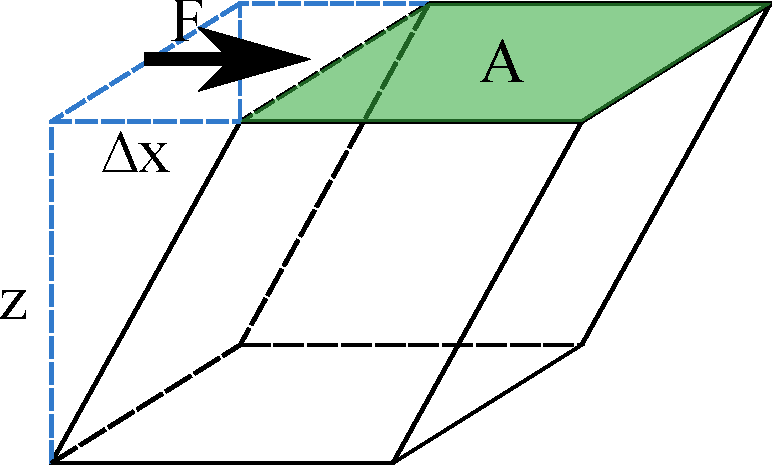
\includegraphics[width=0.5\textwidth]{imagens/reologia/cisalhamento}
				\caption{Ilustração da deformação de um material mediante a aplicação de uma força cisalhante \(F\) sobre uma área \(A\), resultando numa variação na posição de \(\Delta x\) a uma altura \(z\). Adaptado de \citeauthor{Barnes_introduction_rheology}
				}
				\label{fig:cisalhamento}
			\end{figure} 
			
			A tensão de cisalhamento \(\sigma\) é a força \(F\) necessária para aplicar um cisalhamento divido pela área de aplicação (\autoref{eqn:tensao_cisalhamento})\cite{Kronberg2014a}. A unidade usual para \(\sigma\) é Pa. Comumente, a tensão é também simbolizada por \(\tau\). \index{reologia!tensão de cisalhamento \(\sigma\)}
			
			\begin{equation}
				\sigma = \frac{F}{A}
				\label{eqn:tensao_cisalhamento}
			\end{equation}
			
			A velocidade de cisalhamento é conhecida também como taxa de cisalhamento \(\dot{\gamma}\), calculada a partir da derivada em relação ao tempo de \(\gamma\) (\autoref{eqn:taxa_cisalhamento})\cite{Kronberg2014a}. A unidade usual de \(\dot{\gamma}\) é s\menosUm. \index{reologia!taxa de cisalhamento \(\dot{\gamma}\)} Algumas referências utilizam a notação de \(\dot{\gamma}\) e outras utilizam o símbolo \(D\), mais fácil de ser digitado.\cite{Schramm1994}
			
			\begin{equation}
				\dot{\gamma} = \dfrac{\partial \gamma}{\partial t}
				\label{eqn:taxa_cisalhamento}
			\end{equation}
			
			\citeauthor{Barnes_introduction_rheology} mostram, na página 13, as taxas de cisalhamento de alguns processos habituais. Por exemplo, a drenagem de tintas pela gravidade produz taxas de cisalhamento da ordem de 10\menosUm a 10\textsuperscript{1} s\menosUm, já o ato de passar um creme na pele produz taxas da ordem de 10\textsuperscript{4} a 10\textsuperscript{5} s\menosUm.
						
			\subsection{Fluidos Newtonianos}
			
			Os fluidos Newtonianos são caracterizados por possuírem somente um valor para viscosidade \(\eta\), independente da taxa de cisalhamento, relação simbolizada pela \autoref{eqn:Newton}.\cite{Goodwin2008} Um modelo físico frequentemente utilizado para fluidos Newtonianos é o dissipador viscoso (\emph{dashpot}).\cite{Goodwin2008}
			
			\begin{equation}
				\sigma = \eta\dot{\gamma}
				\label{eqn:Newton}
			\end{equation} \index{reologia!equação de Newton} \index{reologia!viscosidade|textbf}
			
			É possível obter o valor de viscosidade de um material aplicando-se uma taxa de cisalhamento crescente e medindo a tensão necessária para manter essa taxa (modo \emph{control rate}, \emph{CR}), ou aplicando-se uma tensão e medindo-se a taxa (modo \emph{control stress}, \emph{CS}). A informação resultante desse tipo de análise se chama curva de fluxo.\cite{Schramm1994} \index{reologia!curva de fluxo}
			
			A \autoref{fig:reol_newt_exemplos} mostra curvas de fluxo simuladas para um fluido Newtoniano de viscosidade \(\eta=10\) Pa.s\menosUm.
			
			\begin{figure}[h]
				\begin{subfigure}[t]{.5\textwidth}
					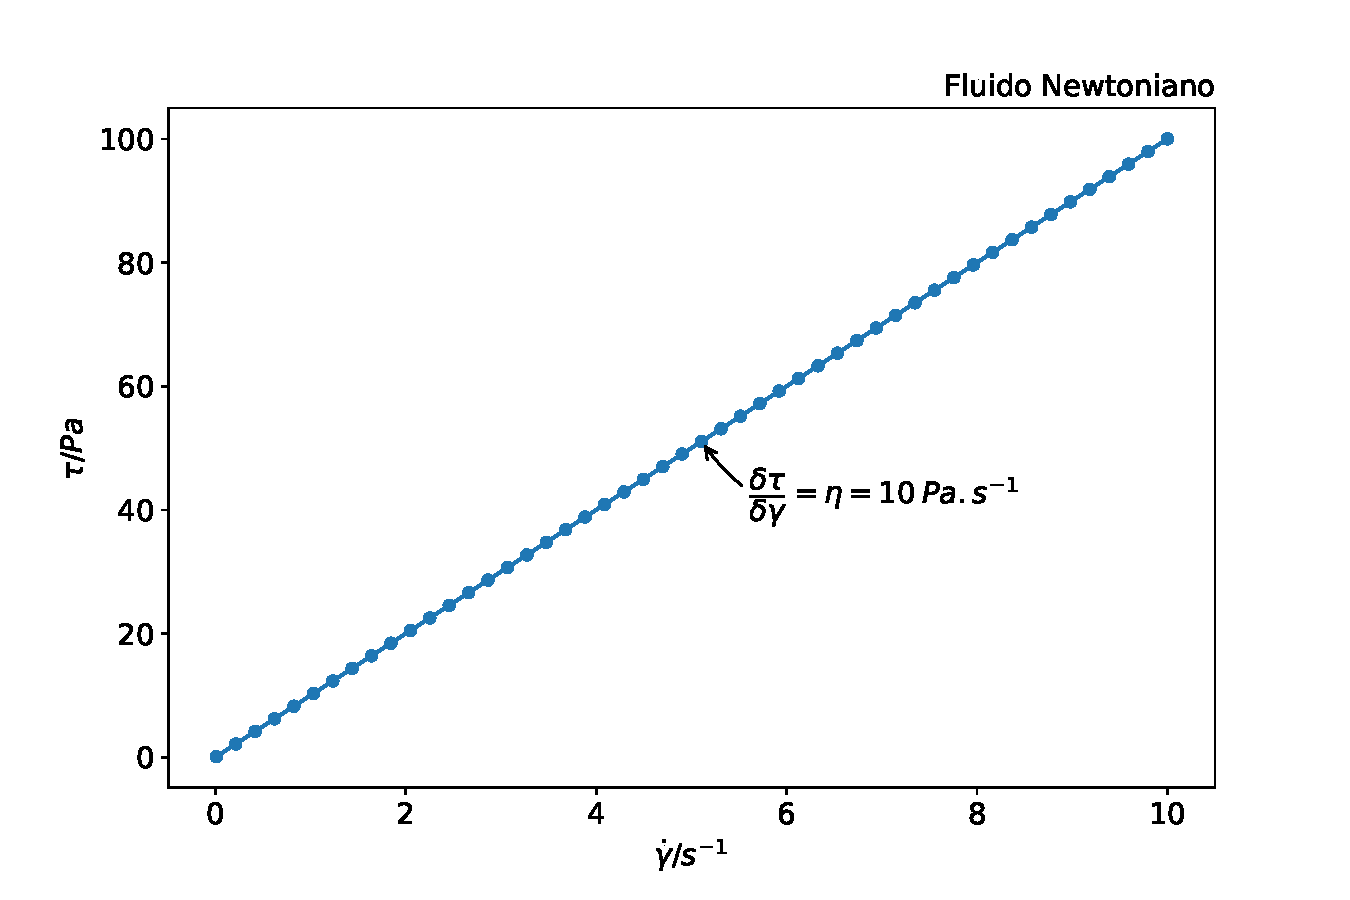
\includegraphics[width=\textwidth]{./imagens/reologia/newtoniano_exemplo_tauGP}
					\caption{\(\tau \times \dot{\gamma}\)}
					\label{fig:reol_newt_tauGP}
				\end{subfigure}%
				\begin{subfigure}[t]{.5\textwidth}
					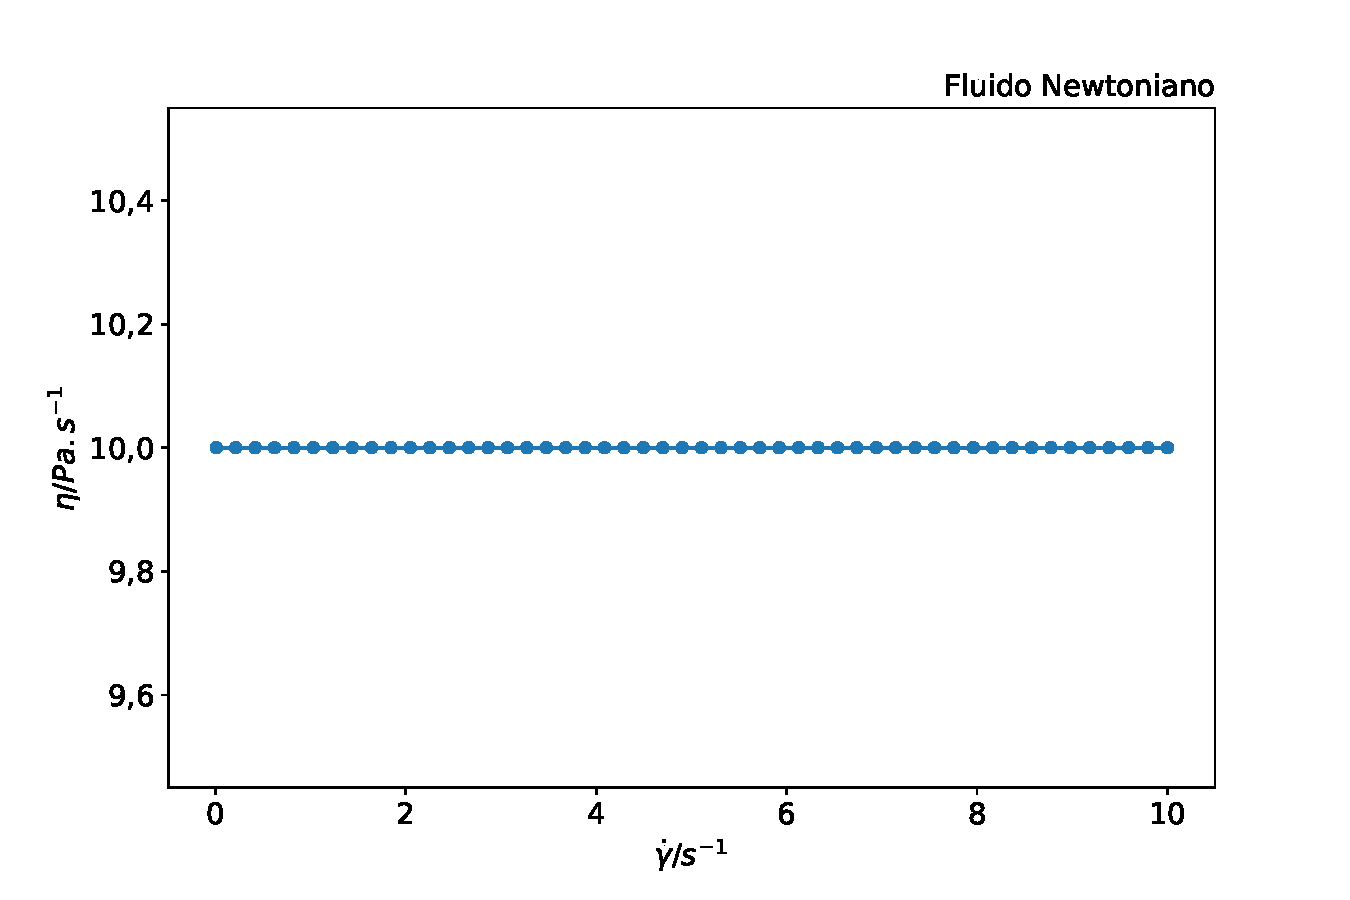
\includegraphics[width=\textwidth]{./imagens/reologia/newtoniano_exemplo_etaGP}
					\caption{\(\eta \times \dot{\gamma}\)}
					\label{fig:reol_newt_etaGP}
				\end{subfigure}
				\caption{Exemplos de curvas de fluxo. (\ref{fig:reol_newt_tauGP}) Método para obtenção da viscosidade. (\ref{fig:reol_newt_etaGP}) Dependência da viscosidade com a taxa de cisalhamento, mostrando que o valor é constante.}
				\label{fig:reol_newt_exemplos}
			\end{figure}
				
			\subsection{Sólidos Hookeanos}
			
			Sólidos Hookeanos possuem uma constante elástica \(G\) que relaciona a tensão \(\sigma\) aplicada e a deformação \(\gamma\) (\autoref{eqn:Hooke})\cite{Goodwin2008}. \index{reologia!constante elástica \(G\)}
			
			\begin{equation} 
				\sigma = G\gamma
				\label{eqn:Hooke}
			\end{equation} \index{reologia!equação de Hooke}
			
			A deformação de um sólido Hookeano pode ser tanto compressiva quando extensiva, dependendo do sinal de \(\gamma\), e consequentemente a tensão retornada possui a direção oposta da tensão aplicada inicialmente. 
			
			O modelo físico associado ao sólido Hookeano é a mola.\cite{Goodwin2008} É possível que uma mola, quando estendida demasiadamente, não retorne à sua extensão original. Isso ocorre porque a \autoref{eqn:Hooke} se aplica somente a uma região dos possíveis valores de \(\gamma\). A \autoref{fig:naohookeano_goodwinhughes} mostra o comportamento Hookeano, e não Hookeano, de uma borracha vulcanizada.
					
			\begin{figure}
				\centering
				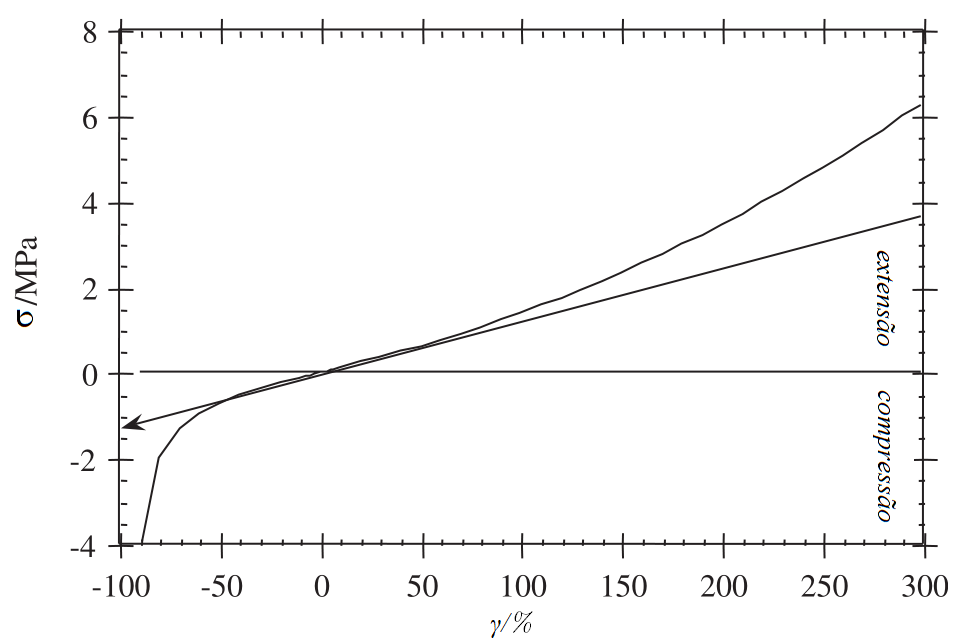
\includegraphics[width=0.7\linewidth]{imagens/artigos/nao_hookeano_goodwin_hughes}
				\caption{Tensão por extensão de cisalhamento de uma amostra de borracha vulcanizada. A região Hookeana está entre 40\% de deformação. Além disso, o comportamento da borracha desvia, e é possível que danos ocorram à estrutura. Retirado de \citeauthor{Goodwin2008}}
				\label{fig:naohookeano_goodwinhughes}
			\end{figure}

			\subsection{Fluidos não-Newtonianos} \index{reologia!fluidos não Newtonianos}
			\label{sec:teoria_fluidos_NN}
			Fluidos que não obedecem à lei de Newton (\autoref{eqn:Newton}), portanto possuem valores de viscosidade dependentes da taxa de cisalhamento, são chamados de fluidos não-Newtonianos. Dentro dessa classificação, há vários tipos de fluido, dependendo de como \(\eta\) varia com \(\dot{\gamma}\). Alguns dos tipos possíveis são:\cite{Kronberg2014a}
			
			\begin{itemize}[noitemsep]
				\item Plásticos: Viscosidade inicial é muito alta ou, teoricamente, infinita, até a tensão atingir um valor específico, chamado de tensão limite ou \emph{yield-stress}, quando o material começa a fluir. Exemplo: Metais, concreto.
				\item Pseudoplásticos ou \emph{shear-thinning}: Viscosidade alta, mas finita, em baixas taxas de cisalhamento, e decai com o aumento da taxa de cisalhamento, atingindo um valor mínimo. Exemplo: soluções de micelas gigantes, tintas.
				\item Dilatantes ou \emph{shear-thickening}: Viscosidade baixa a baixas taxas de cisalhamento, e aumenta com o aumento da taxa. Exemplo: Dispersões concentradas de amido em água.
			\end{itemize}
			
			% todo: pensar melhor sobre isso de contribuições elásticas e viscosas. O que eu escrevi aqui é o oposto do que aparece no diagrama de frequência, com a viscosidade complexa. Qual é a relação?
			
			Sob taxas de cisalhamento baixas, micelas gigantes, dependendo da concentração, podem estar emaranhadas. Isso dificulta a movimentação do solvente e da solução como um todo, resultado em uma viscosidade aparente alta. Quanto maior for o entrelaçamento das micelas, maior é a viscosidade aparente. \index{reologia!viscosidade aparente} \index{micelas gigantes!viscosidade aparente} \index{micelas gigantes!comportamento pseudoplástico} À medida que a taxa é aumentada, as micelas gigantes começam a se alinhar ao fluxo, de modo a diminuir o gradiente radial de velocidade que cada cadeia sente. Isso facilita o fluxo e diminui a estruturação que resulta no comportamento elástico, o que acaba diminuindo a viscosidade aparente.\cite{Rehage1991}
			
			Após um valor específico de taxa de cisalhamento, a viscosidade atinge um mínimo pois não há mais como aumentar o alinhamento das micelas. Nessa situação, a viscosidade aparente é predominantemente devido ao solvente, e a contribuição Newtoniana é predominante. A \autoref{fig:reol_pseudoplastico_exemplos} mostra a curva de fluxo de um material pseudoplástico.\footnote{Parâmetros: Modelo de Carreau, \(\eta_0=10\), \(\eta_{\infty}=1\), \(\dot{\gamma}_b=10\), \(n=10\).} É possível que as cadeias comecem a se estruturar, formando \emph{shear induced structures}, aumentando a viscosidade,\cite{Landazuri2013a} mas isso não foi observado neste trabalho. \index{reologia!fluidos não Newtonianos!pseudoplástico}

			\begin{figure}[h]
				\begin{subfigure}[t]{.5\textwidth}
					\includegraphics[width=\textwidth]{./imagens/reologia/pseudoplastico_tau}
					\caption{\(\sigma \times \dot{\gamma}\)}
					\label{fig:reol_pseudo_tauGP}
				\end{subfigure}%
				\begin{subfigure}[t]{.5\textwidth}
					\includegraphics[width=\textwidth]{./imagens/reologia/pseudoplastico_eta}
					\caption{\(\eta \times \dot{\gamma}\)}
					\label{fig:reol_pseudo_etaGP}
				\end{subfigure}
				\caption{Exemplos de curvas de fluxo de um fluido pseudoplástico. (\ref{fig:reol_newt_tauGP}) Tensão aplicada em função da taxa de cisalhamento. (\ref{fig:reol_newt_etaGP}) Derivada de (\ref{fig:reol_newt_tauGP}) em função da taxa de cisalhamento.}
				\label{fig:reol_pseudoplastico_exemplos}
			\end{figure} \index{reologia!curva de fluxo}
			
			No entanto, as curvas de fluxo são frequentemente plotadas na escala log-log. Nesse tipo de gráfico (\autoref{fig:reol_pseudoplastico_loglog}), é possível observar a região com viscosidade constante em baixas taxas de cisalhamento, chamada de platô Newtoniano, devido à sua constância. A viscosidade determinada nessa condição é chamada de viscosidade no repouso (\emph{zero-shear viscosity}), \(\eta_0\).\cite{Kronberg2014a}
			
			\begin{figure}[h]
				\centering
				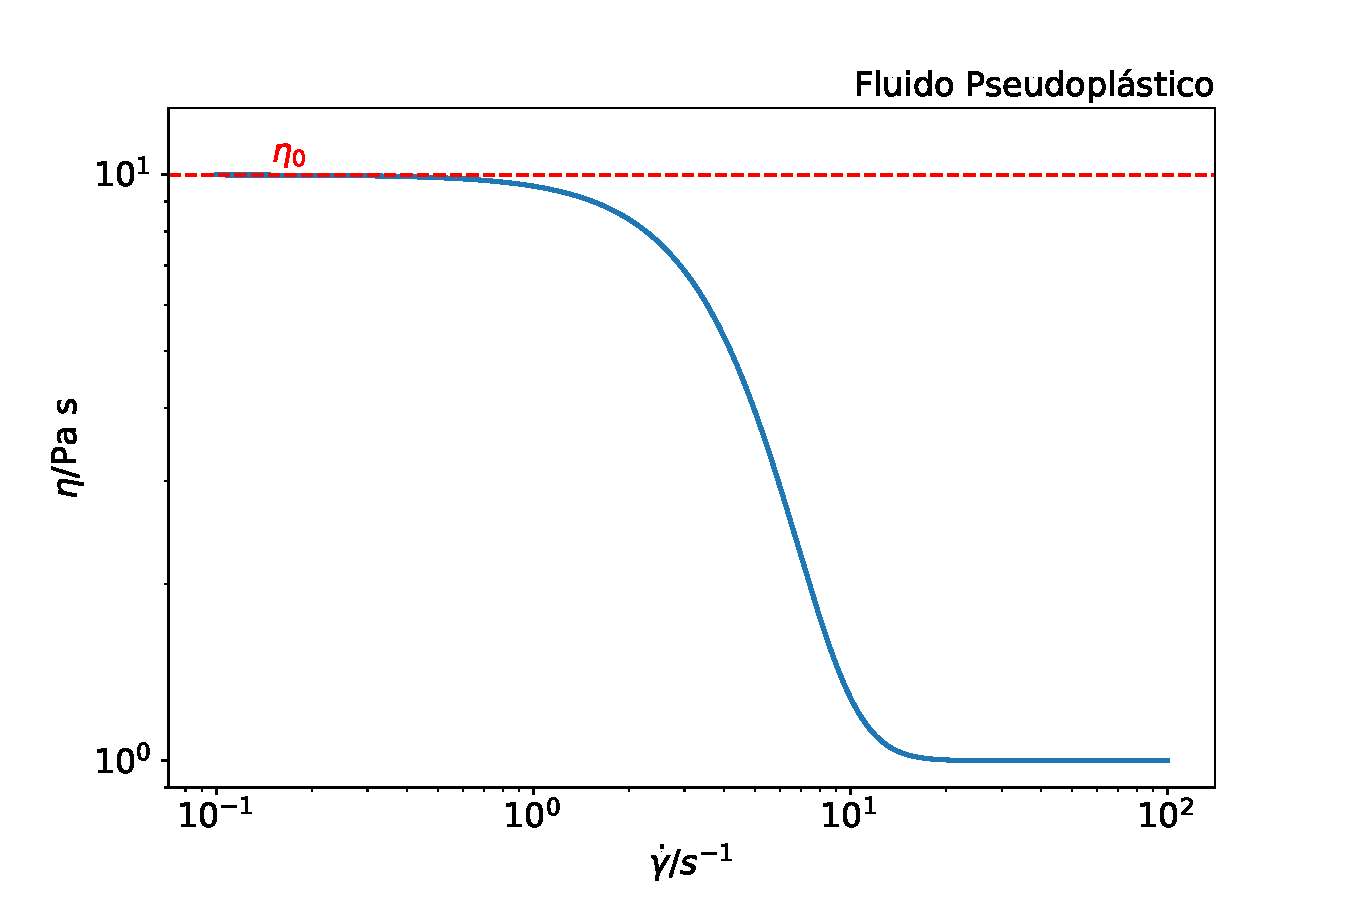
\includegraphics[width=0.7\textwidth]{./imagens/reologia/Pseudoplastico_loglog}
				\caption{Curva de fluxo de um fluído pseudoplástico na escala log-log, mostrando o valor da viscosidade no repouso, \(\eta_0\).}
				\label{fig:reol_pseudoplastico_loglog}
			\end{figure}
		
			Para obter o valor da viscosidade no repouso, é possível tanto realizar um ajuste linear da região inicial na escala log-log, ou ajustar um modelo à curva, como o modelo de Cross, Carreau e Carreau-Yasuda.
			
			\subsection{Modelagem de curvas de fluxo}
			\label{sec:modelagem_curva_fluxo}
			Dos modelos existentes na literatura, aqui serão descritos os modelos de \emph{Carreau-Yasuda} (\ref{eqn:AP_CarreauYasuda})\cite{Kwiatkowski2016a}, \emph{Carreau} (\autoref{eqn:AP_Carreau})\cite{Boger1989} e \emph{Cross} (\autoref{eqn:AP_Cross})\cite{Boger1989}. Além disso, é possível estimar a viscosidade no repouso por um ajuste linear da região de baixas taxas de cisalhamento. Os modelos correlacionam a taxa de cisalhamento (\(\dot{\gamma}\), variável independente) à viscosidade (\(\eta\), variável dependente) utilizando alguns parâmetros.
			
			\begin{equation}
			\eta = \eta_{\infty} + \frac{\eta_0 - \eta_{\infty}}{\left[  1 + \left(  \dfrac{\dot{\gamma}}{\dot{\gamma}_b}  \right)^{a}  \right]^{\frac{ \left(  n - 1  \right) }{a}}}
			\label{eqn:AP_CarreauYasuda}
			\end{equation}
			
			\begin{equation}
			\eta = \eta_{\infty} + \frac{\eta_0 - \eta_{\infty}}{\left[  1 + \left(  \dfrac{\dot{\gamma}}{\dot{\gamma}_b}  \right)^{2}  \right]^{\frac{n}{2}}}
			\label{eqn:AP_Carreau}
			\end{equation}
			
			\begin{equation}
			\eta = \eta_{\infty} + \frac{\eta_0 - \eta_{\infty}}{1 + \left(  \dfrac{\dot{\gamma}}{\dot{\gamma}_b}  \right)^{n}}
			\label{eqn:AP_Cross}
			\end{equation}
			
			O modelo linear considera somente valores de viscosidade em \(\dot{\gamma}\) próximos de zero, ou seja, \(\eta = \eta_0 + 0 \times \dot{\gamma}\).
			
			A definição dos parâmetros se encontra na \autoref{tab:params_pseudoplasticos}.\cite{WLM_Advances}:
			
			\begin{table}[h]
				\IBGEtab{%
					\caption{Parâmetros dos modelos de fluidos pseudoplásticos}
					\label{tab:params_pseudoplasticos}
				}%
				{%
					\begin{tabular}{c c p{9cm}}
						\toprule
						Parâmetro      & Unidade   & Significado                                                       \\ \midrule
						\(\eta_0\)     & Pa.s      & Viscosidade no repouso*                                           \\
						\(\eta_{\infty}\)  & Pa.s      & Viscosidade no infinito                                           \\
						\(n\)        & --        & Inclinação da região de decaimento de viscosidade, índice da pseudoplasticidade                 \\
						\(\dot{\gamma}_b\) & s\menosUm & \(\dot{\gamma}\) de início da região de decaimento de viscosidade \\ \midrule
						\(a\)        & --        & curvatura               \\ \bottomrule
					\end{tabular}%
				}{}
			\end{table}
			
			A \autoref{fig:reologia_modelos} exemplifica os modelos de Carreau e Cross e como os parâmetros afetam o formato das curvas. Note que a escala dos eixos é logarítmica. Vemos que, essencialmente, ambas as curvas possuem formatos muito semelhantes, com os parâmetros escolhidos. A escolha de um modelo depende da qualidade dos dados e do desejo do experimentalista.
			
			\begin{figure}[h]
				\begin{subfigure}[t]{0.5\textwidth}
					\centering
					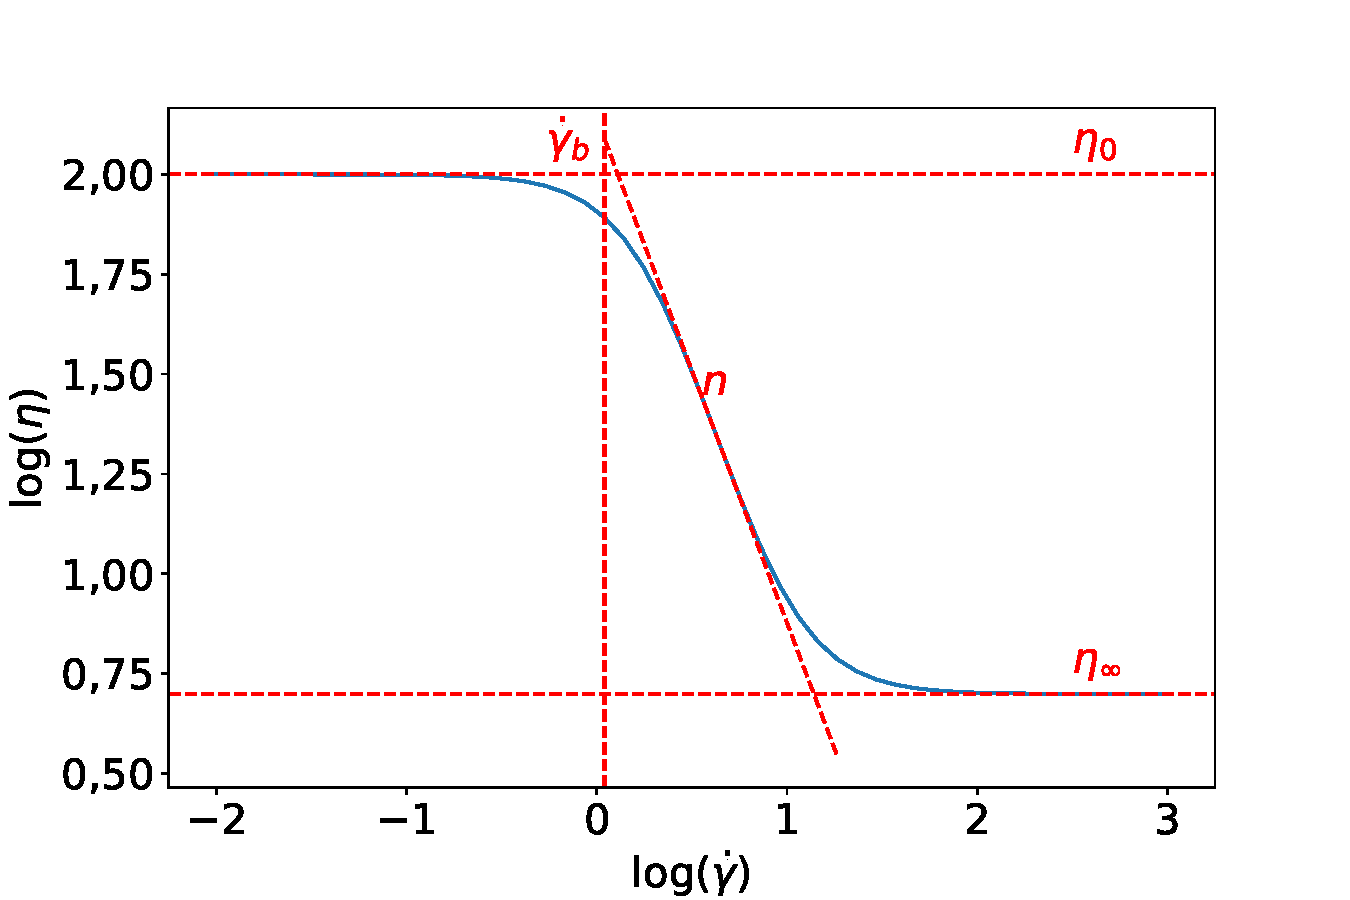
\includegraphics[width=\textwidth]{./imagens/reologia/Carreau}
					\caption{Modelo de Carreau}
					\label{fig:reologia_modelo_carreau}
				\end{subfigure}%
				\begin{subfigure}[t]{0.5\textwidth}
					\centering
					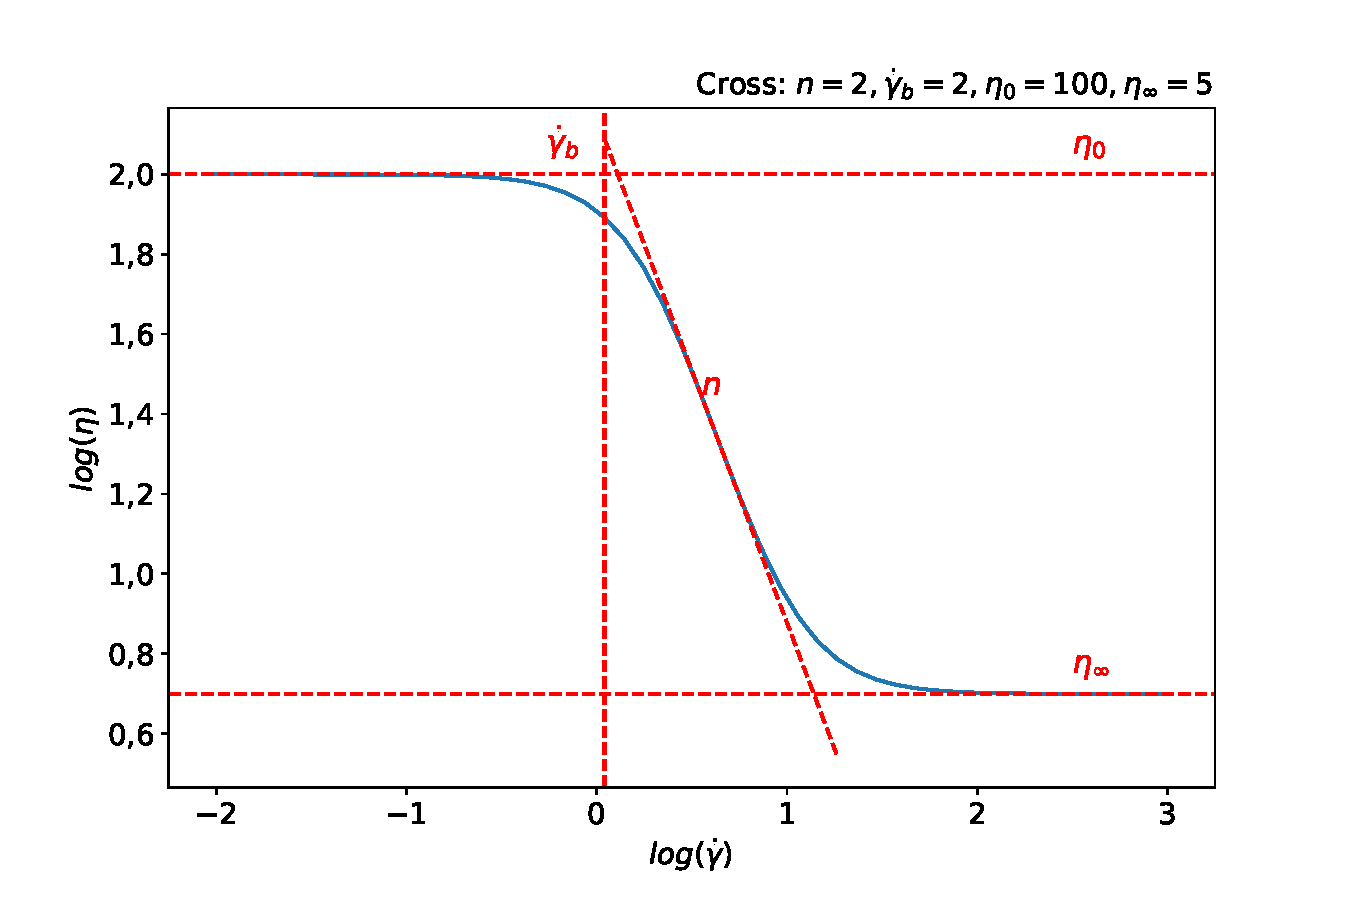
\includegraphics[width=\textwidth]{./imagens/reologia/Cross}
					\caption{Modelo de Cross}
					\label{fig:reologia_modelo_cross}
				\end{subfigure}
				\caption{Exemplos de curvas de fluxo descritas pelos modelos de Carreau e Cross. Para este exemplo, os parâmetros de ambas as curvas são: \(n=2\), \(\dot{\gamma}_b=2\) s\menosUm, \(\eta_0=100\) Pa.s, \(\eta_{\infty}=5\) Pa.s}
				\label{fig:reologia_modelos}
			
			\end{figure}
			
			Como visto nesta seção, o cisalhamento induz a alteração na estrutura dos materiais, um aumento em \(\sigma\) pode resultar num aumento não proporcional de \(\gamma\). Isso significa que o sistema está fora do regime linear. Outro tipo de experimento reológico, a reologia oscilatória, é tipicamente estudada no regime viscoelástico linear, e será descrita a seguir.\cite{Goodwin2008}
		\FloatBarrier

		\section{Reologia oscilatória} 
			\subsection{Princípios e aquisição de dados} \index{reologia!oscilatória!fundamentos}
			
			As análises oscilatórias podem ser utilizadas para obter informações reológicas mais completas sobre um material. Variando-se a frequência de perturbação, é possível obter o espectro mecânico do material, onde se observam as contribuições elástica e viscosa em função da frequência de perturbação mecânica.\cite{Goodwin2008} As derivações nesta seção se baseiam em \citeauthor{Lyklema_rheology}.
			
			Ao material, é aplicada uma deformação \(\gamma\) que varia com o tempo de acordo com
			
			\begin{equation}
				\gamma(t)=\gamma_0\cos(\omega t)
				\label{eqn:osc_gamma_t}
			\end{equation}
			
			\noindent onde \(\gamma_0\) é a deformação máxima e \(\omega\) é a frequência de perturbação. As deformações aplicadas ao material devem ser tais que não ocorra desestruturação do mesmo, isto é, o sistema deve permanecer no regime de viscoelasticidade linear. Por exemplo, uma deformação muito grande pode causar a desestruturação permanente do material, como a quebra de ligações químicas de um polímero, o que altera irreversivelmente as suas características reológicas. Por esse motivo, é necessário modular também a tensão aplicada.
			
			Um material elástico responde à deformação imediatamente com uma força no sentido oposto ao sentido da deformação. Já materiais viscosos respondem à deformação quando há uma mudança na direção, ou seja, a resposta desses materiais é totalmente defasada em relação à aplicação da deformação. Já materiais viscoelásticos, por terem componentes de ambos os tipos, possuem uma defasagem intermediária. O grau dessa defasagem é proporcional ao grau de comportamento elástico e viscoso. Levando isso em consideração, a tensão \(\sigma\)  é expressa de acordo com
			
			\begin{equation}
				\sigma = \sigma_0\cos(\omega t - \theta)
				\label{eqn:osc_tau_t}
			\end{equation} \index{reologia!oscilatória!ângulo de defasagem \(\theta\)}
			
			\noindent onde \(\sigma_0\) é a tensão máxima (determinada no experimento oscilatório de varredura de amplitude) e \(\theta\) é o ângulo de defasagem.
			
			As expressões \ref{eqn:osc_gamma_t} e \ref{eqn:osc_tau_t} podem ser reescritas utilizando a relação de Euler, \autoref{eqn:Euler}, resultando nas expressões \ref{eqn:osc_gamma_im} e \ref{eqn:osc_tau_im}, onde utilizou-se um acento circunflexo para diferenciar as expressões. Essa transformação facilita a manipulação matemática.
			
			\begin{equation}
				e^{ix} = \cos(x) + i\sin(x)
				\label{eqn:Euler}
			\end{equation} %\index{reologia!oscilatória!dedução G' e G''}
			
			\begin{equation}
				\hat{\gamma} = \gamma_0 e^{i\omega t}
				\label{eqn:osc_gamma_im}
			\end{equation}
			
			\begin{equation}
				\hat{\sigma} = \sigma_0 e^{i(\omega t - \theta)}
				\label{eqn:osc_tau_im}
			\end{equation}
			
			A partir dessas relações, é possível utilizar a equação de Hooke (\autoref{eqn:Hooke}) para encontrar o módulo elástico do material, na notação imaginária, \(\hat{G}\),
			
			\begin{equation}
				\hat{\sigma} = \hat{G}\hat{\gamma} \to \hat{G} = \dfrac{\hat{\sigma}}{\hat{\gamma}}    \to 
				\hat{G} = \dfrac{\sigma_0}{\gamma_0} \dfrac{e^{i(\omega t - \theta)}}{e^{i\omega t}} \to
				\hat{G} = \dfrac{\sigma_0}{\gamma_0} e^{-i\theta}
				\label{eqn:osc_transform_G}
			\end{equation}
			
			Utilizando-se a equação de Euler novamente, mas voltando para o domínio dos senos e cossenos, obtemos
			
			\begin{equation}
				\hat{G} = \dfrac{\sigma_0}{\gamma_0} \left( \cos(\theta) + i\sin(\theta) \right)
				\label{eqn:osc_volta_senos_G}
			\end{equation}
			
			Nessa equação, o módulo total \(\hat{G}\) foi dividido em dois termos, um em fase à deformação \(\cos(\theta)\) e outro 90° fora de fase, \(\sin(\theta)\). Esses dois termos são diretamente relacionáveis às componentes elástica e viscosa de um material. Dessa maneira, é possível separar o módulo total complexo \(\hat{G}\) em dois módulos (\autoref{eqn:osc_G_complexo}), o módulo elástico, G' (\autoref{eqn:osc_g1linha}), e o módulo viscoso, G'' (\autoref{eqn:osc_g2linha}).
			
			\begin{equation}
				\hat{G} = G' + iG''
				\label{eqn:osc_G_complexo}
			\end{equation}
			
			\begin{equation} 
				G' = \dfrac{\sigma_0}{\gamma_0} \cos(\theta)
				\label{eqn:osc_g1linha}
			\end{equation} \index{reologia!oscilatória!G'}
			
			\begin{equation} 
				G'' = \dfrac{\sigma_0}{\gamma_0} \sin(\theta)
				\label{eqn:osc_g2linha}
			\end{equation} \index{reologia!oscilatória!G''}
			
			Portanto, para conseguir separar os valores dos módulos \(G'\) e \(G''\), o reômetro necessita medir o módulo total e o ângulo de defasagem, sendo possível assim separar os componentes. Vale notar que a tangente do ângulo de defasagem é a relação \(G''/G'\),
			
			\index{módulo elástico G'|see {reologia}}
			\index{módulo viscoso G''|see {reologia}}
			
			\begin{equation}
				\tan(\theta) = \dfrac{\sin(\theta)}{\cos(\theta)} = \dfrac{G''}{G'}
				\label{eqn:osc_tan_teta}
			\end{equation}
	
			E também, é possível definir o módulo complexo \(G^*\), um módulo do módulo,
			
			\begin{equation}
				| G^* (\omega) | = \dfrac{\sigma_0}{\gamma_0} = \sqrt{\left( G' \right)^2 + \left( G'' \right)^2}
				\label{eqn:modulo_complexo}
			\end{equation}
			\index{reologia!oscilatória!módulo complexo \(G^*\)}
			
			Logo, \(\hat{G} = |G^*| e^{i\theta}\), \(G' = |G^*|\cos \theta\) e \(G'' = |G^*|\sin \theta\). Além disso, é possível definir a viscosidade complexa como função dos parâmetros G' e G'', \autoref{eqn:visc_complexa}.
			
			\begin{equation} 
			| \eta^* | = \dfrac{ |G^*| } {\omega}
			\label{eqn:visc_complexa}
			\end{equation}
			\index{reologia!oscilatória!viscosidade complexa \(\eta^*\)}
			
			A viscosidade complexa possui uma correlação direta com a viscosidade dinâmica, da curva de fluxo, em valores iguais de frequência de oscilação e taxa de cisalhamento. Essa regra é conhecida como regra de Cox-Merz.\cite{Merz1958, Manero2002a} 
			\index{reologia!regra de Cox Merz}
			
			A \autoref{fig:osc_simulacoes} mostra uma série de simulações das equações apresentadas. A deformação em função do tempo foi calculada para materiais com ângulos de defasagem \(\theta\) diferentes. \(\theta\) foi aumentado gradativamente de 0° para 90°, ou seja, o material estudado foi se tornando gradativamente mais viscoso.

			\begin{figure}[h]
				\begin{subfigure}[t]{0.3\textwidth}
					\centering
					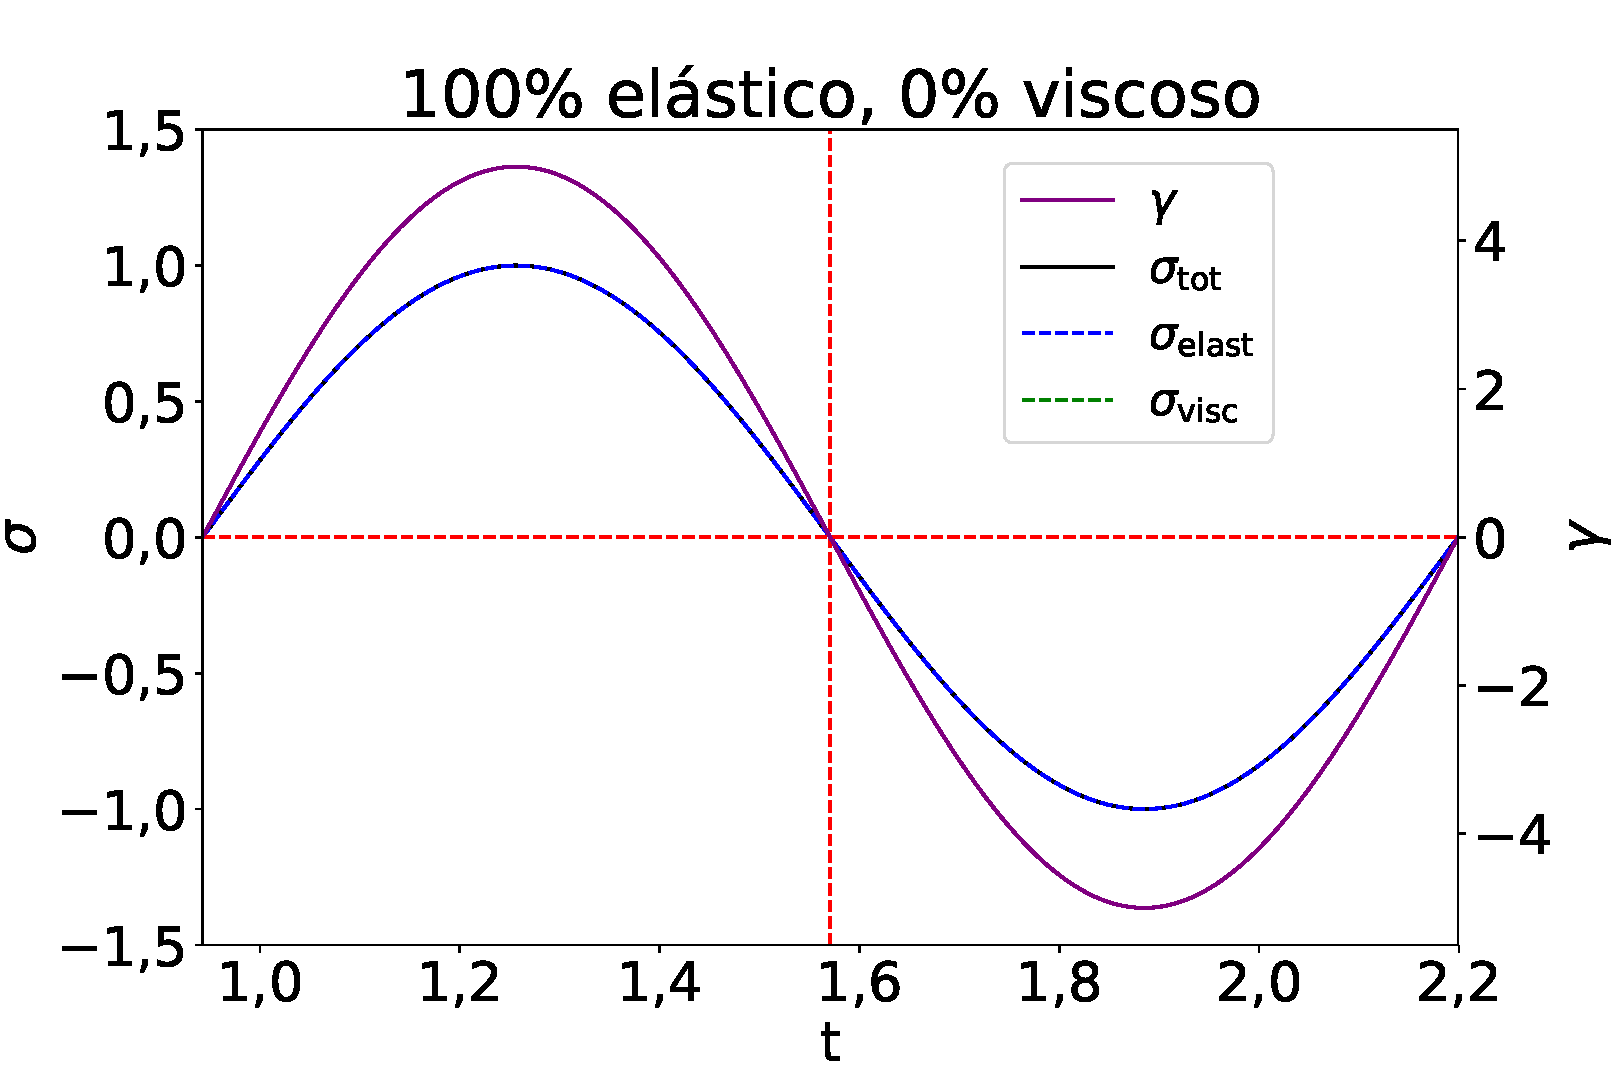
\includegraphics[width=\textwidth]{./imagens/reologia/Simulacao_visc_0}
					\caption{\(\theta=0°\)}
					\label{fig:osc_sim0}
				\end{subfigure}%
				\begin{subfigure}[t]{0.3\textwidth}
					\centering
					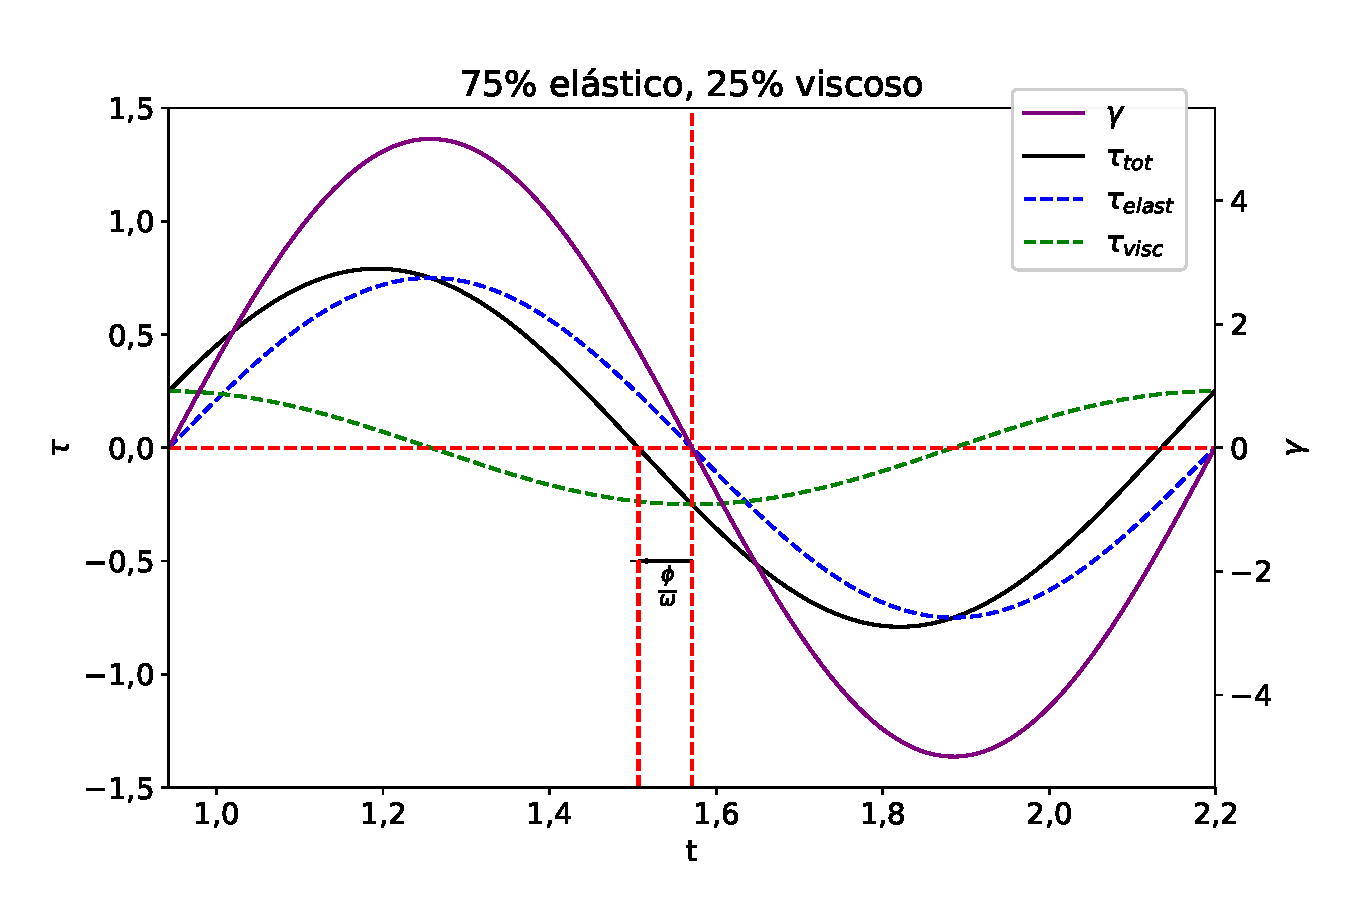
\includegraphics[width=\textwidth]{./imagens/reologia/Simulacao_visc_25}
					\caption{\(\theta=18°\)}
					\label{fig:osc_sim25}
				\end{subfigure}%
				\begin{subfigure}[t]{0.3\textwidth}
					\centering
					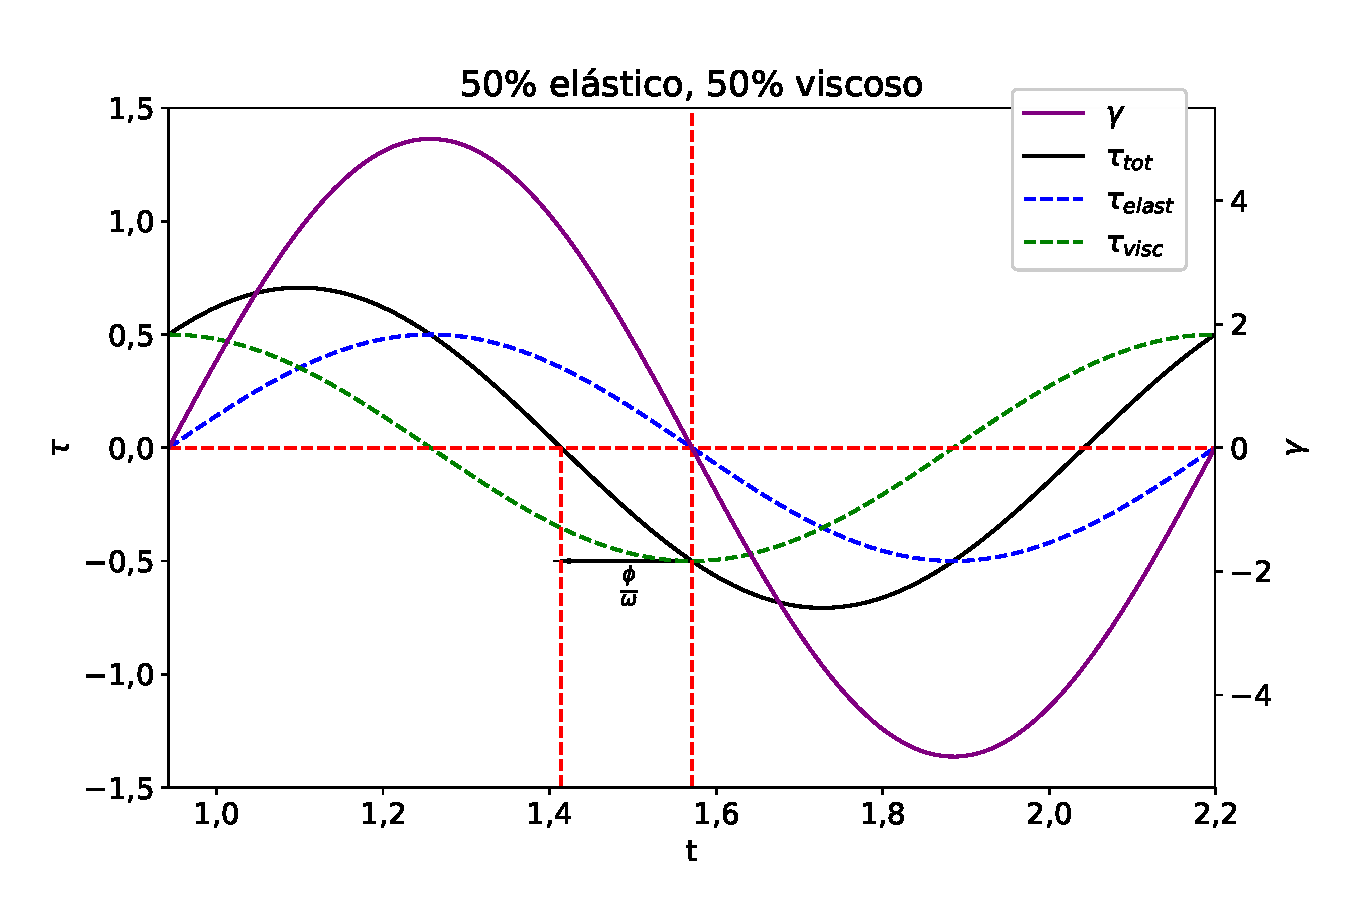
\includegraphics[width=\textwidth]{./imagens/reologia/Simulacao_visc_50}
					\caption{\(\theta=45°\)}
					\label{fig:osc_sim50}
				\end{subfigure}
			
				\hspace{2.5cm} \begin{subfigure}[t]{0.3\textwidth}
					\centering
					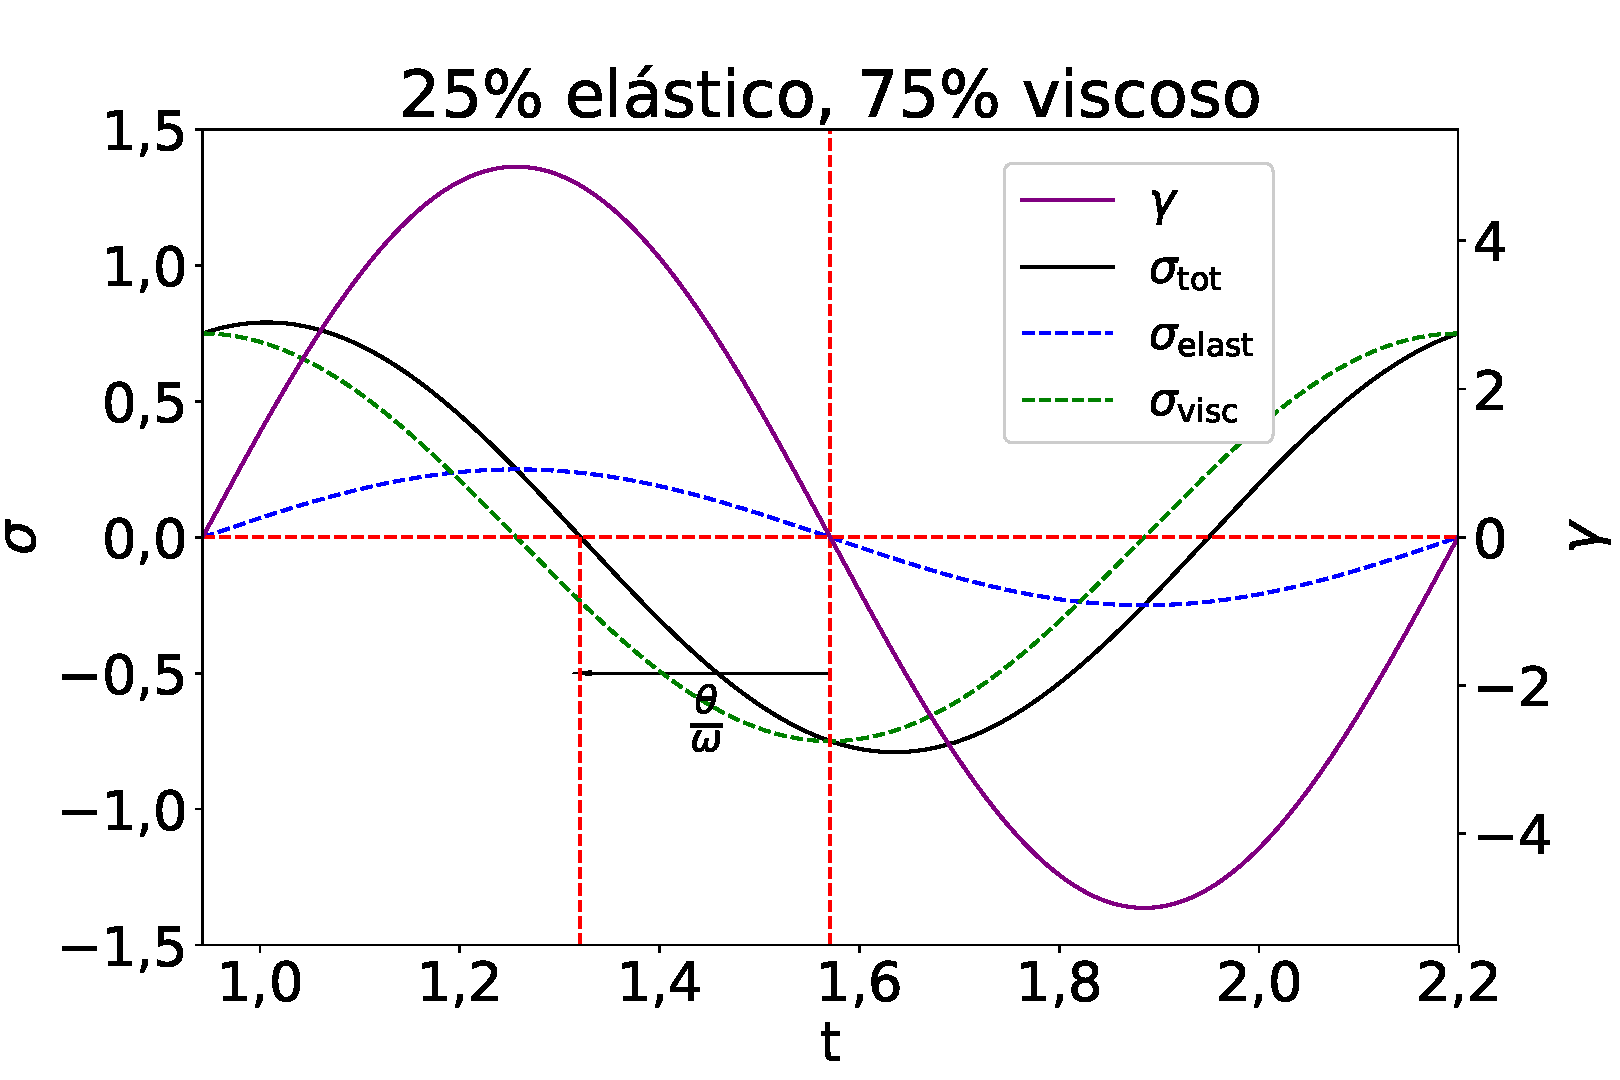
\includegraphics[width=\textwidth]{./imagens/reologia/Simulacao_visc_75}
					\caption{\(\theta=72°\)}
					\label{fig:osc_sim75}
				\end{subfigure}%
				\begin{subfigure}[t]{0.3\textwidth}
					\centering
					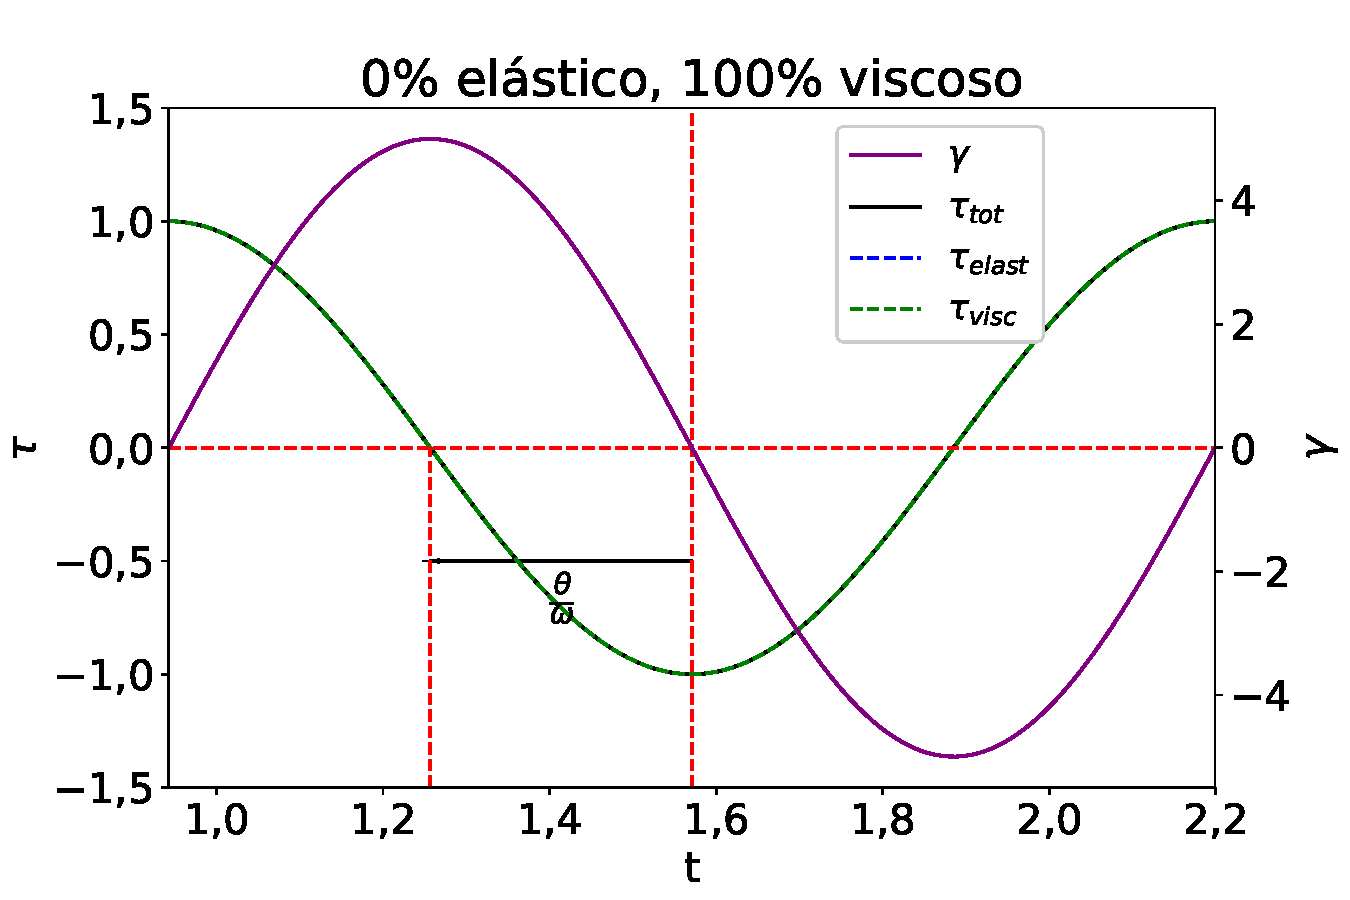
\includegraphics[width=\textwidth]{./imagens/reologia/Simulacao_visc_100}
					\caption{\(\theta=90°\)}
					\label{fig:osc_sim100}
				\end{subfigure}%
%				\begin{subfigure}[t]{0.3\textwidth}
%					\centering
%					\includegraphics[width=\textwidth]{}
%					\label{fig:}
%				\end{subfigure}
			\caption{Simulações do comportamento de um fluido sob cisalhamento cossenoidal. As imagens mostram a deformação \(\gamma\) e a tensão total \(\sigma\) de resposta, em função do tempo. A tensão também foi decomposta em suas componentes elástica e viscosa. No título de cada gráfico está a contribuição, em porcentagem, de cada componente do material. O ângulo de defasagem está ilustrado na legenda de cada subfigura.}
			\label{fig:osc_simulacoes}
			\end{figure} 
			
			\FloatBarrier
			
			\subsection{Modelo de Maxwell} \index{reologia!Modelos!Maxwell}
			\label{sec:modelo_maxwell}
			O modelo de Maxwell é construído juntando-se um elemento elástico (mola) e um elemento viscoso (dissipador), ideais, em série. A \autoref{fig:ilust_modelo_maxwell} ilustra essa construção.
			
			\begin{figure}[h]
				\centering
				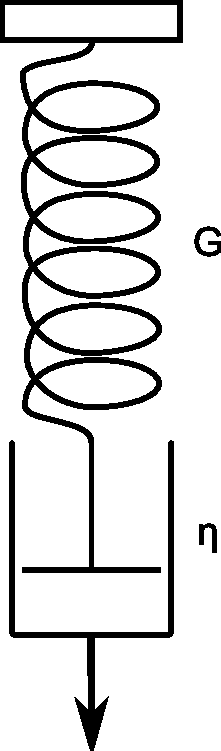
\includegraphics[width=1.5cm]{./imagens/reologia/maxwell_mola_dissipador}
				\caption{Modelo de Maxwell: Mola com constante elástica \(G\) e dissipador com constante viscosa \(\eta\) em série}
				\label{fig:ilust_modelo_maxwell}
			\end{figure}

			 É possível expressar a taxa de cisalhamento do modelo de Maxwell como a soma das taxas de cisalhamento dos elementos individuais,
			 
			\begin{equation}
				\dot{\gamma}_{\textrm{total}} =  \dot{\gamma}_{\textrm{viscoso}} + \dot{\gamma}_{\textrm{elástico}} \to
				\dfrac{\mathrm{d}\gamma}{\mathrm{d}t} = \dfrac{1}{\eta}\sigma + \dfrac{1}{G}\dfrac{\mathrm{d}\sigma}{\mathrm{d}t}
				\label{eqn:Maxwell_soma}
			\end{equation}
			
			Para uma deformação constante, \(\frac{\mathrm{d}\gamma}{\mathrm{d}t}=0\), a \autoref{eqn:Maxwell_soma} se torna uma equação diferencial,
			
			\begin{equation}
				\dfrac{1}{\eta}\sigma + \dfrac{1}{G}\dfrac{d\sigma}{dt} = 0
				\label{eqn:Maxwell_diferencial}
			\end{equation}
			
			\noindent cuja solução é 
			
			\begin{equation}
				\sigma(t) = \sigma_0 \exp \left( -\dfrac{G}{\eta}t \right)
				\label{eqn:Maxwell_dif_resolvida}
			\end{equation}
			
			O termo exponencial na \autoref{eqn:Maxwell_dif_resolvida} possui unidade de tempo e é a relação entre as componentes elástica e viscosa do material. Essa relação recebe o nome de tempo de relaxação, \(\tau_{\mathrm{rel}}\)
			
			\begin{equation}
				\sigma(t) = \sigma_0 \exp \left(\dfrac{-t}{\tau_{\textrm{rel}}}\right)
				\label{eqn:Maxwell_tempo_rel_def}
			\end{equation}
		
			O tempo de relaxação é o tempo de decaimento de \(\sigma\) para \(\sfrac{1}{e}\) do valor inicial. É interessante notar que em tempos pequenos, relativos a \(\tau_{\mathrm{rel}}\), o material responde com a tensão inicial total. Essa é a resposta imediata da mola. Porém, à medida que \(t\to\tau_{\mathrm{rel}}\), a tensão começa a decair exponencialmente e depois, em \(t \gg \tau_{\mathrm{rel}}\), tende a zero. Nessa situação, o dissipador difundiu toda a energia inicial aplicada.
			
			A \autoref{eqn:Maxwell_soma} pode ser rearranjada utilizando o tempo de relaxação,
			
			\begin{equation}
				\dfrac{\mathrm{d}\gamma}{\mathrm{d}t} = \dfrac{1}{\eta}\sigma + \dfrac{1}{G}\dfrac{\mathrm{d}\sigma}{\mathrm{d}t} \to 
				\sigma = -\dfrac{\eta}{G} \dfrac{\mathrm{d}\sigma}{\mathrm{d}t} + \eta\dfrac{\mathrm{d}\gamma}{\mathrm{d}t} =
				-\tau_{\textrm{rel}} \dfrac{\mathrm{d}\sigma}{\mathrm{d}t} + \eta\dfrac{\mathrm{d}\gamma}{\mathrm{d}t}
				\label{eqn:Maxwell_inicio_g1g2}
			\end{equation}
			
			É possível substituir as expressões de tensão (\ref{eqn:osc_gamma_im}) e deformação (\ref{eqn:osc_tau_im}) na expressão \ref{eqn:Maxwell_inicio_g1g2} para obter uma expressão em função do tempo, da frequência e do ângulo de fase. Já realizando as derivações, obtemos
			
			\begin{equation}
				\sigma_0 e^{i \left( \omega t - \theta \right)} = - \tau_{\textrm{rel}} \sigma_0 i\omega e^{i \left( \omega t - \theta \right)}     +       \eta i\omega\gamma_0e^{i\omega t}
				\label{eqn:Maxwell_substituicao}
			\end{equation}
			
			Em comum a todos os termos é a constante \(e^{i\omega t}\). Dividindo ambos os lados por essa constante, agrupando os termos com \(e^{-i\theta}\) e substituindo a viscosidade por \(G\tau_{\mathrm{rel}}\), temos
			
			\begin{equation}
				\sigma_0e^{-i\theta} \left(   1 + i\omega\tau_{\textrm{rel}}  \right) = i\omega G\tau_{\textrm{rel}}\gamma_0 \to
				\sigma_0e^{-i\theta} = \dfrac{i\omega G\tau_{\textrm{rel}}\gamma_0}{\left(   1 + i\omega\tau_{\textrm{rel}}  \right)}
				\label{eqn:Maxwell_intermediario}
			\end{equation}
			
			O termo à esquerda da \autoref{eqn:Maxwell_intermediario} é similar à definição do módulo elástico complexo, \autoref{eqn:osc_transform_G}, sendo necessário somente dividir ambos os lados por \(\gamma_0\). Realizando a substituição, temos
			
			\begin{equation}
				\hat{G} = \dfrac{\sigma_0e^{-i\theta}}{\gamma_0} = \dfrac{i\omega G\tau_{\textrm{rel}}}{\left(   1 + i\omega\tau_{\textrm{rel}}  \right)}
				\label{eqn:Maxwell_complexo_antes_sep}
			\end{equation}
			
			Note a semelhança com a equação \ref{eqn:modulo_complexo}. Seguindo o princípio de que o módulo complexo \(\hat{G}\) pode ser dividido em uma parte imaginária e uma parte real, podemos realizar o mesmo com a \autoref{eqn:Maxwell_complexo_antes_sep} multiplicando-se a fração por \(\frac{\left(   1 - i\omega\tau_{\mathrm{rel}}  \right)}{\left(   1 - i\omega\tau_{\mathrm{rel}}  \right)}\),
			
			\begin{equation}
				\hat{G} = \dfrac{  i\omega G\tau_{\textrm{rel}} - i^2 \omega^2 G \tau_{\textrm{rel}}^2        }{  1 - i^2\omega^2 \tau_{\textrm{rel}}^2          }
				\label{eqn:Maxwell_complexo_antes_sep2}
			\end{equation}
			
			Separando as partes imaginárias das partes reais e substituindo \(i^2 = -1\),
			
			\begin{equation}
				\hat{G} = \dfrac{   \omega^2 G \tau_{\textrm{rel}}^2       }{  1 + \omega^2 \tau_{\textrm{rel}}^2      } + i \dfrac{   \omega G \tau_{\textrm{rel}}        }{ 1 + \omega^2 \tau_{\textrm{rel}}^2 }
				\label{eqn:Maxwell_substituido}
			\end{equation}
			
			Seguindo a \autoref{eqn:osc_G_complexo}, \(\hat{G} = G' + iG''\), podemos definir o módulo elástico de acordo com o modelo de Maxwell como:
			
			\begin{equation}
				G' = \dfrac{ G \omega^2 \tau_{\textrm{rel}}^2   }{  1 + \omega^2 \tau_{\textrm{rel}}^2      }
				\label{eqn:Maxwell_G1_def}
			\end{equation} \index{reologia!oscilatória!G'}
			
			E o módulo viscoso, G'', como:
			
			\begin{equation}
				G'' = \dfrac{  G \omega  \tau_{\textrm{rel}}        }{ 1 + \omega^2 \tau_{\textrm{rel}}^2 }
				\label{eqn:Maxwell_G2_def}
			\end{equation} \index{reologia!oscilatória!G''}
			
			Quando G' = G'', observa-se que
			
			\begin{equation}
				G' = G'' \to %
				\dfrac{{ \cancel{G}}   \left(\omega \tau_{\textrm{rel}}\right)^{\cancel{2}}   }{{\cancel{1 + \omega^2 \tau_{\textrm{rel}}^2      }}} = %
				\dfrac{ {\cancel{G}} \cancel{\omega \tau_{\textrm{rel}} }}                   {{\cancel{1 + \omega^2 \tau_{\textrm{rel}}^2      }}}    \to %
				\omega \tau_{\mathrm{rel}} = 1 \to \tau_{\mathrm{rel}} = \dfrac{1}{\omega}
				\label{eqn:cruzamento_g1_g2}			
			\end{equation}
			
			Com isso, é possível obter o tempo de relaxação de um material Maxwelliano pelo ponto de cruzamento de G' e G''. É interessante notar que a relação \(\sfrac{G''}{G'}\), que equivale a \(\tan(\theta)\) (\autoref{eqn:osc_tan_teta}), também se relaciona com o tempo de relaxação. 
			
			\begin{equation}
				\tan(\theta) = \dfrac{G''}{G'} = \dfrac{1}{\omega\tau_{\textrm{rel}}}
				\label{eqn:Maxwell_cruzamento}
			\end{equation} \index{reologia!oscilatória!ângulo de defasagem \(\theta\)} %\index{reologia!Modelos!Maxwell|textbf}
			
			Quando G' = G'', \(\tan \theta = 1\) (\autoref{fig:osc_sim50}), e temos a mesma relação que a \autoref{eqn:Maxwell_cruzamento}. Lembrando que \(\omega\) é a frequência de perturbação, e o inverso da frequência é o tempo de observação, podemos relacionar o número de Deborah com \(\tau_\mathrm{rel}\),
			
			\begin{equation}
				\dfrac{1}{\omega\tau_{\textrm{rel}}} = \dfrac{ t_{\textrm{observação}  }}{ \tau_{\textrm{rel}}  } = \dfrac{1}{D_e}
				\label{eqn:Maxwell_cruzamento_Deborah}
			\end{equation} \index{reologia!Número de Deborah}

			A reologia oscilatória geralmente é ilustrada em termos de G' e G'' em função da frequência, na escala logarítmica. A \autoref{fig:modelo_maxwell} mostra duas curvas simuladas para um material com tempo de relaxação de 10 s.rad\menosUm e um módulo \(G\) de 10 Pa. Nessa figura estão mostrados como se obtêm visualmente os parâmetros \(G\) e \(\tau_{\mathrm{rel}}\).
			
			\begin{figure}[h]
				\centering
				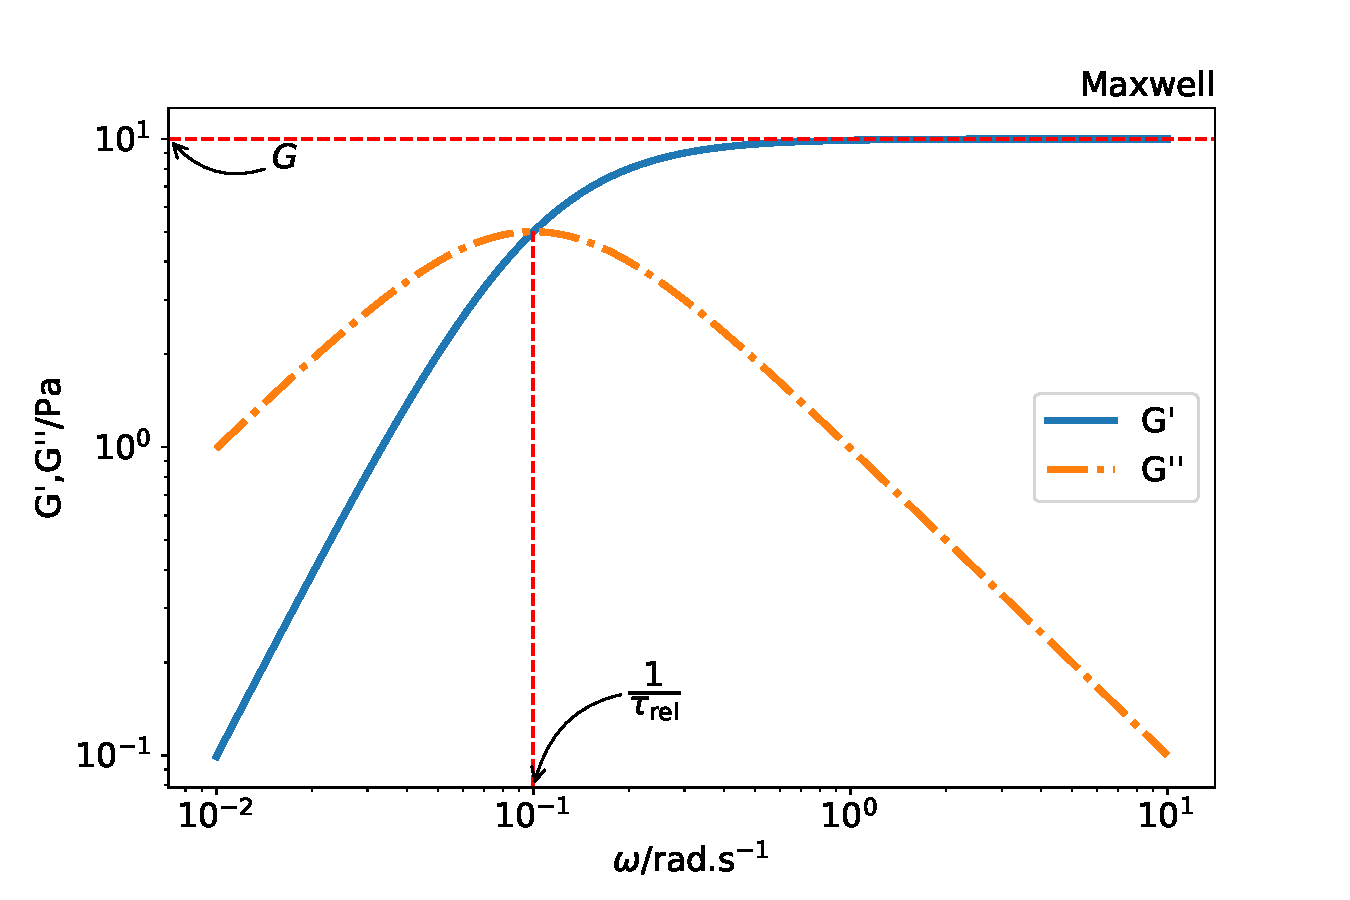
\includegraphics[width=0.7\textwidth]{./imagens/reologia/modelo_maxwell}
				\caption{Espectro mecânico de acordo com o modelo de Maxwell}
				\label{fig:modelo_maxwell}
			\end{figure} \index{reologia!espectro mecânico}
			
			Para o modelo de Maxwell, a viscosidade complexa segue a \autoref{eqn:visc_complexa_maxwell}, sendo que \(\eta_0\) é equivalente à viscosidade no repouso (\autoref{fig:reol_pseudoplastico_loglog}). Não há dependência da tensão \(\gamma\) porque as medidas oscilatórias são obtidas no regime linear.\cite{Rehage1991}
			
			\begin{equation}
				 \eta^* (\omega) = \dfrac{\eta_0}{\left( 1 + \omega^2 \tau_\mathrm{rel}^2 \right)^{\sfrac{1}{2}}}
				\label{eqn:visc_complexa_maxwell}
			\end{equation} \index{reologia!viscosidade complexa \(\eta^*\)}
			
			É possível também relacionar a viscosidade no repouso, \(\eta_0\), obtida nas curvas de fluxo, com os parâmetros \(G\) e \(\tau_{\mathrm{rel}}\), obtidos na reologia oscilatória.\cite{Rehage1991} \index{reologia!relação entre linear e não linear}
			
			\begin{equation}
				\eta_0 = G \tau_{\mathrm{rel}}
				\label{eqn:eta0_g0_taurel}
			\end{equation}  
			
%			Micelas gigantes, em vários regimes, obedecem muito bem o modelo de Maxwell. É possível interpretar esse comportamento da seguinte maneira. Em baixas frequências de perturbação (longos tempos), as micelas possuem tempo suficiente para deslizar umas pelas outras, então a maior parte da energia fornecida é perdida, logo o módulo viscoso, ou de perda, possui valores altos. Em frequências altas, a rede micelar e os entrelaçamentos conseguem armazenar a energia, não possuindo tempo suficiente para deslizar, então o módulo elástico, ou de armazenamento, é alto. Na região intermediária, ambos os mecanismos estão presentes, parte da energia é perdida e parte é armazenada, sendo que no ponto de cruzamento, exatamente metade da energia é preservada e metade é perdida.
			
			Para a obtenção de valores confiáveis para os parâmetros \(G\) e \(\tau_{\mathrm{rel}}\), é necessário realizar um ajuste dessas curvas. Porém, ambos G' e G'' são descritos pelo mesmo conjunto de parâmetros. Ao invés de se fazer dois ajustes e encontrar quatro parâmetros, é ideal realizar um ajuste das duas curvas simultaneamente. Isso pode ser feito pelo software Origin\textregistered, escolhendo uma opção de ajuste de equações, não de expressão. Além disso, é possível utilizar o Excel, com a ferramenta \emph{Solver} para minimizar o conjunto dos resíduos de ambas as curvas. Esse foi o princípio dos ajustes neste trabalho, mas utilizando Python.
			
			\subsection{Modelos mais complexos}
			\label{sec:modelos_complexos_reologia}
			Experimentalmente, existem divergências entre o modelo de Maxwell e os espectros mecânicos dos materiais, especialmente em frequências mais altas, onde modos de movimentação Rouseanos e \emph{breathing modes} podem afetar a reologia.\cite{Berret1993a} Para isso, existem alguns modelos que visam corrigir o modelo de Maxwell, afetando principalmente essa região.\cite{Garcia2018}
			
			Uma possível correção é utilizar dois elementos de Maxwell em série, produzindo um modelo que tem dois tempos de relaxação e dois módulos.\cite{Helgeson2010d} Inclusive, é possível construir um modelo com um número arbitrário de elementos Maxwellianos.\cite{Lyklema_rheology} \index{reologia!Modelos!Dois Modos}
			
			\begin{equation}
				G' = \dfrac{ G_1 \omega^2 \tau_{\textrm{rel,1}}^2   }{  1 + \omega^2 \tau_{\textrm{rel,1}}^2      } + \dfrac{ G_2 \omega^2 \tau_{\textrm{rel,2}}^2   }{  1 + \omega^2 \tau_{\textrm{rel,2}}^2      }
			\label{eqn:modelo_doismodos_g1}
			\end{equation}
		
			\begin{equation}
				G'' = \dfrac{  G_1 \omega  \tau_{\textrm{rel,1}}        }{ 1 + \omega^2 \tau_{\textrm{rel,1}}^2 } + \dfrac{  G_2 \omega  \tau_{\textrm{rel,2}}        }{ 1 + \omega^2 \tau_{\textrm{rel,2}}^2 }
			\label{eqn:modelo_doismodos_g2}
			\end{equation}

			O modelo de Oldroyd é praticamente idêntico ao modelo de Maxwell, e introduz somente um termo relativo à resistência do solvente para altas frequências de G'' (\autoref{eqn:modelo_oldroyd_g2}). G' é inalterado.\cite{Rehage1991, CalabreseTese} Essa é a extensão natural de materiais quase Maxwellianos.\cite{Giant_Micelles}
			\index{reologia!Modelos!Oldroyd}
			
			\begin{equation}
				G'' =\dfrac{  G \omega  \tau_{\textrm{rel}}        }{ 1 + \omega^2 \tau_{\textrm{rel}}^2 } + \eta_{\infty} \times \omega
				\label{eqn:modelo_oldroyd_g2}
			\end{equation}
			
			O modelo mais diferente do modelo de Maxwell é o modelo de Jeffreys, que possui as seguintes formas\cite{Lu2015}: \index{reologia!Modelos!Jeffreys}
			
			\begin{equation}
				G' = \dfrac{G \omega^{2} \tau_{\textrm{rel,1}} \left(\tau_{\textrm{rel,1}} - \tau_{\textrm{rel,2}}\right)}{1 + \omega^{2} \tau_{\textrm{rel,1}}^{2}}
				\label{eqn:modelo_jeffreys_g1}
			\end{equation}
			
			\begin{equation}
				G'' = \dfrac{G \omega \tau_{\textrm{rel,1}} \left(\omega^{2} \tau_{\textrm{rel,1}} \tau_{\textrm{rel,2}} + 1\right)}{1 + \omega^{2} \tau_{\textrm{rel,1}}^{2}}
				\label{eqn:modelo_jeffreys_g2}
			\end{equation}
						
			A \autoref{fig:comparativo_modelos} compara os três modelos mais complexos apresentados com o modelo de Maxwell. \index{reologia!Modelos!comparação dos modelos}
			
			\begin{figure}[h]
				\begin{subfigure}[t]{.5\textwidth}
					\centering
					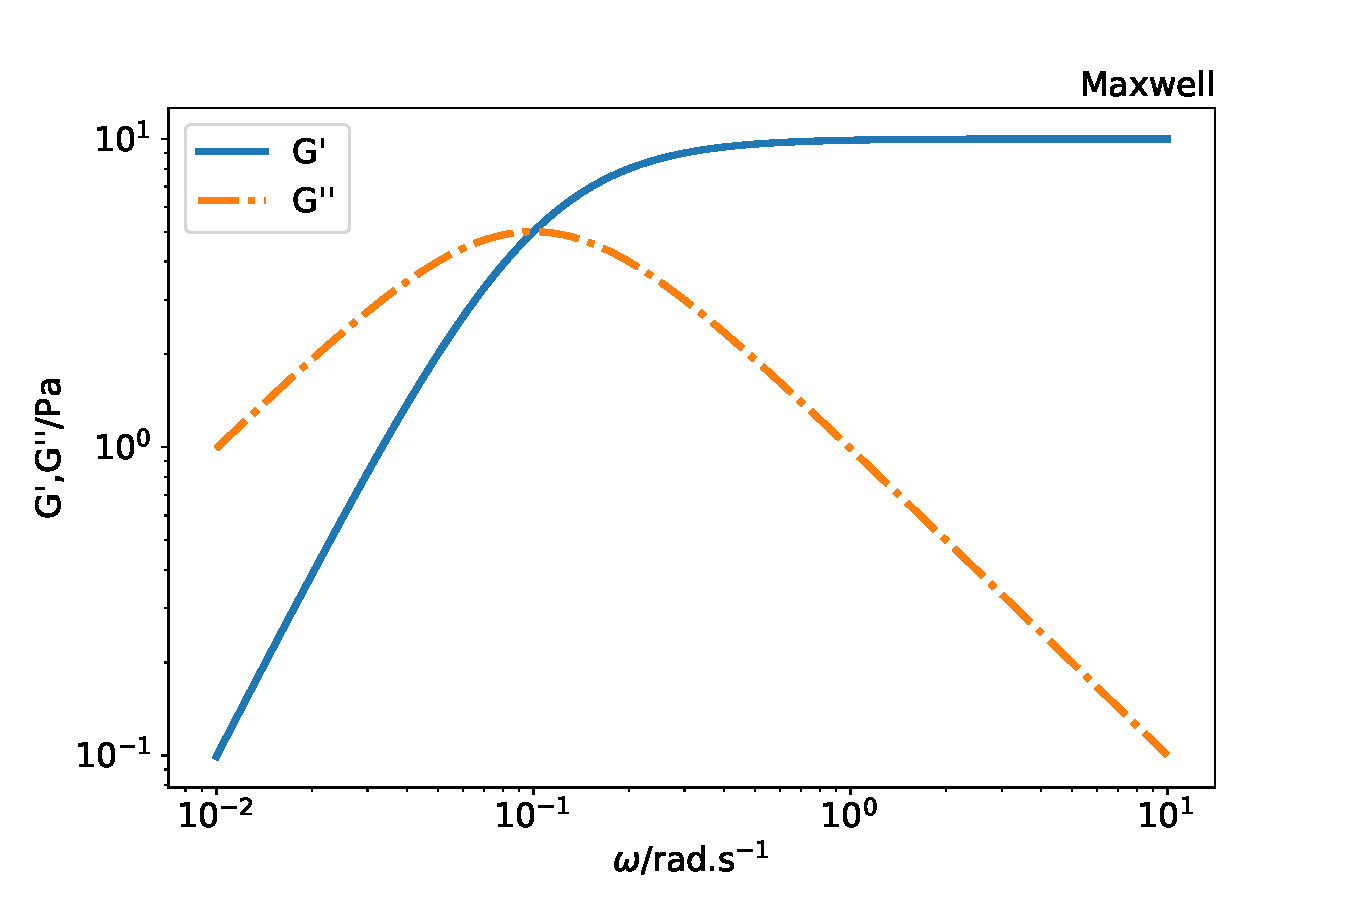
\includegraphics[width=\textwidth]{./imagens/reologia/modelos_comparativo_max}
					\caption{Maxwell. \(G=10, \tau_{\mathrm{rel}}=10\)}
					\label{fig:comparativo_modelo_maxwell}
				\end{subfigure}%
				\begin{subfigure}[t]{.5\textwidth}
					\centering
					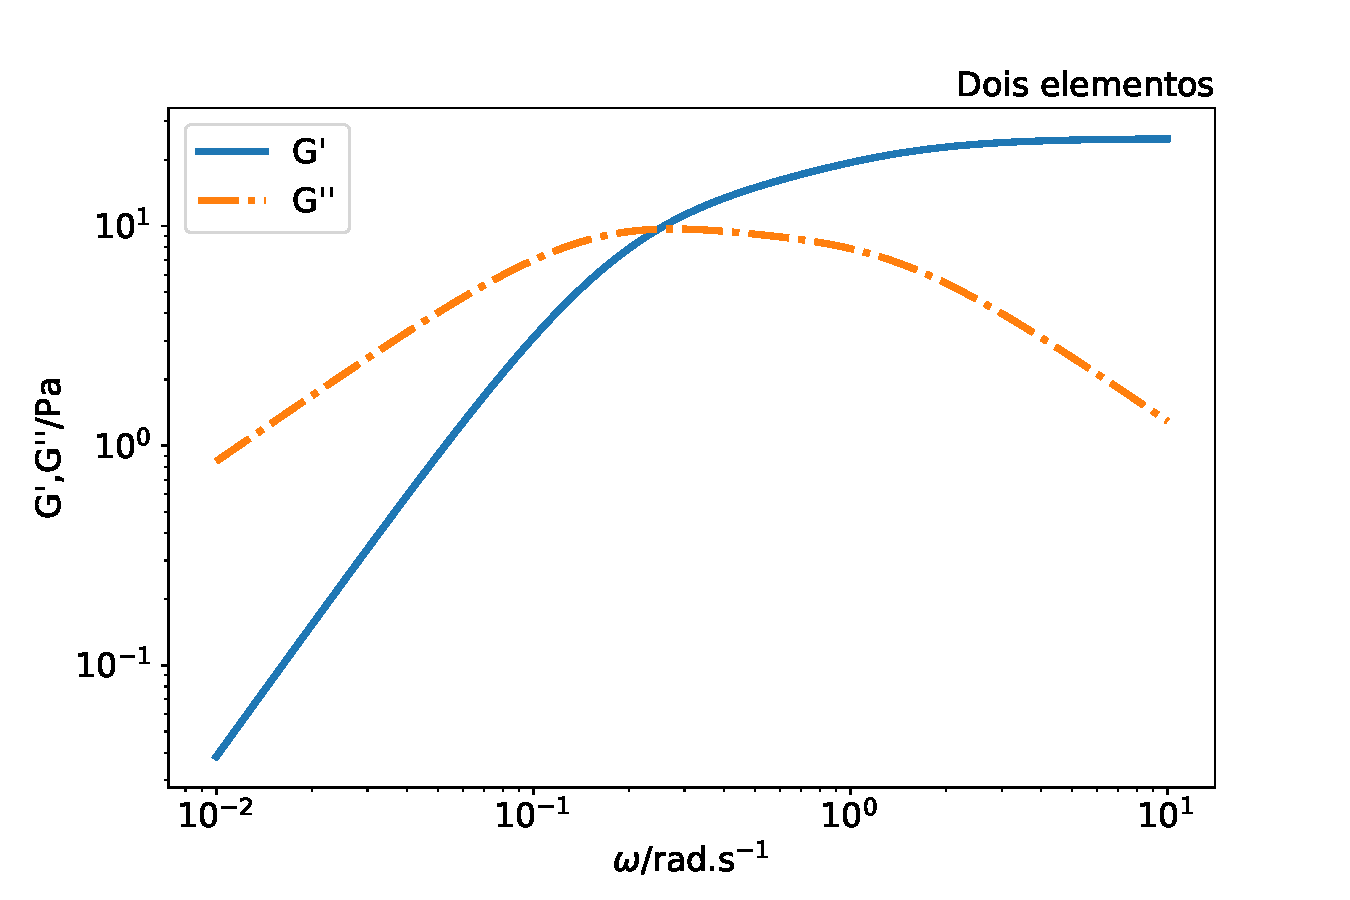
\includegraphics[width=\textwidth]{./imagens/reologia/modelos_comparativo_doismodos}
					\caption{Dois-Modos. \(G_1=10, G_2=15, \tau_{\mathrm{rel,1}}=1,  \tau_{\mathrm{rel,2}}=5\)}
					\label{fig:comparativo_modelo_doismodos}
				\end{subfigure}
			
				\begin{subfigure}[t]{.5\textwidth}
					\centering
					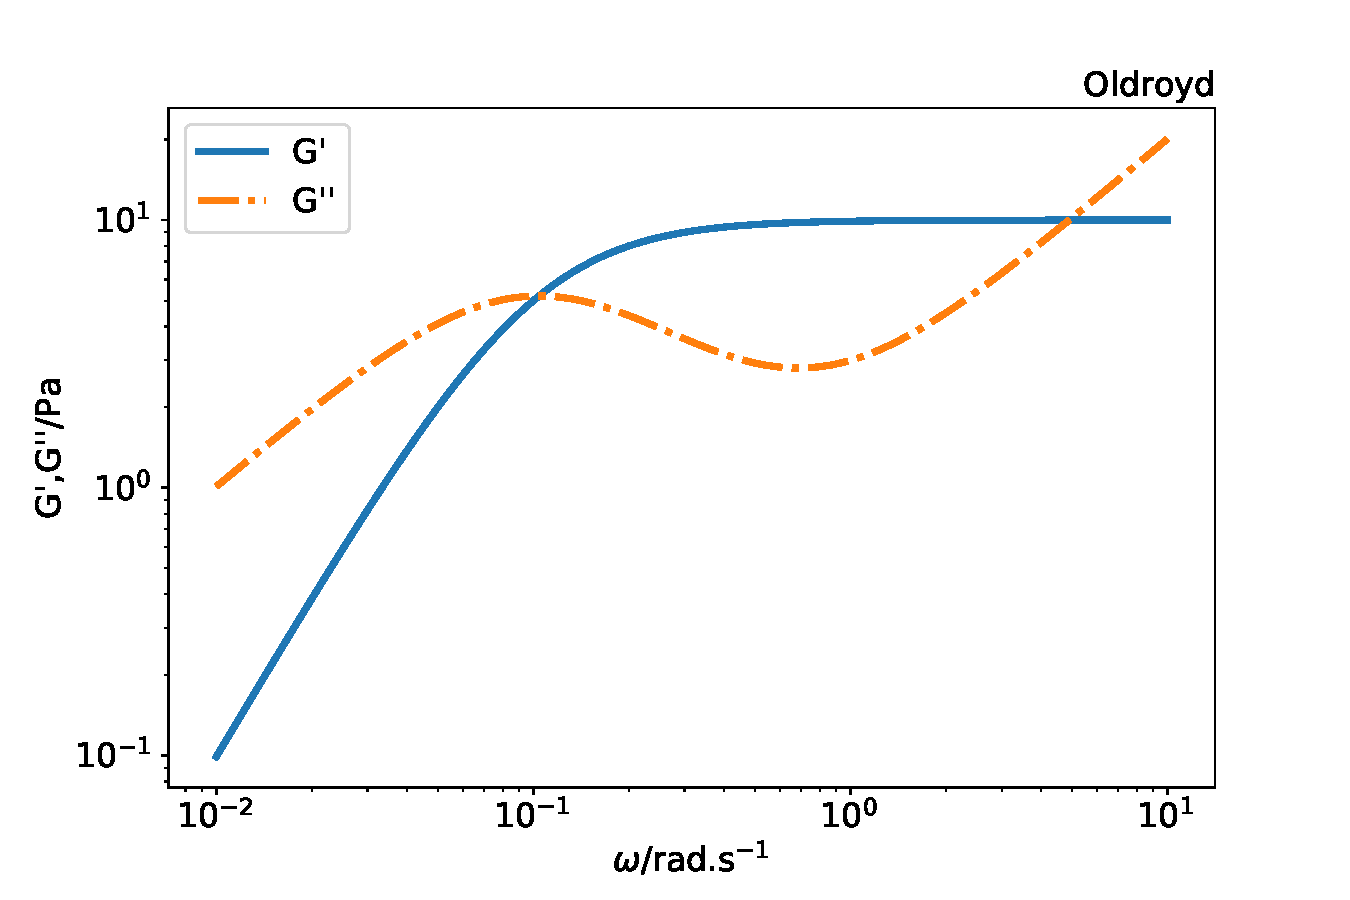
\includegraphics[width=\textwidth]{./imagens/reologia/modelos_comparativo_oldroyd}
					\caption{Oldroyd. \(G=10, \tau_{\mathrm{rel}}=10, \eta_{\infty}=2\)}
					\label{fig:comparativo_modelo_oldroyd}
				\end{subfigure}%	
				\begin{subfigure}[t]{.5\textwidth}
					\centering
					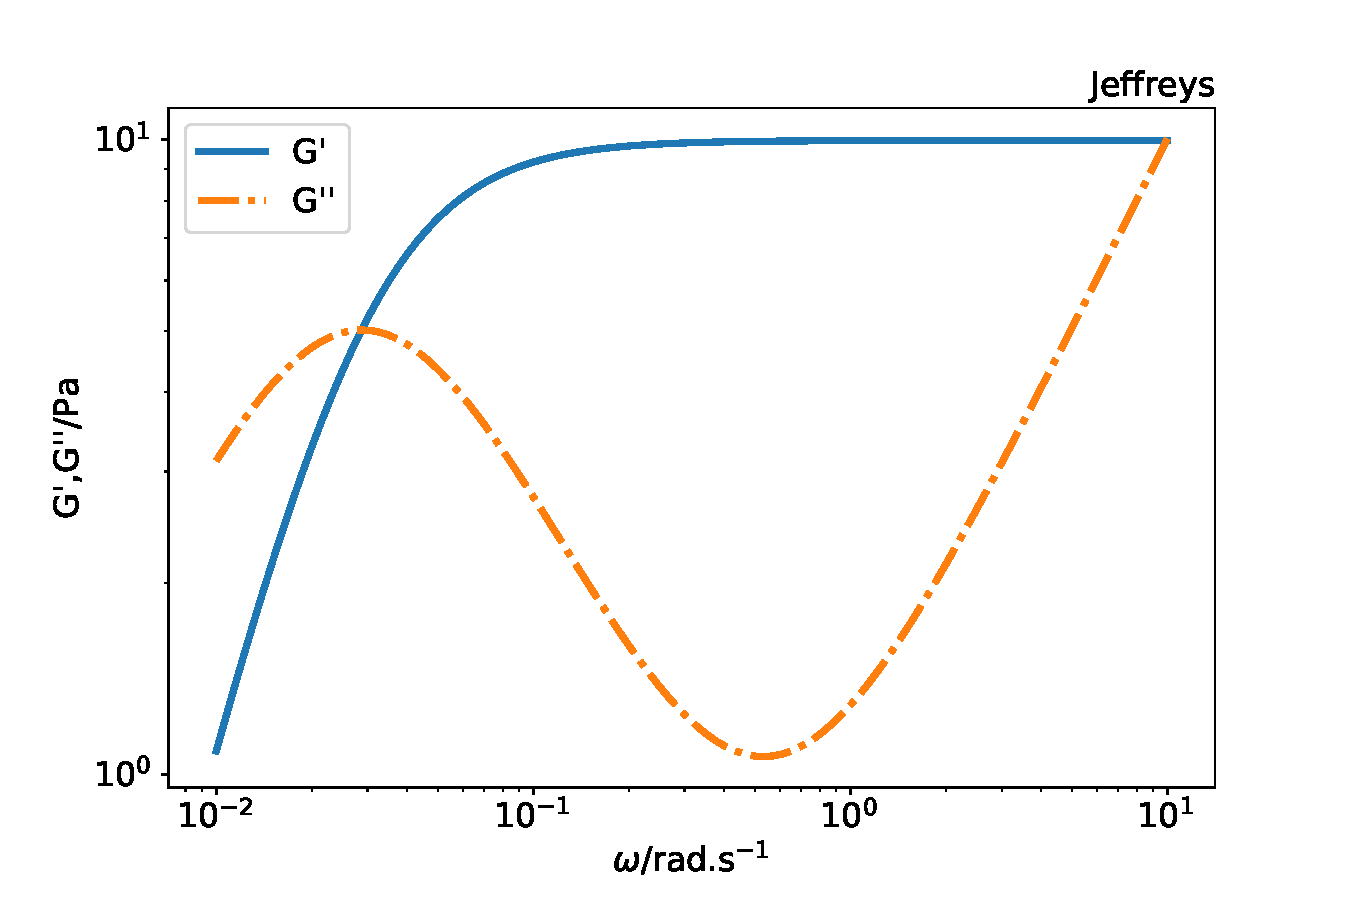
\includegraphics[width=\textwidth]{./imagens/reologia/modelos_comparativo_jeffreys}
					\caption{Jeffreys. \(G=10, \tau_{\mathrm{rel,1}}=35, \tau_{\mathrm{rel,2}}=0.1 \)}
					\label{fig:comparativo_modelo_jeffreys}
				\end{subfigure}
			
				\caption{Comparação dos modelos de Maxwell, Dois-Modos, Oldroyd e Jeffreys. Nas legendas estão os parâmetros para a criação dos modelos. Os módulos estão na unidade de Pa, os tempos de relaxação, em \(s.rad^{-1}\) e \(\eta_{\infty}\) em Pa.s}
				\label{fig:comparativo_modelos}
			\end{figure}
			
			Outro modelo, recentemente proposto por \citeauthor{Garcia2018}, oriundo do modelo de Cates, utiliza um tempo de relaxação para as micelas que é dependente da frequência de oscilação. Nesse modelo, os módulos G' e G'' são praticamente idênticos aos módulos do modelo de Maxwell, porém o tempo de relaxação é composto por um termo \(\tau_{\textrm{rel}, 0}\), que multiplica uma exponencial que possui um termo empírico, \(\beta\). \index{reologia!Modelos!García-Saraji}
			
			\begin{equation}
			G' = \dfrac{ G \omega^2 \tau_{\textrm{rel}}(\omega)^2   }{  1 + \omega^2 \tau_{\textrm{rel}}(\omega)^2  } = %
				 \dfrac{ G \omega^2 \left(  \tau_{\textrm{rel}, 0} e^{-0.5\beta(\omega)}  \right)^2   }{  1 + \omega^2 \left(  \tau_{\textrm{rel}, 0} e^{-0.5\beta(\omega)}  \right)^2  }
			\label{eqn:garcia_saraji_g1}
			\end{equation}
			
			\begin{equation}
			G'' = \dfrac{ G \omega \tau_{\textrm{rel}}(\omega)   }{  1 + \omega^2 \tau_{\textrm{rel}}(\omega)^2  } = %
			      \dfrac{ G \omega \tau_{\textrm{rel}, 0} e^{-0.5\beta(\omega)}   }{  1 + \omega^2 \left(  \tau_{\textrm{rel}, 0} e^{-0.5\beta(\omega)}  \right)^2  }
			\label{eqn:garcia_saraji_g2}
			\end{equation}
			
			\noindent sendo que \(\beta\) é
			
			\begin{equation}
				\beta = a \omega^b
			\end{equation}
			
			\noindent onde \(a\) é o tempo característico da solução viscoelástica, em segundos e \(b\) é a potência da solução viscoelástica, sem dimensão.
			
	\chapter{Calorimetria de titulação isotérmica} \index{ITC} \index{calorimetria de titulação isotérmica|see {ITC}}
	
		\section{Fundamentos} \index{ITC!fundamentos}
		
		% todo: encontrar um termo melhor para ``caixa adiabática''
		
		A calorimetria de titulação isotérmica (ITC) é uma técnica baseada num processo de titulação, onde cada alíquota de titulante resulta em uma ou mais reações químicas ou físicas que podem liberar ou absorver calor. O calor total observado é a somatória do calor de todos esses processos, sendo assim difícil desmembrar as contribuições de cada processo.\cite{Loh2016} No calorímetro há duas celas dentro de uma caixa adiabática; uma de referência, que contém somente água, e outra de amostra, onde ocorre a titulação em si.\cite{Bouchemal2010a} A cela de referência recebe uma quantidade fixa de calor através de uma resistência, e a cela de amostra recebe uma quantidade variável de calor. Isso significa que a temperatura das celas, no decorrer de uma titulação, aumenta ligeiramente, mas menos que 0,1°C. A \autoref{fig:ITC_esquema} ilustra a construção de um calorímetro.
		
		\begin{figure}[h]
			\centering
			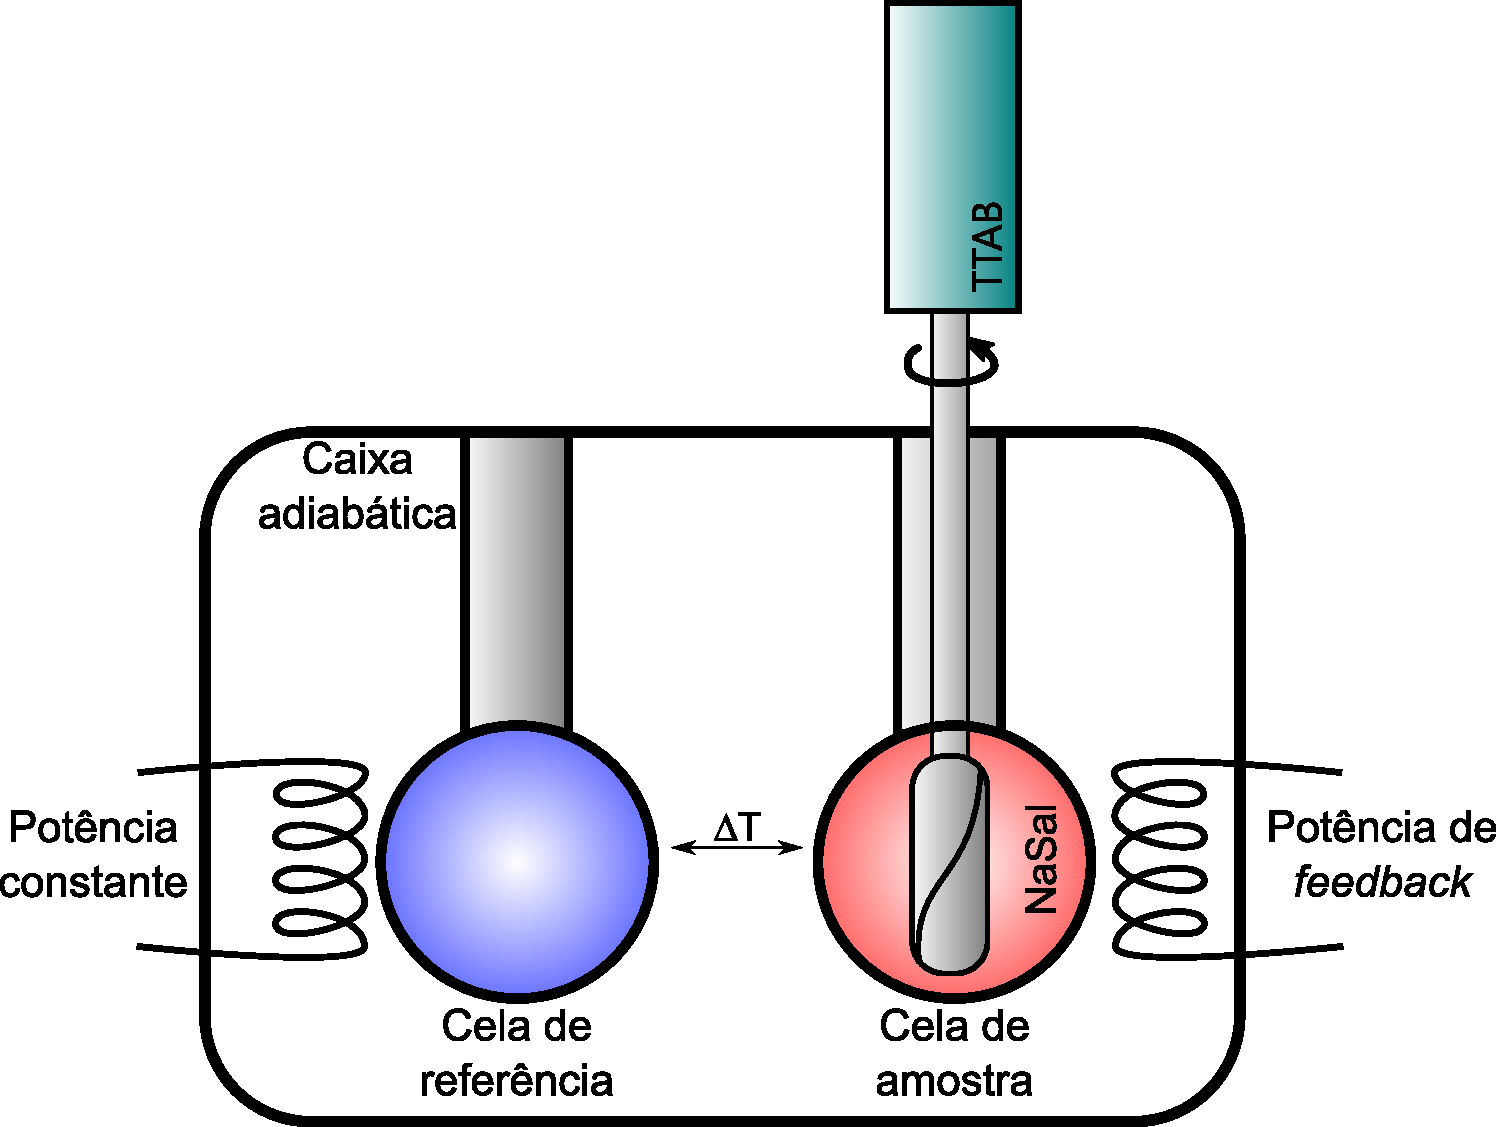
\includegraphics[width=0.5\textwidth]{./imagens/itc/esquema_itc_equipamento}
			\caption{Esquema da construção de um calorímetro de titulação isotérmica}
			\label{fig:ITC_esquema}
		\end{figure} \index{ITC!construção do equipamento}
		
		Durante uma titulação, caso ocorra liberação de calor na cela de amostra, menos energia, em relação ao valor basal, precisa ser fornecida para manter a temperatura igual entre as celas. Caso o sistema absorva calor, mais potência precisa ser fornecida à cela, e vice-versa. Esse comportamento se expressa em picos acima ou abaixo da linha de base. A integração de cada pico no tempo fornece valores de energia que, quando divididos pelo número de mols injetados, obtemos valores de \(\Delta H^0\)/kJ.mol\menosUm. Um diagrama da entalpia pela concentração de titulante é chamada de entalpograma, ou termograma.\cite{Bouchemal2010a}. A \autoref{fig:ITC_exemplo} mostra um exemplo de um experimento de titulação de \TTAB{} em água.
		
		\begin{figure}[h]
			\begin{subfigure}[t]{0.5\textwidth}
				\centering
				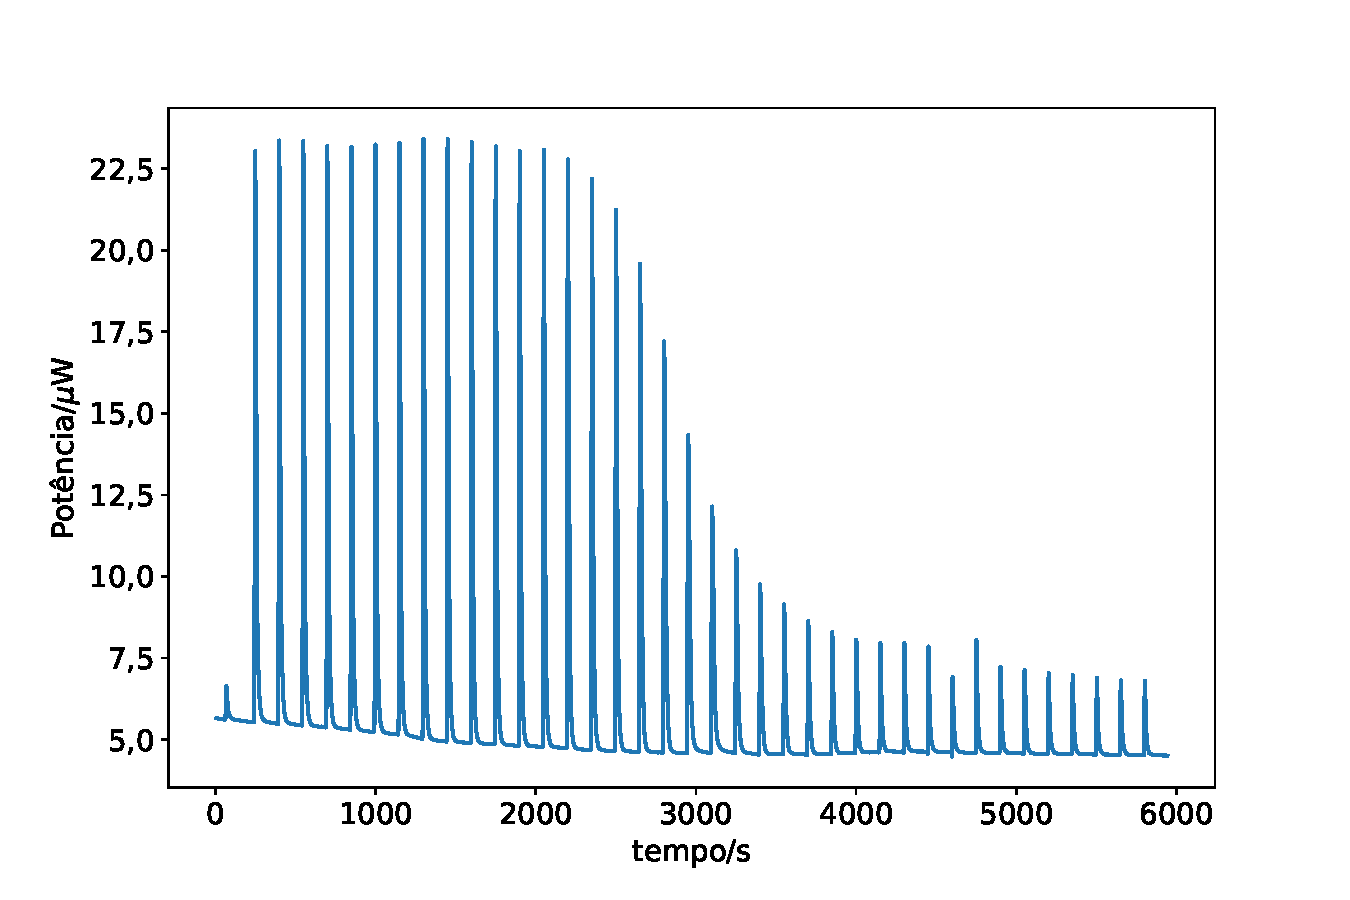
\includegraphics[width=\textwidth]{./imagens/itc/raw_itc_exemplo}
				\caption{Dado bruto}
				\label{fig:ITC_raw_exemplo}
			\end{subfigure}%
			\begin{subfigure}[t]{0.5\textwidth}
				\centering
				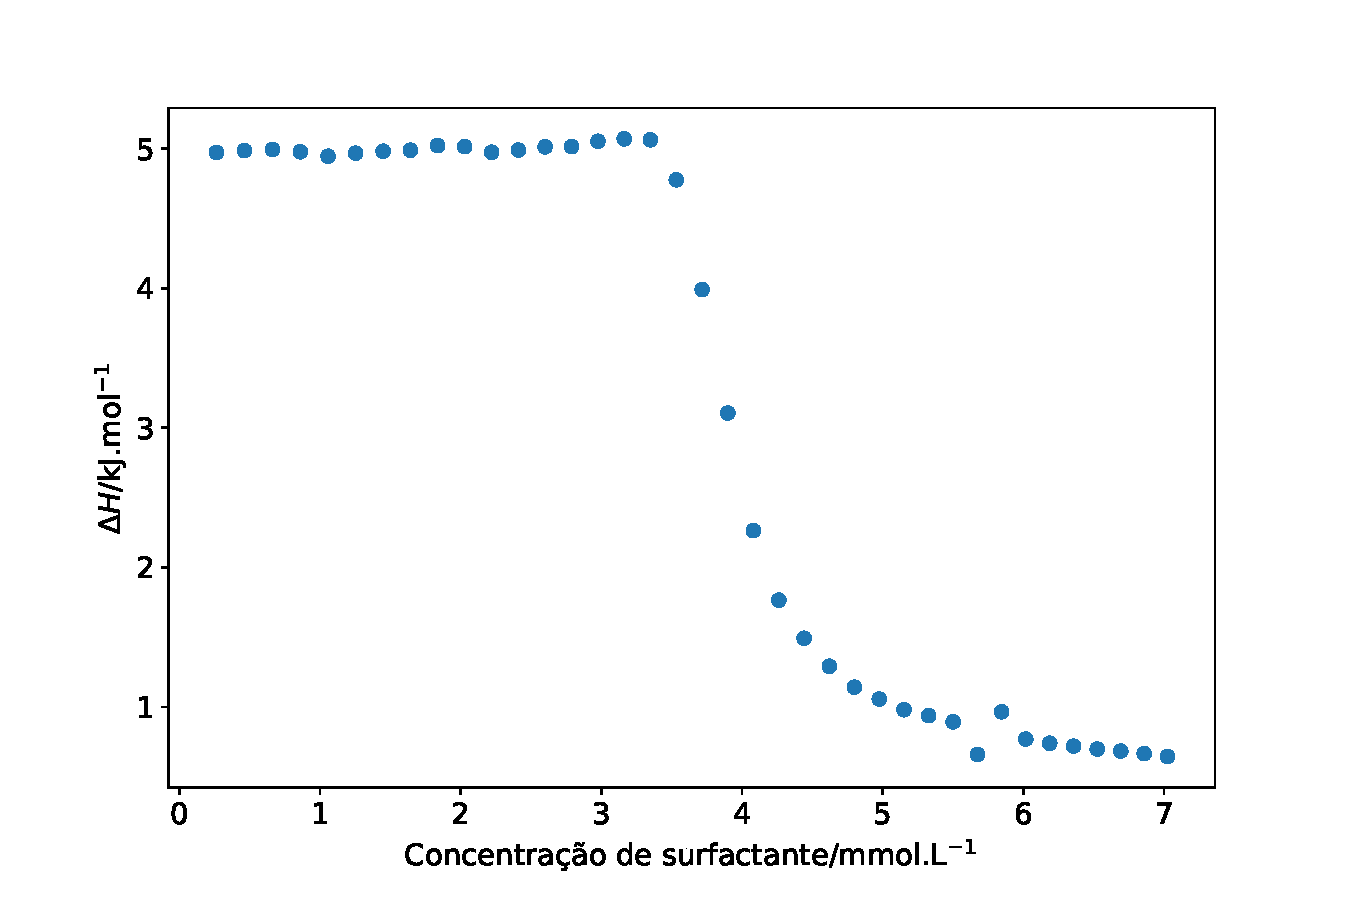
\includegraphics[width=\textwidth]{./imagens/itc/inj_itc_exemplo}
				\caption{Entalpograma}
				\label{fig:ITC_inj_exemplo}
			\end{subfigure}
		
			\caption{Titulação de \TTAB{} 42 \mM{} em água, mostrando o calor absorvido pela célula durante a titulação (\ref{fig:ITC_raw_exemplo}). A primeira injeção é descartada para garantir que as injeções subsequentes possuam um volume correto de injeção. A integração dos picos em relação à linha base, dividindo-se pela concentração de surfactante injetado, resulta no entalpograma (\ref{fig:ITC_inj_exemplo})}
			\label{fig:ITC_exemplo}
		\end{figure}
		
		\FloatBarrier
		
		\section{Calorimetria de micelização} \index{ITC!micelização}
		\label{sec:calorimetria_micelizacao}
		A partir de um conjunto de dados como os da \autoref{fig:ITC_exemplo}, é possível calcular a concentração micelar crítica (\cmc) e a entalpia de micelização, \DHmic. A \cmc{} é dada pelo ponto onde a primeira derivada do entalpograma é máxima (ou mínima)\cite{Bouchemal2010a}, ou onde a segunda derivada é igual a zero.\cite{Sarac2009}  A \DHmic{} é determinada realizando-se dois ajustes lineares das regiões iniciais e finais do entalpograma.\cite{Loh2016} A diferença de entalpia dos pontos de intersecção desses ajustes com uma reta horizontal na \cmc{} fornece o \DHmic{} sem correção.  A \autoref{fig:itc_extracao_cmc_dh} mostra esse método.
		
		\begin{figure}[h] \index{ITC!\cmc}
			\centering
			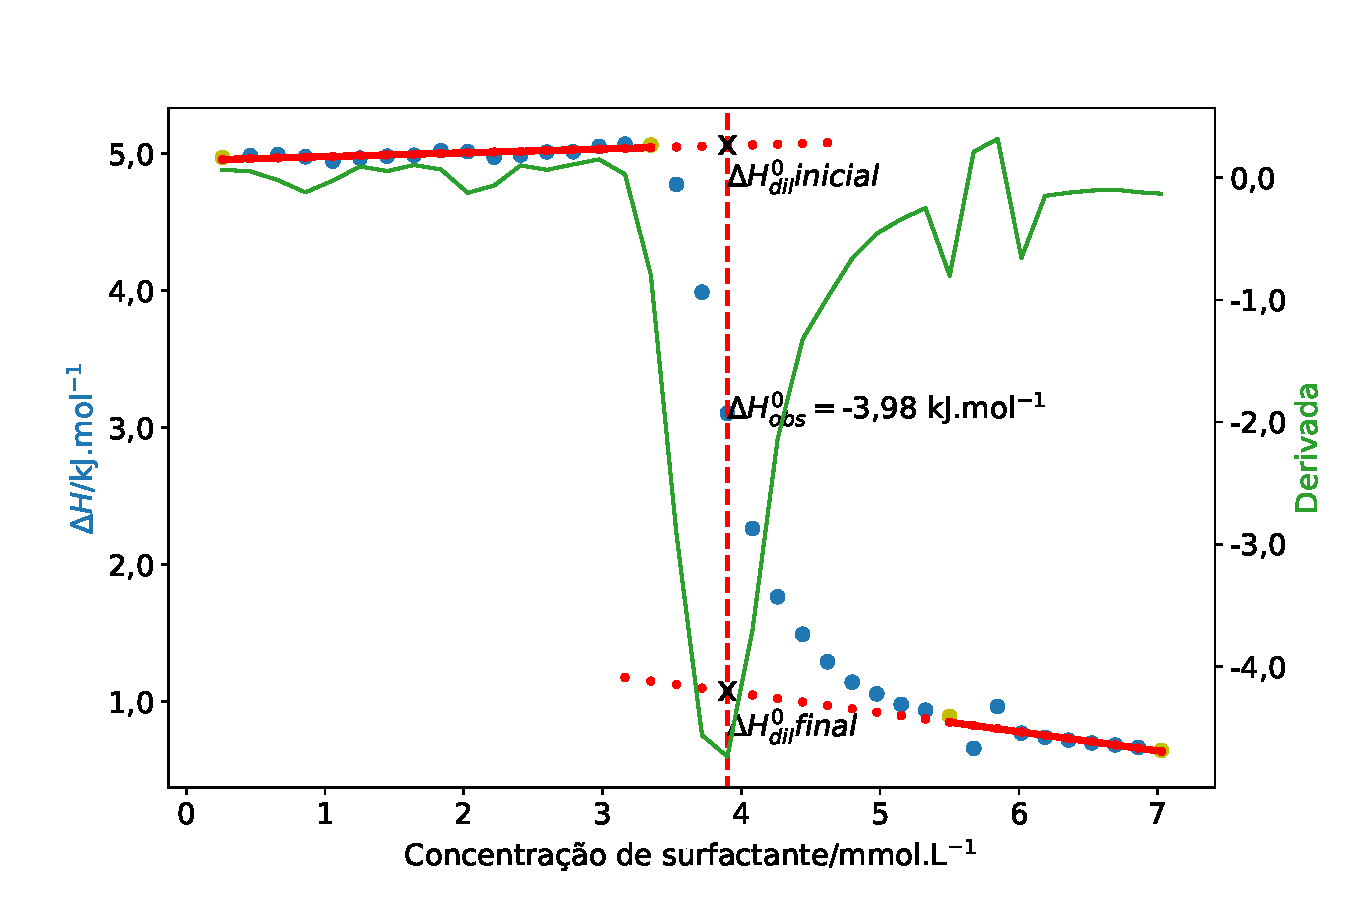
\includegraphics[width=0.7\textwidth]{imagens/itc/extracao_cmc_dh_exemplo}
			\caption{Método para extração da concentração micelar crítica (\cmc) e a entalpia de micelização \DHmic. A curva em verde é a derivada do entalpograma. Os pontos amarelos limitam as regiões onde são feitos ajustes lineares.}
			\label{fig:itc_extracao_cmc_dh}
		\end{figure} 

		Para corrigir a entalpia de micelização observada para obter a entalpia de micelização correta, utiliza-se a \autoref{eqn:itc_obtencao_dhmic}.\cite{Loh2016}  \index{ITC!cálculo de \DHmic}
		
		\begin{equation}
			\Delta H^\circ_{\textrm{mic}} = \Delta H^\circ_{\textrm{obs}} \times \dfrac{c_{\textrm{seringa}}}{c_{\textrm{seringa}-\mathrm{CMC}}}
			\label{eqn:itc_obtencao_dhmic}
		\end{equation}  % todo: ficar de olho aqui porque tem termos que não estão em macros e precisam ser revistos quando algo mudar
		
		\noindent onde \(c_{\mathrm{seringa}}\) é a concentração de surfactante na seringa.
		
		Pela \cmc{} é possível obter a energia livre de micelização a partir da \autoref{eqn:itc_DeltaG_mic}, oriunda do modelo de ação das massas\cite{Loh2016} dependendo do tipo de surfactante e do meio.
		
		\begin{equation}
			\Delta G_{\textrm{mic}}^\circ
			\begin{cases}
			= RT\ln(\chi_{\textrm{cmc}})      & \textrm{Surfactante não iônico}      \\
			= (2-\alpha)RT\ln(\chi_{\textrm{cmc}}) & \textrm{Surfactante iônico}					\\
			\end{cases}
			\label{eqn:itc_DeltaG_mic}
		\end{equation} \index{ITC!relações termodinâmicas}
		
		\noindent onde \(\alpha\) é o grau de ionização das micelas e \(\chi_{\mathrm{cmc}}\) é a concentração micelar crítica em fração molar. O cálculo para surfactantes iônicos assume que o solvente é água e/ou a força iônica seja baixa. Não considerar os contraíons geralmente leva a erros significativos.\cite{Bouchemal2010a}
		
		Com a entalpia e energia livre de micelização, é possível encontrar a entropia de micelização pela equação de Gibbs (\autoref{eqn:itc_gibbs_para_entropia}).
		
		\begin{equation}
			T\Delta S^\circ_{\textrm{mic}} = \Delta H^\circ_{\textrm{mic}} - \Delta G^\circ_{\textrm{mic}}
			\label{eqn:itc_gibbs_para_entropia}
		\end{equation}
		
		Outra maneira de se obter esses parâmetros é pelo ajuste de um modelo, como mostrado em \citeauthor{Sarac2017a}.
		
		Geralmente, em artigos sobre calorimetria, são calculados esses parâmetros termodinâmicos, além da variação de capacidade calorífica \(\Delta C_p\). Com essas informações, se discute a contribuição hidrofóbica\cite{Sarac2017a, Kfouri2019}, o efeito de um sal/aditivo\cite{Sarac2009, Liu2011a, Ito2016}, a espontaneidade de agregação\cite{Ito2016}, e inclusive, cinética de processos.\cite{Kfouri2019,Lof2007a}
		
	\chapter{SAXS} \index{SAXS} \index{espalhamento de raios-X em baixos ângulos |see {SAXS}}
		\section{Fundamentos} \index{SAXS!fundamentos}
		
		%Este capítulo foi fortemente inspirado pelo livro de \citeauthor{Glatter2018livro}, uma excelente, e acessível, introdução à técnica. Os trabalhos de Pedersen também são de boa qualidade, e, quando utilizados, serão indicados.
		
		A radiação eletromagnética é composta com um campo magnético e um campo elétrico oscilantes. Quando um feixe eletromagnético incide sobre uma amostra fina, o campo elétrico variante irá interagir com os elétrons dos átomos dentro da região iluminada. Dependendo da frequência (\(\omega\)), pode ocorrer o fenômeno da absorção perto do limite de Lorentz, \(\omega \approx \omega_0\), de interesse em experimentos espectroscópicos, ou pode ocorrer uma polarização dos átomos que varia com a frequência da radiação quando \(\omega \ll \omega_0\) ou \(\omega \gg \omega_0\). Os dipolos emitem radiação pois toda carga elétrica emite um campo elétrico em direções praticamente aleatórias, com amplitude proporcional à aceleração. Isso é chamado de espalhamento. Essas ondas espalhadas interagem construtiva- e destrutivamente, originando padrões de espalhamento dependendo da localização dos centros espalhadores.\cite{Glatter2018livro}
		
		Raios-X possuem comprimentos de onda tão pequenos que se encontram no limite de Thomson, onde \(\omega \gg \omega_0\). No campo da matéria mole, a energia dos fótons é tão alta que todos os elétrons dos átomos, até suas camadas mais internas, oscilam junto com a radiação. Isso não acontece com o espalhamento de luz, onde a oscilação ocorre somente com os elétrons das camadas mais externas, dependendo da polarizabilidade dos átomos, que é proporcional ao índice de refração do material (\autoref{eqn:lorenz_lorentz}).\cite{Glatter2018livro}
		
		As ondas emitidas, quando comparadas com o feixe incidente, são coerentes, isto é, possuem somente uma diferença de fase \(\varphi\) fixa entre a radiação incidente e espalhada. Além disso, possuem o mesmo comprimento de onda da radiação incidente, então o espalhamento é completamente elástico. Dessa maneira, os vetores incidentes \(\mathbf{k_i}\) e espalhados \(\mathbf{k_s}\) possuem a mesma amplitude, igual ao número de onda \(k\) (\autoref{eqn:numero_onda}), com o índice de refração próximo à unidade, 
		
		\begin{equation} 
			k = \dfrac{2 \pi}{\lambda}
			\label{eqn:numero_onda}
		\end{equation} \index{SAXS!número de onda}
		
		\noindent onde \(\lambda\) é o comprimento de onda da radiação.\cite{Glatter2018livro}
		
		A única diferença entre os feixes espalhados é a fase \(\varphi\) da radiação, devido ao caminho diferente que cada feixe precisa fazer. A diferença de fase de um comprimento de onda é \(2\pi\). Essa fase está relacionada com a interferência dos feixes e, para obtê-la, é necessário subtrair os vetores incidente e espalhado, que passam por um ponto \(P\), cuja posição é dada pelo vetor \(\mathbf{r}\), multiplicados pelo número de onda \(k\),
		
		\begin{equation}
			\varphi = - \left( \dfrac{2\pi}{\lambda} \right) \mathbf{r} \cdot \left( \mathbf{k_s} - \mathbf{k_i} \right)
			\label{eqn:calculo_fase_saxs}
		\end{equation}
		
		O sinal negativo na \autoref{eqn:calculo_fase_saxs} é devido à inversão da ordem de subtração dos vetores \(\mathbf{k_i}\) e \(\mathbf{k_s}\).\cite{Glatter2018livro} Assim, podemos introduzir o vetor de espalhamento \(\mathbf{q}\), também conhecido como vetor de transferência de momento,\cite{Glatter2018livro}
		
		\begin{equation}
			\mathbf{q} = \left( \dfrac{2\pi}{\lambda} \right) \cdot \left( \mathbf{k_s} - \mathbf{k_i} \right)
			\label{eqn:vetor_espalhamento}
		\end{equation} 
		
		Logo, a defasagem pode ser relacionada com a posição dos centros espalhadores e o vetor de espalhamento\cite{Glatter2018livro}
		
		\begin{equation}
			\varphi = - \mathbf{q} \cdot \mathbf{r}
			\label{eqn:defasagem_qr}
		\end{equation}
		
		Uma consequência do produto escalar da \autoref{eqn:defasagem_qr} é que somente a componente de \(\mathbf{r}\) na direção de \(\mathbf{q}\) é relevante para a fase \(\varphi\). Isso implica que todos os pontos num plano perpendicular a \(\mathbf{q}\) possuirão a mesma fase. Isso dá origem à ideia de que o espalhamento ocorre como uma reflexão da radiação por um conjunto de planos, comumente utilizado em cristalografia.\cite{Glatter2018livro}
		
		A amplitude do vetor de espalhamento é dado pela \autoref{eqn:amplitude_vetor_espalhamento}, onde \(\theta\) é o ângulo de espalhamento, entre os vetores \(\mathbf{k_i}\) e \(\mathbf{k_s}\). A \autoref{fig:esquema_saxs} ilustra os vetores incidente e espalhado, assim como o cálculo do vetor.\cite{Glatter2018livro}
		
		\begin{equation}
		q = \dfrac{4\pi}{\lambda} \sin\left(\dfrac{\theta}{2}\right)
		\label{eqn:amplitude_vetor_espalhamento}
		\end{equation} \index{SAXS!vetor de espalhamento \q}
		

		\begin{figure}[h]
			\centering
			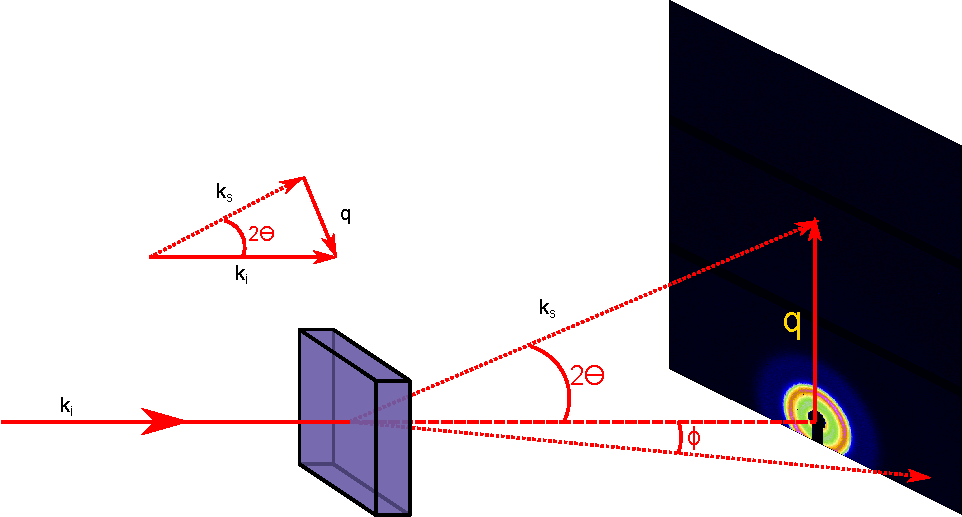
\includegraphics[width=0.7\textwidth]{imagens/saxs/Esquema_SAXS}
			%\caption[Diagrama mostrando o feixe incidente de raios-X sendo espalhado por um material, resultando num vetor espalhado.]{Diagrama mostrando o feixe incidente de raios-X sendo espalhado por um material, resultando num vetor espalhado. O vetor de espalhamento, \(\mathbf{q}\) é paralelo à subtração vetorial dos vetores \( \mathbf{k_i} \) e \( \mathbf{k_s} \), paralelos à direção dos feixes incidente e espalhado. Os feixes, após interagirem, atingem o detector, e a imagem resultante é composta pela contagem de fótons em cada pixel. O ponto escuro é resultante do bloqueio da radiação não espalhada pelo \emph{beam-stop}. Imagem inspirada em \citeauthor{Narayanan2008a}}
			\caption{Diagrama mostrando o feixe incidente de raios-X sendo espalhado por um material, resultando num vetor espalhado. O vetor de espalhamento, \(\mathbf{q}\) é paralelo à subtração vetorial dos vetores \( \mathbf{k_i} \) e \( \mathbf{k_s} \), paralelos à direção dos feixes incidente e espalhado. Os feixes, após interagirem, atingem o detector, e a imagem resultante é composta pela contagem de fótons em cada pixel. O ponto escuro é resultante do bloqueio da radiação não espalhada pelo \emph{beam-stop}. Imagem inspirada em \citeauthor{Narayanan2008a}}
			\label{fig:esquema_saxs}
		\end{figure}
		
		Para pequenos valores de \(\sfrac{\theta}{2}\), \(\sin(\sfrac{\theta}{2}) \approx \sfrac{\theta}{2}\), então a magnitude do vetor de espalhamento \(\mathbf{q}\) (que será chamado de \q{} de agora em diante) é proporcional ao ângulo de espalhamento (em radianos).\cite{Glatter2018livro} A unidade do vetor de espalhamento é tipicamente \(nm^{-1}\), mas outra unidade comum é \AA\menosUm, dependendo do comprimento de onda utilizado. Uma grande utilidade de se utilizar o vetor de onda é que o espalhamento se torna independente da fonte de radiação, pois o comprimento de onda já é levado em consideração. Além disso, o inverso de \q{} informa o tamanho dos objetos que geralmente são observados em SAXS. Faixas comuns são de 0,006 a 6 \(nm^{-1}\), o que resulta em estruturas da faixa de 1\(\mu m\) a 1 \(nm\).\cite{Narayanan2008a}

		Para se determinar o padrão obtido na \autoref{fig:esquema_saxs}, é necessário obter a intensidade de espalhamento em cada ponto. Isso necessita, primeiramente, a soma de todas as ondas espalhadas em cada uma das posições. A função de onda genérica para uma das ondas espalhadas é dada por\cite{Pedersen_Aula1}
		
		\begin{equation}
			\psi(\mathbf{q}) = \exp(-i \mathbf{q} \cdot \mathbf{r})
			\label{eqn:funcao_onda_espalhamento}
		\end{equation}
				
		A somatória das funções de onda, \autoref{eqn:SAXS_somatoria_contribs}, resulta na amplitude de espalhamento. \cite{Pedersen_Aula1} O termo \(b_j\) é o comprimento de espalhamento de cada ponto. Para elétrons, seu comprimento de espalhamento é o raio do elétron, \(r_e = 0.2817 \times 10^{-12}\) cm.
		
		\begin{equation}
			A(\mathbf{q}) = \sum_j b_j \exp(-i \mathbf{q} \cdot \mathbf{r})
			\label{eqn:SAXS_somatoria_contribs}
		\end{equation}
		
		Porém, a resolução de raios-X geralmente não permite a observação dos elétrons individuais, então a somatória dos comprimentos de espalhamento de todos os elétrons no átomo, dividido pelo seu volume, resulta na densidade de comprimento de espalhamento \(\rho\) (\autoref{eqn:SLD}). Esse termo também é conhecido como SLD, do inglês \emph{scattering length density}.\cite{Pedersen_Aula1}
		
		\begin{equation}
			\rho(\mathbf{r}) = \sum_j \dfrac{b_j}{v}
			\label{eqn:SLD}
		\end{equation} \index{SAXS!densidade de comprimento de espalhamento SLD}
		
		Se a densidade for uniforme, podemos encontrar a densidade a partir da fórmula estrutural do material, \cite{Narayanan2008a}
		
		\begin{equation}
			\rho = \dfrac{n_e d_M N_a}{M_w} r_e
			\label{eqn:rho_uniforme}
		\end{equation}
		
		\noindent onde \(n_e\) é o número de elétrons do material, \(d_M\) é sua densidade (água é 1000 kg/m\textsuperscript{3}), \(N_a\) é o número de Avogadro, \(M_w\) é a massa molar do material e \(r_e\) é o raio do elétron.
		
		Assim, a \autoref{eqn:SAXS_somatoria_contribs} passa de uma somatória para uma integral, \autoref{eqn:SAXS_integral_amplitude}, \cite{Narayanan2008a}
		
		\begin{equation}
			A(\mathbf{q}) = \int_V \rho(\mathbf{r}) \exp(-i \mathbf{q} \cdot \mathbf{r}) d\mathbf{r}
			\label{eqn:SAXS_integral_amplitude}
		\end{equation}
		
		A intensidade de espalhamento, detectada pelo equipamento, é obtida pela média pelo tempo de todas as posições e conformações possíveis das partículas, ao quadrado (multiplicando-se pelo complexo conjugado).\cite{Pecora2008a} É necessário utilizar constantes para normalizar essa intensidade, como o número \(n\) de partículas espalhadoras e o volume \(V\) das partículas. Além disso, como as partículas estão num meio, como um solvente, é necessário considerar a densidade eletrônica do solvente, e por isso utiliza-se \(\Delta \rho^2\), a diferença entre a densidade do solvente e do meio, também conhecido como contraste. Todas essas considerações resultam em\cite{Pedersen_Aula1}
		
		\begin{equation}
		I(q) = n\Delta \rho^2 V^2 |A(q)|^2
		\label{eqn:SAXS_I_funcao_A}
		\end{equation}

		Mais informações sobre o cálculo de figuras de espalhamento podem ser encontrados em \citeauthor{Alves2017}.
		
		Sistemas com alto contraste, por exemplo, partículas de ouro em água, espalham bastante raios-X, resultando em sinais de boa qualidade. Porém sistemas de baixo contraste, como a maior parte de sistemas de materia mole, incluindo o sistema \CTAB{} + NaSal, utilizado neste trabalho, não resultam em uma boa resolução sinal/ruído. Tipicamente, o contraste das cabeças é positivo em relação à água, mas o contraste das cadeias é negativo, o que resulta num contraste total baixo. Logo, é interessante calcular o contraste, o que pode ser feito por programas como o SASfit.\footnote{\url{https://github.com/SASfit/SASfit}}. Algumas vezes é possível melhorar o contraste adicionando-se sacarose ou glicerina ao solvente ao meio, porém isso só é válido para experimentos de SAXS, não de espalhamento de luz, onde a igualdade do índice de refração efetivamente faria os agregados serem invisíveis.
		
		\section{Modelagem e o problema inverso do espalhamento}
		
		O objetivo de análises de SAXS é obter informações estruturais das partículas presentes no meio. Esse é chamado o problema inverso do espalhamento, em contraste com o problema direto, onde estruturas são propostas e o padrão de espalhamento das mesmas é calculado. Para resolver o problema inverso, é necessário primeiramente obter os modelos necessários, um processo matematicamente bastante complexo, e depois ajustá-los às curvas obtidas, variando-se os parâmetros de ajuste pelo método dos mínimos quadrados.\cite{Glatter2018livro} A etapa de ajuste também possui seu grau de dificuldade, necessitando frequentemente de técnicas complementares para a escolha de um modelo e para fornecer chutes iniciais para os parâmetros. 
		
		\subsection{Partículas esféricas homogêneas em solução} \index{SAXS!modelagem!esferas}
		
		Quando se considera o espalhamento de um único objeto não centro-simétrico, é necessário considerar a orientação do vetor de espalhamento \q{} para obter o padrão de espalhamento. Além disso, em solução, esses objetos estão possivelmente orientados aleatoriamente, sendo necessário realizar uma integração sobre todas as orientações possíveis. Porém, objetos centro-simétricos, como esferas de raio \(R\), não necessitam disso.  A amplitude de espalhamento de uma esfera pode ser calculada por \cite{Narayanan2008a, Pedersen_Aula1}
		
		\begin{equation}
			A(q) = \dfrac{4\pi\Delta\rho}{q} \int_0^R \dfrac{\sin(qr)}{r} rdr
			\label{eqn:SAXS_amplitude_esfera}
		\end{equation}
				
		Realizando uma integração parcial, obtemos\cite{Pedersen_Aula1}
		
		\begin{equation}
			A(q) = \Delta\rho \dfrac{4\pi R^3}{3} \left[ \dfrac{3 \left( \sin (qR) - (qR) \cos (qR) \right)}{\left(qR\right)^3} \right]
			\label{eqn:SAXS_amplitude_esfera_integrado}
		\end{equation}
		
		Essa equação, normalizada, será utilizada na descrição do modelo de micelas gigantes (\autoref{eqn:AP_Fsphere}) que está presente no \autoref{sec:modelo_MG_matematica}.
		
		Como a intensidade de luz espalhada é o quadrado da amplitude, \cite{Narayanan2008a}
		
		\begin{equation}
			I(q) = |A(q)|^2 = (\Delta \rho)^2 V_\mathrm{esfera}^2 P=(\Delta \rho)^2 V^2 \left[ \dfrac{3 \left( \sin (qR) - (qR) \cos (qR) \right)}{\left( qR \right) ^3} \right]^2
			\label{eqn:SAXS_intensidade_esfera}
		\end{equation}
		
		% Hiris: Esse fator forma possui?
		O termo à direita da \autoref{eqn:SAXS_intensidade_esfera} é chamado de fator forma \(P\). \index{SAXS!fator forma} Esse fator forma possui vários mínimos em valores de \(qR\) em 4,493, 7,725, etc, como mostra a \autoref{fig:espalhamento_esfera}. Gerar essa figura é fácil, como mostra a listagem \ref{lst:plot_micela_esferica}. A partir desses mínimos é possível obter o raio da partícula, apesar de que isso só é válido para partículas monodispersas, totalmente esféricas, homogêneas e em uma solução diluída. \cite{Pedersen_Aula1, Narayanan2008a}
		
		\begin{figure}[h]
			\centering
			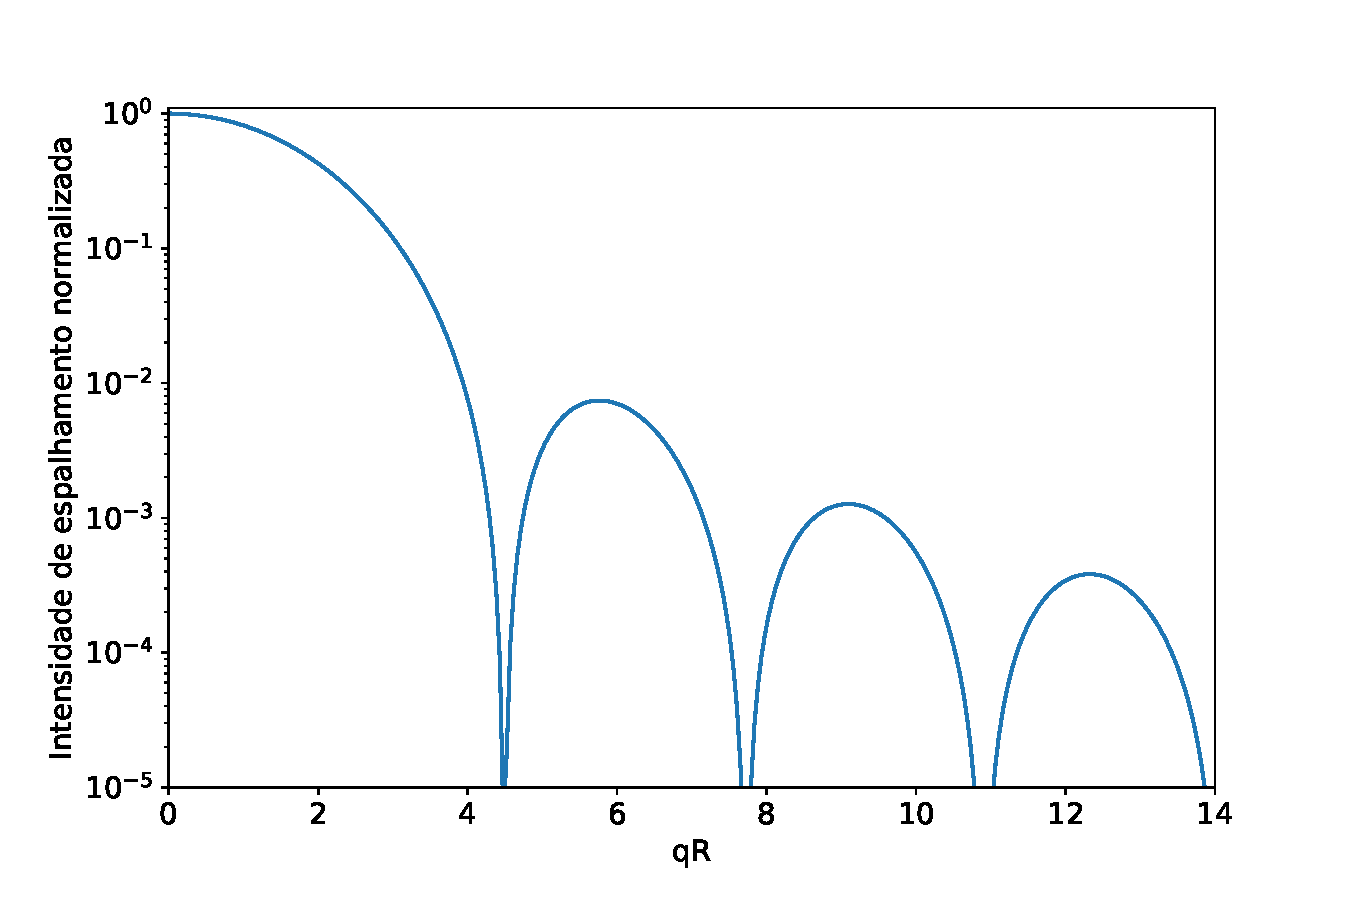
\includegraphics[width=0.7\textwidth]{imagens/saxs/espalhamento_esfera_monodispersa}
			\caption{Espalhamento de uma esfera monodispersa. Os mínimos estão relacionados com o raio da esfera. O código para fazer este gráfico se encontra na listagem \ref{lst:plot_micela_esferica}.}
			\label{fig:espalhamento_esfera}
		\end{figure}
		
		\begin{listing}[h]
			\inputminted{python}{./python/plot_saxs_esfera.py}
			\caption{Código utilizado para a criação da \autoref{fig:espalhamento_esfera}}
			\label{lst:plot_micela_esferica}
		\end{listing}
		
		Esse é o exemplo mais simples para a derivação da amplitude de espalhamento de um objeto. Quanto maior for a complexidade dos objetos modelados, e mais concentrada for a solução, mais difícil fica a derivação dos modelos, exigindo considerável experiência e conhecimento matemático. \citeauthor{Pedersen1997b} mostra uma lista de modelos para vários formatos de partículas. Durante a execução deste trabalho, o Prof. Jan Skov Pedersen, da Universidade de \AA rhus, Dinamarca, adaptou modelos descritos na literatura para descrever sistemas alongados em solução, como polímeros e micelas gigantes. Uma descrição matemática superficial do modelo desenvolvido se encontra no \autoref{sec:modelo_MG_matematica}, e uma adaptação desse modelo na linguagem Python se encontra no \autoref{sec:modelo_MG_python}.
		
		\subsection{Fator estrutura, concentrações altas} \index{SAXS!fator estrutura}
		
		Quando a translação e orientação de uma partícula em solução começa a depender das outras, uma contribuição do espalhamento dessas correlações começa a se tornar visível. Esse fator adicional, chamado de fator estrutura, \(S(q)\), deve ser multiplicado ao \(P(q)\) para se obter o valor da intensidade correta (\autoref{eqn:SAXS_I_P_S}). Em soluções diluídas, a contribuição do fator estrutura se cancela devido à posição e à orientação arbitrárias das partículas, então \(S(q) \approx 1\).\cite{Narayanan2008a}
		
		\begin{equation}
			I(q) = n\Delta \rho^2 V^2 P(q) S(q)
			\label{eqn:SAXS_I_P_S}
		\end{equation}
		
		Como as distâncias entre partículas são tipicamente maiores do que as distâncias dentro das partículas, as contribuições do fator estrutura geralmente aparecem com maior intensidade em valores de \q{} baixos.\cite{Glatter2018livro}
		
		Existem vários modelos possíveis para o fator \(S(q)\), que dependem de uma função que descreve a probabilidade de se encontrar uma partícula a uma distância \(r\) de outra. Dentro dessa função, existe um potencial que pode descrever, por exemplo, se há atração ou repulsão eletrostática entre as partículas. Por exemplo, o modelo das esferas rígidas sem carga, o mais simples, que possui o seguinte potencial \cite{Glatter2018livro}
		
		\begin{equation}
			u(r) = 
			\begin{cases}
				\infty  & r < (R_a + R_b) \\
				0		& r > (R_a + R_b)
			\end{cases}
			\label{eqn:potencial_esfera_rígida}
		\end{equation}

		\noindent onde \(R_a\) e \(R_b\) são os raios de duas partículas que estão interagindo.
		
		A presença de fatores estrutura adicionam alguns parâmetros fortemente não lineares ao ajuste e aumentam grandemente a complexidade dos mesmos, tornando a determinação do fator forma e estrutura simultaneamente uma tarefa bastante difícil. Além disso, quando há polidispersidade nos sistemas, não se torna possível a completa separação dos termos \(P(q)\) e \(S(q)\) (como é o caso das micelas gigantes do \autoref{sec:modelo_MG_matematica}) e é necessário utilizar um fator estrutura efetivo, \(S_m(q)\).\cite{Narayanan2008a}
		
		\subsection{Indexação de picos} \index{SAXS!indexação de picos}
		\label{sec:teoria_SAXS}
		
		Outro exemplo de estruturação é o que ocorre quando existem cristais líquidos em solução. Neste trabalho, observou-se fases lamelares, então receberão o foco do texto. Geralmente, os picos oriundos do fator estrutura se superpõem ao fator forma, tornando-se bastante evidentes. Esses picos são consequência da ordenação equidistante das bicamadas, e a posição dos picos está relacionada à distância média das lamelas.\cite{Glatter2018livro} Outras mesofases também resultam em fatores estrutura, mas com a posição relativa dos picos em valores diferentes, o que permite a identificação da fase a partir de SAXS.\cite{Narayanan2008a} A \autoref{fig:exemplo_saxs} mostra o padrão de espalhamento de uma amostra lamelar, obtido neste trabalho. Essa figura é resultado da integração azimutal da imagem da \autoref{fig:esquema_saxs}.
		
		\begin{figure}[h]
			\centering
			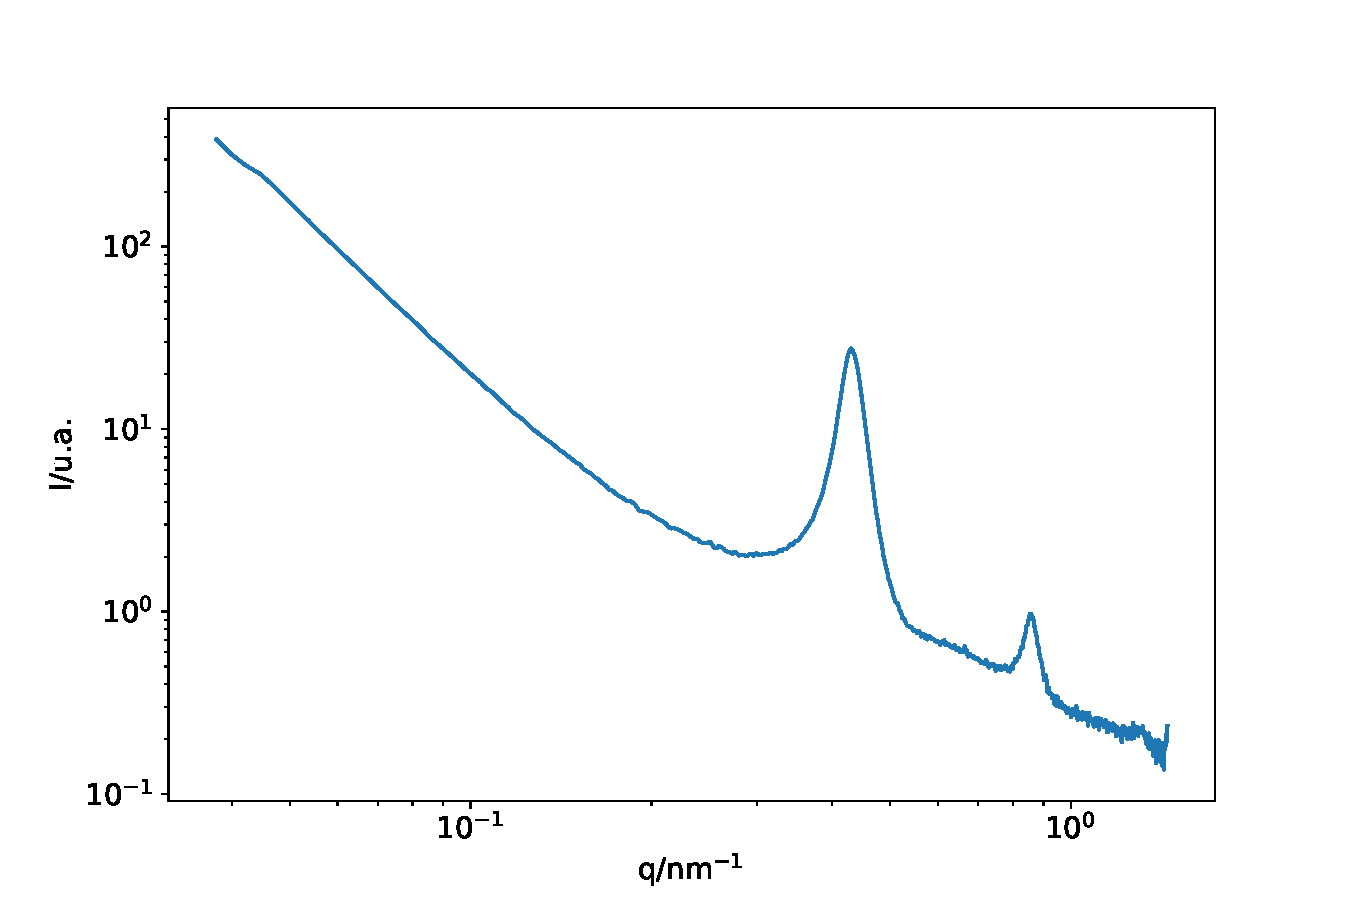
\includegraphics[width=0.7\textwidth]{imagens/saxs/exemplo_SAXS}
			\caption{Curva de espalhamento resultante da integração em \(\phi\) do padrão de espalhamento obtido na \autoref{fig:esquema_saxs}. Os picos obtidos nessa figura são resultado da difração de raios-X devido à presença de uma estrutura lamelar em solução.}
			\label{fig:exemplo_saxs}
		\end{figure}
		
		Com o valor de \q{} do primeiro pico, é possível determinar o parâmetro de rede (\emph{lattice parameter}) da mesofase.\cite{Percebom2018} Para estruturas lamelares, que são de maior relevância para este trabalho, temos que o espaçamento dos picos é de \(1:2:3:4\dots\)\cite{Narayanan2008a} O parâmetro de rede, \(d\), \index{SAXS!parâmetro de rede} é dado pela \autoref{eqn:SAXS_param_rede_lamela}, e seu significado está ilustrado na \autoref{fig:saxs_distancia_interlamelar}. É interessante notar a semelhança desse método de identificação com a determinação do raio de esferas pelos mínimos da \autoref{fig:espalhamento_esfera}. Os picos observados também são chamados de picos de Bragg, mostrando a íntima relação com a área de difração de raios-X, e a modelagem desse tipo de curva de espalhamento utiliza os índices de Miller dos objetos.\cite{Narayanan2008a}
	
		\begin{equation}
			q = \dfrac{2\pi}{d}
			\label{eqn:SAXS_param_rede_lamela}
		\end{equation} 
		
		\begin{figure}[h]
			\centering
			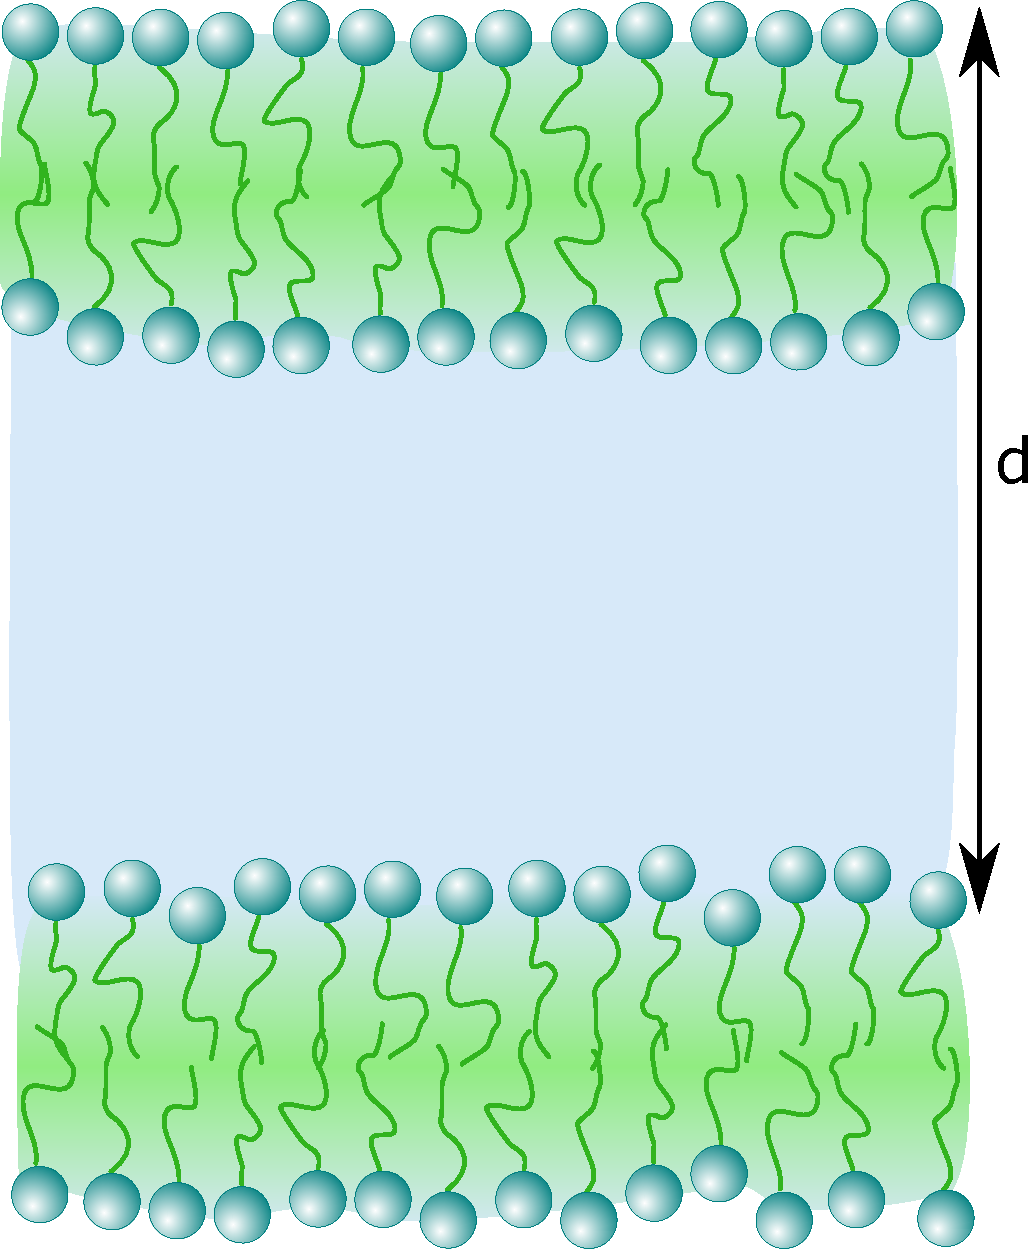
\includegraphics[width=0.35\textwidth]{imagens/saxs/distancia_interlamelar}
			\caption{Distância interlamelar}
			\label{fig:saxs_distancia_interlamelar}
		\end{figure}

		A partir da distância interlamelar, é possível calcular a espessura lamelar (\(d_{\text{HC}}\)) caso a fração volumétrica de surfactante (\(\phi_s\)) e solvente (\(\phi_w\)) também sejam conhecidos. Nesse caso, seria necessário somente relacionar as proporções das regiões com o total, a distância interlamelar. Esse é o princípio do método descrito em \citeauthor{Ferreira2016}. A fração volumétrica de surfactante pode ser obtida pela \autoref{eqn:SAXS_frac_volum}, cujos parâmetros estão explicados na \autoref{tab:ur_fracvol_descr}. \index{SAXS!fração volumétrica de surfactante}
		
		\begin{equation}
			\phi_s = \dfrac{V_{\textrm{HC}}\left( \dfrac{w_{s}}{M_{s}} \right)}{\left( V_{\textrm{HC}} + V_{P} \right)\dfrac{w_{s}}{M_{s}} + V_{w}\dfrac{w_{w}}{M_{w}}}
			\label{eqn:SAXS_frac_volum}
		\end{equation}
		
		\begin{table}[h]
			\IBGEtab{\caption{Descrições das variáveis da \autoref{eqn:SAXS_frac_volum} \label{tab:ur_fracvol_descr}}}
			{\begin{tabular}{r l}
				\toprule
				           Variável & Descrição                                               \\ \midrule
				         \(\phi_s\) & Fração volumétrica de surfactante                       \\
				\(V_{\mathrm{HC}}\) & Volume molar parcial da cadeia alquílica do surfactante \\
				          \(V_{P}\) & Volume molar parcial da cabeça do surfactante           \\
				          \(w_{s}\) & Fração mássica de surfactante                           \\
				          \(M_{s}\) & Massa molar do surfactante                              \\ \midrule
				          \(V_{w}\) & Volume molar parcial de água                            \\
				          \(w_{w}\) & Fração mássica de água                                  \\
				          \(M_{w}\) & Massa molar da água                                     \\ \bottomrule
			\end{tabular}
			}%
			{}%
		\end{table}

		Sabendo então a fração volumétrica de surfactante, podemos obter a espessura da lamela a partir da distância total pela simples relação \cite{Ferreira2016}
		
		\begin{equation} \label{eqn:SAXS_espessura_lamelar} 
			d_{\text{HC}} = \phi_s d
		\end{equation} \index{SAXS!espessura lamelar}
		
		Em suma, o espalhamento de raios-X em baixos ângulos é uma técnica que permite a obtenção de parâmetros estruturais médios microscópicos do sistema, desde que se conheça quais são as estruturas mais prováveis presentes na amostra. Isso é feito através do ajuste de modelos desenvolvidos pela descrição matemática das estruturas, pelo método dos mínimos quadrados, ou também pela indexação de picos.
		
	\chapter{Fluorescência} \index{Fluorescência}
		\section{Diagrama de Jablonski} \index{Fluorescência!Diagrama de Jablonski}
		
		O fenômeno de fluorescência é uma subdivisão do fenômeno luminescência, posição que compartilha com a fosforescência. A diferença entre os dois fenômenos está no mecanismo de transição eletrônica, que também altera os tempos de vida dos dois fenômenos. De forma geral, os tempos de vida de fluorescência são da ordem de \(10^{-8} s\), já a fosforescência os tempos de vida variam de milissegundos a segundos.\cite{Lakowicz2006} Neste trabalho, somente o fenômeno da fluorescência é de importância.
		
		Uma maneira de se visualizar os fenômenos de luminescência é através do diagrama de Jablonski. Nesse tipo de diagrama, o eixo y representa energia, e as várias linhas representam níveis energéticos.\cite{Lakowicz2006} A \autoref{fig:diagrama_jablonski} mostra um diagrama de Jablonski onde os fenômenos de absorção, fluorescência e fosforescência estão ilustrados. Os níveis \(S\) representam os estados singleto, e seu subíndice representa o nível eletrônico, sendo 0 o fundamental. Os níveis vibracionais são marcados de 0 a 4 nesse diagrama, com o estado fundamental marcado com uma linha mais grossa e os outros, com uma linha mais fina. As linhas pontilhadas representam processos não-radiativos e as linhas cheias representam processos radiativos. \index{Fluorescência!processo radiativo} \index{Fluorescência!processo não-radiativo} As cores das linhas são proporcionais aos comprimentos de onda envolvidos, mas não descrevem as cores reais. O nível tripleto é representado como \(T_1\). 
		
		\begin{figure}[h]
			\centering
			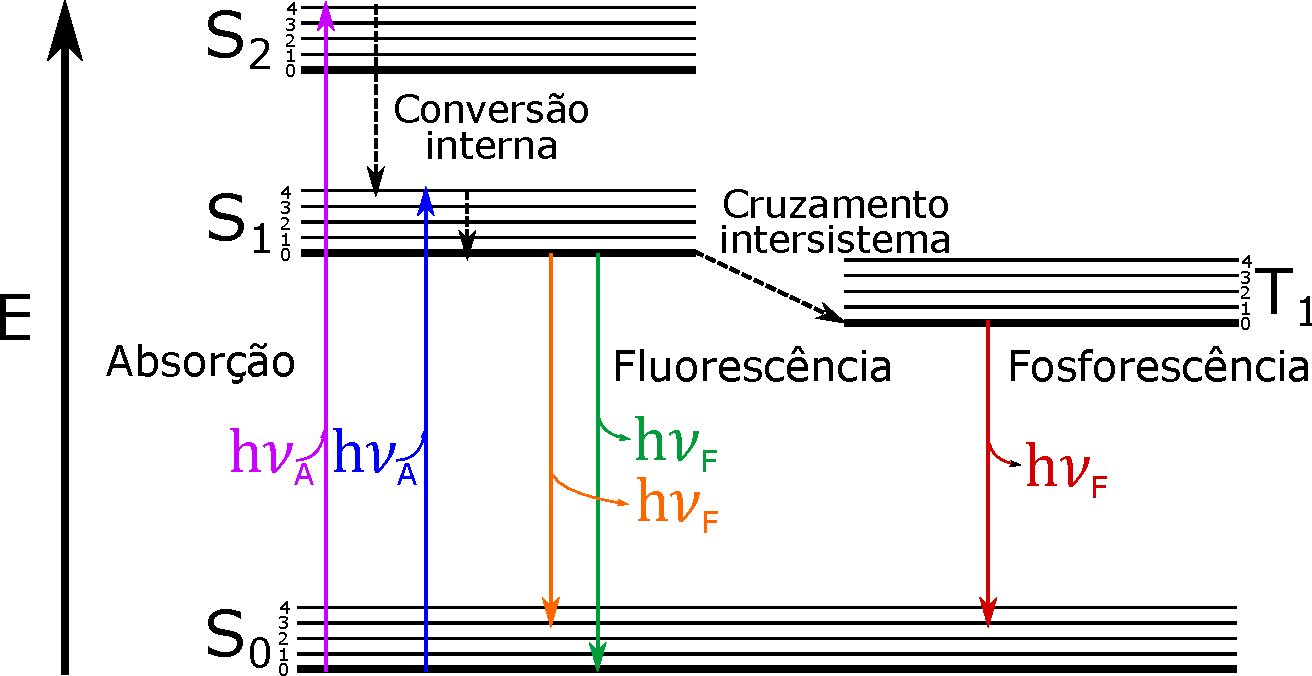
\includegraphics[width=0.7\textwidth]{imagens/fluor/diagrama_jablonski}
			%\caption[Diagrama de Jablonski]{Diagrama de Jablonski. As linhas horizontais indicam níveis energéticos, com níveis mais altos para cima. As setas indicam transições radiativas e as setas tracejadas indicam transições não radiativas. As cores das setas são proporcionais à energia de cada transição. Por simplicidade, não estão representados os fenômenos de extinção, transferência de energia e interação com o solvente. Adaptado de \citeauthor{Lakowicz2006}}
			\caption{Diagrama de Jablonski. As linhas horizontais indicam níveis energéticos, com níveis mais altos para cima. As setas indicam transições radiativas e as setas tracejadas indicam transições não radiativas. As cores das setas são proporcionais à energia de cada transição. Por simplicidade, não estão representados os fenômenos de extinção, transferência de energia e interação com o solvente. Adaptado de \citeauthor{Lakowicz2006}}
			\label{fig:diagrama_jablonski} 
		\end{figure}  
		
		\section{Origem do fenômeno de fluorescência} \index{Fluorescência!origem}
		
		Quando uma molécula absorve radiação no comprimento de onda adequado, um de seus elétrons passa para um nível eletrônico maior, e geralmente para um nível vibracional maior também. Porém, a temperatura ambiente geralmente não é suficiente para manter a molécula vibronicamente excitada, então ela relaxa rapidamente (\(10^{-12}\) s ou menos) para os níveis vibracionais de menor energia do estado eletrônico excitado, um processo chamado de conversão interna. Essa conversão pode ocorrer de estados eletrônicos mais elevados também. Como essa escala de tempo é muito menor do que a de fluorescência (\(10^{-8}\) s), as moléculas excitadas relaxam completamente sua energia vibracional, atingindo um estado eletrônico excitado termicamente equilibrado.\cite{Lakowicz2006}
		
		Após esse equilíbrio térmico, um elétron pode decair para o nível eletrônico fundamental, tanto para níveis vibracionais elevados ou fundamentais, emitindo um fóton de energia igual à transição. Há uma diferença das energias de absorção e de emissão devido à conversão interna e à tendência de ocorrer transições para níveis vibracionais elevados. Essa diferença de energia resulta num deslocamento no comprimento de onda dos espectros de absorção e emissão, chamado de deslocamento de Stokes.\cite{Lakowicz2006} \index{Fluorescência!deslocamento de Stokes}
		
		O fenômeno de conversão interna também implica que o espectro de emissão geralmente é independente do comprimento de onda do fóton incidido, pois o espectro de emissão ocorre sempre do estado vibracional fundamental do estado eletrônico excitado. Essa regra é conhecida como lei de Kasha.\cite{Lakowicz2006} \index{Fluorescência!lei de Kasha}
		
		As transições eletrônicas ocorrem numa faixa de tempo muito rápida, de cerca de \(10^{-15}\) s. Esse tempo é muito rápido para que tenha ocorrido mudanças nas posições dos núcleos. Isso é conhecido como o princípio de Frank-Condon. \index{Fluorescência!princípio de Franck-Condon} Uma das consequências desse princípio é que a probabilidade de uma transição \(S_1 \to S_0\) é igual à probabilidade de uma transição \(S_0 \to S_1\), o que resulta em espectros de emissão e absorção espelhados. Quando o espelhamento não é observado, é possível que o espectro de absorção possua uma absorção para um segundo estado excitado \(S_2\), onde o elétron relaxa rapidamente. Logo, observa-se somente as transições espelhadas entre os estados \(S_1\) e \(S_0\).
			
		As transições para os estados excitados ocorrem sem alteração do spin do elétron. Porém, caso o elétron troque de spin, no fenômeno chamado de cruzamento intersistema, \index{Fluorescência!cruzamento intersistemas} o novo estado, um tripleto, não possui uma transição permitida para o estado singleto fundamental. Isso faz com que as escalas de tempo para a transição sejam muito maiores do que a fluorescência, onde a transição é permitida.
		
		\vfill
		
		\section{Rendimento quântico e tempo de vida} \index{Fluorescência!rendimento quântico}
				
		O rendimento quântico é a eficiência de emissão relativo ao número de fótons absorvidos. Quanto mais próximo de 1 for o rendimento quântico, mais intensa é a fluorescência. O tempo de vida é o tempo em que o fluoróforo permanece em seu estado excitado. Quanto maior for o tempo de vida, mais interações podem ocorrer com moléculas ao redor do fluoróforo, e mais informações podem ser obtidas. \cite{Lakowicz2006}\index{Fluorescência!tempo de vida}
		
		A fluorescência é dependente da polaridade do solvente. \index{Fluorescência!efeito do solvente} Isso ocorre porque, geralmente, o fluoróforo eletronicamente excitado possui um dipolo maior do que no estado fundamental. Isso faz com que as moléculas do solvente ao redor do fluoróforo se rearranjem ao redor dele, diminuindo a energia do sistema, aumentando o deslocamento de Stokes. O rearranjo de uma molécula de solvente ocorre na ordem de 40 ps ou menos, e o rearranjo total ocorre em cerca de \(10^{-10}\) s. Dependendo da polaridade do solvente, os efeitos do rearranjo podem ser maiores ou menores, resultando em deslocamentos de Stokes diferentes e espectros de emissão de fluorescência deslocados.\cite{Lakowicz2006}
		
		Na área de fluorescência existem dois métodos experimentais, a fluorescência estacionária e a fluorescência resolvida no tempo. Na fluorescência estacionária, a amostra é iluminada e observada constantemente. Como os fenômenos de fluorescência são muito rápidos, efetivamente observa-se uma média dos fenômenos que ocorreram durante a observação. Utilizando equipamentos bastante sofisticados, é possível emitir pulsos de radiação curtos e observar o decaimento da fluorescência com o tempo, em escalas de ns. Isso é conhecido como fluorescência resolvida no tempo. Neste trabalho, foi utilizado somente fluorescência estacionária e, de certo modo, uma combinação das duas técnicas, onde observou-se a variação da intensidade de fluorescência em escalas de ms a minutos.\cite{Lakowicz2006}
		
		\section{Extinção} \index{Fluorescência!extinção}
		
		Há fenômenos que conseguem impedir uma molécula de fluorescer, diminuindo a intensidade de fluorescência medido. Esses fenômenos são chamados de extinção (\emph{quenching}). Há pelo menos três mecanismos possíveis para a extinção:
		
		\begin{enumerate}[noitemsep]
			\item Troca eletrônica
			\item Cruzamento intersistemas, ou o efeito do átomo pesado
			\item Transferência eletrônica fotoinduzida.
		\end{enumerate}
		
		Para a extinção ocorrer, é necessário que haja contato entre a molécula do fluoróforo e do \emph{quencher}. \index{Fluorescência!quencher@\textsl{quencher}} Em micelas dopadas com pequenas quantidades de hidrocarbonetos fluorescentes, é observada a extinção pelo íon brometo, mesmo se as duas espécies estão em meios totalmente diferentes, isto é, o brometo está em solução e o hidrocarboneto está no interior das micelas. Uma explicação para esse fenômeno é a formação de canais de água causados pela distorção da estrutura micelar pelos hidrocarbonetos, transportando assim o brometo para a proximidade da sonda, realizando a extinção.\cite{Burrows1980}.
		
		No caso de troca eletrônica, há uma molécula que é pobre eletronicamente, chamada de aceptor e o fluoróforo, o doador. Entrando em contato, o doador transfere seu elétron excitado para o aceptor e recebe de volta um elétron no estado fundamental, concertadamente ou não. Isso equilibra as cargas no sistema, e faz com que o aceptor esteja no estado excitado. O aceptor em seguida pode tanto perder a energia por processos radiativos quanto não-radiativos. \cite{Lakowicz2006}
		
		O cruzamento intersistemas, \index{Fluorescência!cruzamento intersistemas} mecanismo que também dá origem à fosforescência, pode ser induzido por átomos pesados, como halogênios, devido ao acoplamento spin-órbita. Em solução aquosa, um elétron no estado \(T_1\) relaxa por processos não radiativos pois o tempo de vida desse tipo de transição é muito alto. O oxigênio é um \emph{quencher} bastante comum e consegue extinguir a maior parte dos fluoróforos, sendo que em alguns casos é necessário removê-lo do meio para permitir a observação de fluorescência. O mecanismo de atuação do oxigênio ainda é debatido, porém o mais provável é que o oxigênio, paramagnético, causa um cruzamento intersistema, e o sistema depois perde energia não radiativamente. Outros estudos mostram que podem existir vários mecanismos em conjunto atuando, como, além do cruzamento, transferência de carga e troca eletrônica. \cite{Lakowicz2006} 
		
		A transferência eletrônica é resultante da formação de um complexo entre um doador e um aceptor eletrônico (o fluoróforo pode ser ambos), formando um complexo do tipo \(D_p^+A_p^-\), que pode voltar ao estado fundamental sem emissão, porém em alguns casos é observada a emissão desse complexo. Após a relaxação, o elétron é retornado ao doador.  \cite{Lakowicz2006}
				
		Outro parâmetro que pode influenciar a fluorescência é a viscosidade do meio onde o fluoróforo se encontra. \index{Fluorescência!efeito da viscosidade} Isso depende da estrutura e do mecanismo de emissão específico de cada fluoróforo. Por exemplo, uma molécula, conhecida como CCVJ\footnote{9-(2-Carboxi-2-cianovinil)julolidina}, possui um aumento de seu rendimento quântico com o aumento da viscosidade do solvente, em soluções de etileno glicol em glicol. Isso ocorre porque a maior viscosidade atrasa a rotação interna de certos grupos em sua estrutura e dificulta um mecanismo de transferência de carga que extingue a fluorescência, aumentando então o rendimento quântico. \cite{Lakowicz2006}
		
		\section{Aplicações para sistemas micelares}
		
		Na literatura, estudos mostram que a fluorescência, e técnicas correlatas como fluorescência resolvida no tempo, \emph{quenching} resolvido no tempo, são capazes de monitorar a formação de micelas\cite{Zettl2005, Alexandridis1995}, transição de esferas para cilindros e seu crescimento \cite{Vasilescu2004, Goel2010, Gao2011, Almgren1988a, Narayanan1997c}, distribuição de tamanho \cite{Gehlen1993}, formação de micelas com outros formatos\cite{Lima2013b} e dinâmica de solvatação\cite{Kumari2017a, Sen2005}. Geralmente, essas técnicas dependem da adição de um fluoróforo em diminutas quantidades. Porém, o salicilato é fluorescente\cite{ALLISON1964}, e, como será visto, pode ser utilizado como uma sonda para observar o crescimento das micelas, sendo desnecessário adicionar outras sondas, como outros trabalhos tiveram que fazer.\cite{Sen2005, Makhloufi1989}

		
	\chapter{Forças intermoleculares e interagregados} \index{forças intermoleculares} \label{sec:forcas_intermoleculares}
	
	Esta seção se baseia fortemente no excelente livro de Israelachvili, \emph{Intermolecular and Surface Forces}\cite{Israelachvili2011}.
	
	Na natureza existem quatro forças distintas, porém, para o campo dos coloides, a força eletromagnética é de maior importância. As forças comumente estudadas na química, como as interações dipolares e dispersivas, possuem uma origem fundamentalmente eletrostática. De forma geral, potenciais de interação de pares \(w\) podem ser escritos de acordo com
	
	\begin{equation}
		w(r) = -\dfrac{C}{r^n}
		\label{eqn:energia_livre_generica}
	\end{equation} \index{forças intermoleculares!energia livre de interação|textbf}
	
	\noindent onde \(C\) é uma constante de interação, \(r\) é a distância e \(n\) é um fator de distância. A força \(F\) é obtida pela derivada dessa equação em função da posição 
	
	\begin{equation}
		F(r) = -\dfrac{\mathrm{d}w(r)}{\mathrm{d}r} = -n \dfrac{C}{n+1}
		\label{eqn:forca_generica}
	\end{equation} \index{forças intermoleculares!força|textbf}
	
	
	As interações intermoleculares possuem valores de \(n\) entre 4 e 5. Isso permite que não seja necessário considerar o sistema como um todo para calcular as interações intermoleculares, pois as energias de interação decaem rapidamente, sendo efetivas somente em curtas distâncias. Isso não ocorre, por exemplo, para a gravidade, onde as forças ainda são relevantes mesmo a longas distâncias. Mie propôs uma forma para o potencial de interação adicionando um componente repulsivo,
	
	\begin{equation}
		w(r) = -\dfrac{A}{r^n} + \dfrac{B}{r^m}
		\label{eqn:forca_mie}
	\end{equation}
	
	\noindent onde \(A\) e \(B\) são as constantes de interação atrativa e repulsiva, respectivamente, e \(n\) e \(m\) são os fatores de distância. O potencial de Lennard Jones ocorre quando \(n = 6\), \index{forças intermoleculares:potencial de Lennard Jones} correspondente às atrações de van der Waals, e quando \(m = 12\). Os valores comuns de \(A\) e \(B\) são \(10^{-77}\) J e \(10^{-134}\) J.
	
	Quando as interações intermoleculares ocorrem através de um meio, como um solvente, é necessário incluir o efeito das moléculas do solvente nos potenciais de interação. Forças que seriam previamente atrativas podem se tornar repulsivas num solvente, caso a energia necessária para remover as moléculas de solvente exceda a energia de aproximação molecular. Além disso, a presença de moléculas de solvente pode alterar propriedades das moléculas de soluto, como seus momentos de dipolo.
	
	Os valores de energia somente serão úteis se comparados com outros fatores, por exemplo, a energia térmica, que age de modo a equilibrar o sistema e afastar as moléculas. A 1 atm, o valor da energia térmica do solvente é de \(\approx \sfrac{3}{2} k_B T\), onde \(k_B\) é a constante de Boltzmann e \(T\) é a temperatura, então interações com energias menores que \(\sfrac{3}{2}k_BT\) não conseguem so sobrepor ao movimento térmico das moléculas. \index{forças intermoleculares:energia térmica}
	
	As interações intermoleculares possuem três origens distintas:
	
	\begin{enumerate}[noitemsep] 
		\item Origem puramente eletrostática, como no caso de interações entre íons, dipolos (e quadropolos, etc) permanentes, e interações de polarização.
		\item Origem puramente entrópica, que surge do comportamento coletivo das moléculas, como as forças osmóticas.
		\item Origem mecânico quântica, como as ligações covalentes, forças de dispersão de van der Waals, ácido-base, forças estérica repulsivas devido ao princípio de exclusão de Pauli.
	\end{enumerate} \index{forças intermoleculares:origens}
	
	\section{Interações Coulombicas} \index{forças intermoleculares: coulombicas}
	
	As interação Coulombica depende do campo elétrico entre uma partícula carregada e a carga de outra partícula próxima. O campo elétrico é dado pela \autoref{eqn:campo_eletrico}.
	
	\begin{equation}
		E = \dfrac{Q_1}{4\pi\varepsilon_0\varepsilon r^2}
		\label{eqn:campo_eletrico}
	\end{equation} \index{forças intermoleculares!campo elétrico}

	\noindent onde \(Q_1\) é a carga da partícula, \(\varepsilon_0\) é a constante dielétrica do vácuo e \(\varepsilon\) é a constante dielétrica relativa do meio em questão. \index{forças intermoleculares:constante dielétrica} Como pode ser visto, a presença de um meio diminui a força da interação eletrostática por \(\varepsilon\), então em solventes com constantes dielétricas altas, a força eletrostática é bastante enfraquecida. É necessário enfatizar que os termos \(\varepsilon\) e \(\varepsilon_0\) são dependentes da frequência \(\nu\) do campo elétrico aplicado (por exemplo, o campo elétrico oscilatório da luz). Em frequência zero, em condições estáticas, esses termos recebem o nome de constante dielétrica, mas fora dessas condições recebem o nome de permissividade elétrica. \index{forças intermoleculares!constante dielétrica!dependência com a frequência}
	
	O potencial de interação entre cargas é obtido pelo processo oposto da \autoref{eqn:forca_generica}, ou seja, pela integração da força eletrostática, dada por \(F = Q_2 E\) (\autoref{eqn:potencial_eletrostático}), utilizando o estado de referência das cargas como sendo no infinito.
	
	\begin{equation}
		w(r) = \int_\infty^r -F(r)dr = \dfrac{z_1z_2e^2}{4\pi\varepsilon_0\varepsilon r}
		\label{eqn:potencial_eletrostático}
	\end{equation} \index{forças intermoleculares!energia eletrostática|textbf}
	
	Interessantemente, a força gravitacional e a interação Coulombica são comparáveis pois possuem um potencial da forma \(1/r\), portanto são de longo alcance, e também são aditivas, isto é, a interação entre dois corpos não é dependente da presença de outros corpos ao redor. Esse conceito é importante, pois as interações dispersivas, de grande relevância para coloides, não são aditivas.
	
	\section{Interações dipolares} \index{forças intermoleculares!dipolares}
	
	A maioria das moléculas não possui uma carga, mas sim um momento de dipolo, resultante da posição de cargas totais ou parciais em diferentes pontos da molécula. O momento de dipolo é definido como
	
	\begin{equation}
		u = ql
		\label{eqn:momento_dipolo}
	\end{equation} \index{forças intermoleculares!momento de dipolo}
	
	\noindent onde \(u\) é o momento de dipolo e \(l\) é a separação entre as cargas \(+q\) e \(-q\). Essas cargas não precisam estar alinhadas, sendo necessário então corrigir esse não alinhamento pela soma vetorial dos momentos de dipolo individuais.
	
	A energia de interação entre duas moléculas dipolares (sendo uma delas fixa) é dada por
	
	\begin{equation}
		w \left( r , \theta _ { 1 } , \theta _ { 2 } , \phi \right) = - \frac { u _ { 1 } u _ { 2 } } { 4 \pi \varepsilon \varepsilon _ { 0 } r ^ { 3 } } \left[ 2 \cos \theta _ { 1 } \cos \theta _ { 2 } - \sin \theta _ { 1 } \sin \theta _ { 2 } \cos \phi \right]
		\label{eqn:energia_dipolo_dipolo}
	\end{equation} \index{forças intermoleculares!energia dipolar}
	
	\noindent onde \(\theta_{ 1 }\) e \(\theta_{ 2 }\) são os ângulos das duas moléculas dipolares em relação à reta que as liga, \(\phi\) é o ângulo de rotação perpendicular a \(\theta_{ 2 }\) de uma das moléculas. É interessante ver que essa interação também é dependente da constante dielétrica, além de ser dependente de \(r^{-3}\).  % todo: pensar se eu devo deixar essa equação ou só colocar a de Keesom
	
	Se os dois dipolos puderem rodar livremente, a energia média dessa interação, conhecida como energia de Keesom é dada por
	
	\begin{equation}
		w(r) = - \dfrac{u _ { 1 } ^ { 2 } u _ { 2 } ^ { 2 } }{ 3 \left( 4 \pi \varepsilon \varepsilon _ { 0 } \right) ^ { 2 } k_B T r ^ { 6 } }
		\label{eqn:energia_Keesom}
	\end{equation} \index{forças intermoleculares!energia dipolar|textbf} \index{forças intermoleculares!Keesom|see {energia dipolar}}
	
	Note que aqui, a dependência com a distância é da ordem de \(r^{-6}\). Essa é uma das componentes das interações de van der Waals. \index{forças intermoleculares!curto alcance}
	
	\section{Interações de polarização} \index{forças intermoleculares!polarização}
	
	Átomos ou moléculas submetidos a um campo elétrico se alinham no sentido contrário ao campo. A magnitude desse alinhamento é dependente da polarizabilidade das moléculas, \(\alpha\), e da intensidade do campo, \(E\),
	
	\begin{equation}
		u_{\mathrm{ind}} = \alpha E
		\label{eqn:dipolo_induzido}
	\end{equation} \index{forças intermoleculares!dipolo induzido}
	
	A polarizabilidade do material é composta por uma componente devido ao dipolo inerente da molécula, se houver, e outra componente sempre presente, que aparece devido à distorção da nuvem eletrônica dos átomos ou moléculas, chamada de polarizabilidade eletrônica, \(\alpha_0\). \index{forças intermoleculares!polarizabilidade eletrônica}
	
	A equação de Debye-Langevin (\autoref{eqn:debye_langevin}) relaciona a polarizabilidade total com a polarizabilidade eletrônica e o momento de dipolo.
	
	\begin{equation}
		\alpha = \alpha _ { 0 } + \dfrac{u ^ { 2 }}{ 3 k_B T }
		\label{eqn:debye_langevin}
	\end{equation} \index{forças intermoleculares!relação entre polarizabilidade total e polarizabilidade eletrônica}
	
	Uma maneira de se visualizar essa polarização é considerando um átomo de hidrogênio de Bohr. Quando esse átomo é colocado em um campo elétrico, a posição relativa do elétron e do próton configura um dipolo, que irá interagir com o campo, apesar de que o átomo não possui um momento de dipolo permanente.
	
	Uma consequência da polarização das moléculas é justamente a constante dielétrica \index{forças intermoleculares!constante dielétrica|textbf}, que é medida colocando-se o material entre duas placas carregadas de um capacitor. Devido ao campo elétrico, as moléculas alinham seus dipolos, naturais e induzidos, contrariamente ao campo. A soma desses dipolos alinhados gera um campo contrário ao campo aplicado \(E_0\), diminuindo o campo efetivo \(E\). A razão \(\sfrac{E_0}{E}\) resulta na constante dielétrica do meio. Quanto maior for a polarização, maior é a queda do campo efetivo, e maior é a constante dielétrica. Há solventes que possuem mecanismos adicionais para gerar polarização, como o deslocamento de cargas por distâncias significativamente maiores que os tamanhos moleculares. Um exemplo disso é a água, onde elétrons ou prótons são transportados pelas ligações de hidrogênio,\cite{Israelachvili2011} e amidas secundárias, cujos valores de constante dielétrica podem chegar até 180.\cite{ReichardtSolvents}

	Outra consequência da polarização de moléculas é o surgimento de uma força entre os dipolos permanentes e dipolos induzidos, chamada de interação de Debye, cujo potencial de energia é dado por
	
	\begin{equation}
		w ( r ) = - \frac { \left[ u _ { 1 } ^ { 2 } \alpha _ { 02 } + u _ { 2 } ^ { 2 } \alpha _ { 01 } \right] } { \left( 4 \pi \varepsilon _ { 0 } \varepsilon \right) ^ { 2 } r ^ { 6 } }
		\label{eqn:energia_Debye}
	\end{equation} \index{forças intermoleculares!dipolo permanente e dipolo induzido} \index{forças intermoleculares!Debye|see {dipolo induzido}}
	
	\noindent onde os subíndices \emph{1, 2} indicam as propriedades (momentos de dipolo \(u\) e polarizabilidades eletrônicas \(\alpha_0\)) de duas moléculas/átomos diferentes. Da mesma maneira que a energia de Keesom (\autoref{eqn:energia_Keesom}), a dependência da energia de Debye é proporcional a \(r^{-6}\). \index{forças intermoleculares!curto alcance}
	
	Quando moléculas estão em um meio composto por outras moléculas também com polarizabilidade eletrônica definida, \index{forças intermoleculares!efeito do solvente} as polarizabilidades de excesso se tornam relevantes, ou seja, é a diferença entre a polarizabilidade de uma molécula com a polarizabilidade natural do meio. Essa abordagem assume que as propriedades são contínuas, o que apresenta suas limitações quando as distâncias de interação são bastante curtas. A \autoref{eqn:polarizabilidade_excesso} mostra como a polarizabilidade de uma molécula esférica \(i\), com constante dielétrica \(\varepsilon_i\) e volume \(v_i\), é afetada ao estar num meio de constante dielétrica \(\varepsilon\). \index{forças intermoleculares!polarizabilidade de excesso}
	
	\begin{equation}
		\alpha_i = 3 \varepsilon_{ 0 } \varepsilon \left( \dfrac{\varepsilon_i - \varepsilon}{\varepsilon_i + 2 \varepsilon}  \right) v_i
		\label{eqn:polarizabilidade_excesso}
	\end{equation}
	 
	 Essa equação pode ser utilizada para descobrir a polarizabilidade total de uma molécula no estado gasoso (onde \(\varepsilon = 1\)), relação conhecida como a equação de Clausius-Mossotti (\autoref{eqn:clausius_mossotti})\cite{Rysselberghe1931, Atkins2017}.
	 \index{forças intermoleculares!Clausius-Mossotti|see{relação entre polarizabilidade e constante dielétrica}} \index{forças intermoleculares!relação entre polarizabilidade e constante dielétrica}
	 
	 \begin{equation}
		\dfrac { \alpha } { \left( 4 \pi \varepsilon _ { 0 } \right) } = \left( \dfrac { \varepsilon - 1 } { \varepsilon + 2 } \right) \dfrac { 3 v } { 4 \pi }
		\label{eqn:clausius_mossotti}
	 \end{equation}
	
	A polarizabilidade eletrônica \(\alpha_0\) pode ser calculada por uma modificação da equação de Clausius-Mossotti. Ao invés de se utilizar as constantes dielétricas, onde a frequência de perturbação é zero, é necessário utilizar as permissividades na frequência do UV-visível. Na região do UV-visível, o índice de refração, definido na \autoref{eqn:def_n}, se relaciona diretamente com a permissividade elétrica (\autoref{eqn:permissividade_e_indice_refrac}).\cite{Atkins2017}
	
	\begin{equation}
		\varepsilon(\nu) = n(\nu)^2
		\label{eqn:permissividade_e_indice_refrac}
	\end{equation} \index{forças intermoleculares!relação entre constante dielétrica e índice de refração}
	
	\begin{equation}
		n = \dfrac{c_0}{c}
		\label{eqn:def_n}
	\end{equation} \index{forças intermoleculares!índice de refração|textbf}
	
	\noindent onde \(n\) é o índice de refração, \(c_0\) é a velocidade da luz no vácuo e \(c\) é a velocidade da luz no meio.
	
	Com isso, pode-se obter a equação de Lorenz-Lorentz, \autoref{eqn:lorenz_lorentz},\cite{Israelachvili2011} que relaciona a polarizabilidade eletrônica com o índice de refração. Em frequências altas, acima de \(10^{12}\) Hz, dipolos moleculares não possuem tempo suficiente para responder a um campo, então a polarização é devido somente à polarização eletrônica. Essa separação de comportamentos a frequência zero e frequência no UV-Vis, utilizando a constante dielétrica e o índice de refração ocorrerá em outras equações desta seção.
	
	\begin{equation}
		\dfrac { \alpha _ { 0 } } { \left( 4 \pi \varepsilon _ { 0 } \right) } = \left( \dfrac { n ^ { 2 } - 1 } { n ^ { 2 } + 2 } \right) \dfrac { 3 v } { 4 \pi }
		\label{eqn:lorenz_lorentz}
	\end{equation} \index{forças intermoleculares!lorenz-lorentz|see{relação entre polarizabilidade eletrônica e índice de refração}} \index{forças intermoleculares!relação entre polarizabilidade eletrônica e índice de refração}

	\section{Forças de van der Waals}  \index{forças intermoleculares!van der Waals}
	
	As forças de van der Waals são compostas pelas forças dispersivas, junto com as forças de Keesom e Debye. Esse nome vem da dispersão da luz na região do visível e ultravioleta. As forças dispersivas são as mais importantes das três forças, pois estão presentes em todas as moléculas e átomos, podem ser de longa distância, atrativas ou repulsivas, e não são aditivas.
	
	A origem das forças dispersivas está na eletrodinâmica quântica, porém sua natureza ainda é essencialmente eletrostática. Um átomo ou molécula não polar possui momento de dipolo temporal médio igual a zero, mas, como mencionado para o átomo de hidrogênio de Bohr, a cada momento existe um momento de dipolo devido à disposição da nuvem eletrônica ao redor do núcleo. Esse momento de dipolo instantâneo irá induzir um momento de dipolo num átomo vizinho, e estes irão interagir eletrostaticamente. A média temporal dessa atração é não nula, apesar da média temporal dos momentos de dipolo ser nula. O momento de dipolo instantâneo do átomo de hidrogênio de Bohr é de 2,5 Debye, o que não é pequeno.
	
	A energia de interação de van der Waals entre dois átomos, 1 e 2,  no vácuo pode ser descrita pela \autoref{eqn:energia_dispersiva}, proposta por London em 1937.\cite{London1937}
	
	\begin{equation}
		w(r) = - \frac { 3 } { 2 } \frac { \alpha _ { 01 } \alpha _ { 02 } } { \left( 4 \pi \varepsilon _ { 0 } \right) ^ { 2 } r ^ { 6 } } \frac { h \nu _ { 1 } \nu _ { 2 } } { \left( \nu _ { 1 } + \nu _ { 2 } \right) }
		\label{eqn:energia_dispersiva}
	\end{equation} \index{forças intermoleculares!dispersiva}
	
	\noindent onde \(h\) é a constante de Planck e \(\nu\) é a frequência de absorção do átomo. O termo \(h\nu_i\) pode ser substituído por \(I_i\), a energia de ionização do átomo \(i\). É possível notar a dependência de \(r^{-6}\) que as outras energias também possuem. Essa equação assume que há somente uma absorção eletrônica. \index{forças intermoleculares!curto alcance}
	
	Agora que o terceiro componente foi definido, é possível obter o panorama completo da energia de interação de van der Waals obtido pela soma das três energias,
	
	\begin{subequations}
	\begin{align}
		w_{\mathrm{VDW}}(r) &= -C_{\mathrm{VDW}}/r^{6} = -\left[C_{\mathrm{Debye}}+C_{\mathrm{Keesom}}+C_{\mathrm{London}}\right]/r^{6} \label{eqn:vdw_geral} \\
							&= - \left[ \left( u_{1}^{2}\alpha_{02} + u_{2}^{2}\alpha_{01} \right)   + \frac{u_{1}^{2}u_{2}^{2}}{3k_BT} + \frac{3\alpha_{01}\alpha_{02}h\nu_{1}\nu_{2}}{2\left(\nu_{1} + \nu_{2}\right)}\right]/\left(4\pi\varepsilon_{0}\right)^{2}r^{6} \label{eqn:vdw_completa}
	\end{align}
	\label{eqn:vdw}
	\end{subequations} \index{forças intermoleculares!curto alcance}
	
	Porém, essa equação possui algumas limitações. Não são consideradas absorções além da primeira absorção eletrônica, e não é possível levar em consideração o meio. MacLachlan utilizou uma somatória de todas as possíveis absorções para expandir a abrangência da equação, e utilizou propriedades de excesso de um sistema contínuo para poder considerar a presença de um meio. Assumindo que todos os meios possuem a mesma energia de absorção, e que as partículas \emph{1} e \emph{2} sejam iguais e dispersas no meio \emph{3}, é possível obter a \autoref{eqn:energia_maclachlan}, onde as contribuições estáticas, onde \(\nu = 0\) (Debye e Keesom) foram separadas das contribuições de frequências altas, onde predominam as interações dispersivas.
	
	\begin{equation}
		w ( r ) = w ( r ) _ { \nu = 0 } + w ( r ) _ { \nu > 0 } \approx - \left[ 3 k_B T \left( \frac { \varepsilon _ { 1 } ( 0 ) - \varepsilon _ { 3 } ( 0 ) } { \varepsilon _ { 1 } ( 0 ) + 2 \varepsilon _ { 3 } ( 0 ) } \right) ^ { 2 } + \frac { \sqrt { 3 } h \nu _ { e } } { 4 } \frac { \left( n _ { 1 } ^ { 2 } - n _ { 3 } ^ { 2 } \right) ^ { 2 } } { \left( n _ { 1 } ^ { 2 } + 2 n _ { 3 } ^ { 2 } \right) ^ { 3 / 2 } } \right] \frac { a _ { 1 } ^ { 6 } } { r ^ { 6 } }
		\label{eqn:energia_maclachlan}
	\end{equation} \index{forças intermoleculares!expansão de MacLachlan}
	
	\noindent onde \(a_1\) é o raio da molécula 1.
	
	Alguns fatores podem ser levantados sobre essa equação. Geralmente, a componente com \(\nu > 0\) é mais forte que a componente com \(\nu = 0\), exceto em solventes polares, como a água. Além disso, a força de van der Waals é reduzida num meio com solvente, devido às propriedades de excesso serem menores do que no vácuo. Por último, a força dispersiva é sempre atrativa entre moléculas iguais\cite{Hamaker1937}, mas a expressão expandida mostra que as interações podem ser tanto atrativas quanto repulsivas, quando a propriedade do solvente, como o índice de refração, é intermediário entre as duas partículas. Uma maneira de se visualizar isso é pensando no princípio de Arquimedes. A força gravitacional é, aparentemente, sempre atrativa. Porém, ao colocar uma esfera de isopor no fundo de uma banheira, a esfera irá subir para a superfície, sendo que uma esfera de aço afundaria. A causa da repulsão da esfera de isopor é a força gravitacional, que agiu com maior força no volume de água deslocado pelo isopor do que na própria esfera de isopor, e a deslocou para cima. \index{forças intermoleculares!repulsão}
	
	\section{Ligações de hidrogênio e interações hidrofóbicas} \index{forças intermoleculares!ligação de hidrogênio} \index{forças intermoleculares!interação hidrofóbica} \label{sec:ligacoes_hidrogenio}
	
	Na molécula de água, há uma grande diferença de eletronegatividade entre O e H, resultando numa grande polarização dessa ligação. A molécula de água pode ser representada centrada no oxigênio, com duas cargas positivas nos hidrogênios e duas cargas negativas nos pares eletrônicos do oxigênio. Essa interação entre as regiões positiva e negativa das moléculas de água, de natureza eletrostática, é bastante forte, da ordem de 5-10 \(k_BT\) a 298K. Essa interação pode ser visualizada através das distâncias de ligação, onde a ligação intramolecular O --- H é de 0.10 nm, a distância intermolecular \(\mathrm{O} \cdots \mathrm{H}\) é 0.176 nm, e a soma dos raios de van der Waals de O e H é de 0.26 nm. Devido à essa forte interação, as moléculas de água formam uma estrutura tetraédrica, com quatro moléculas de água ao redor, no estado sólido, e uma média de 3,5 moléculas de água no estado líquido, ao invés de 12 moléculas para estruturas com empacotamento denso.
	
	A forte tendência da água de formar ligações de hidrogênio influencia quando algum soluto grande, que não consegue realizar ligações de hidrogênio, é adicionado. Não importa a disposição das moléculas de água, haverá alguma das cargas parciais que não conseguirá ser totalmente equilibrada. Uma consequência disso é o aparecimento de cargas negativas em superfícies hidrofóbicas, pois moléculas de água se direcionam preferencialmente com o oxigênio em direção à essas superfícies, ocorrendo um acúmulo das cargas negativas parciais. Outra consequência é que em solutos hidrofóbicos, como hidrocarbonetos longos, causam uma estruturação da água envolvendo o hidrocarboneto, que é entropicamente desfavorável, já que rompe a estrutura existente e impõe uma estrutura ordenada. Por exemplo, a interação entre n-butano e água é entalpicamente favorável (\(\Delta H = -4,3\) kJ.mol\menosUm), porém é extremamente entropicamente desfavorável (\(-T\Delta S = +28,7\) kJ.mol\menosUm), resultando no \(\Delta G_{\mathrm{transferência}} = +24.5\) kJ.mol\menosUm. Essa energia é proporcional à área da superfície hidrofóbica, e é próxima à tensão superficial de água e um hidrocarboneto. \index{forças intermoleculares!interação de hidrocarbonetos com água}
	
	A interação hidrofóbica é o nome dado à força de atração entre espécies hidrofóbicas em água, que é muito maior à força de atração daquelas em vácuo, devido ao efeito hidrofóbico. Quando duas moléculas solvatadas se aproximam, suas esferas de hidratação se sobrepõem, e moléculas de água se tornam livres. Do lado oposto, a interação hidrofílica resulta na repulsão de espécies em água, e ocorre em materiais conhecidos por absorver água do ar, isto é, higroscópicos.
	
	O efeito de certos solutos em água pode, então, tanto estruturar quanto desestruturar as moléculas de água locais. Os agentes que desestruturam água são chamados de agentes caotrópicos, e são geralmente hidrofílicos. Por outro lado, agentes que estruturam a água são chamados de agentes cosmotrópicos. Mais informações sobre esse tema podem ser encontrados em \citeauthor{Marcus2009a} % todo: para a defesa, ler mais sobre isso.
	\index{forças intermoleculares!caotrópico} \index{forças intermoleculares!cosmotrópico} \index{forças intermoleculares!desestruturação do solvente} \index{forças intermoleculares!estruturação do solvente}
	
	
	% Polarizabilidade de excesso
	% \alpha _ { 1 } ( \nu ) = 4 \pi \varepsilon _ { 0 } \varepsilon _ { 3 } ( \nu ) \left( \frac { \varepsilon _ { 1 } ( \nu ) - \varepsilon _ { 3 } ( \nu ) } { \varepsilon _ { 1 } ( \nu ) + 2 \varepsilon _ { 3 } ( \nu ) } \right) a _ { 1 } ^ { 3 }
	\section{Coloides e atração coloidal} \index{forças intercoloidais}
	\label{sec:coloides_atracao_coloidal}
	Coloides são sistemas onde há uma dispersão de partículas em solução, onde pelo menos uma das dimensões das partículas está na faixa de 5 nm a 100 \(\mu\)m. Coloides podem ser tanto termodinamicamente estáveis, como podem ser instáveis mas com um tempo de vida muito grande. Como exemplos de coloides temos micelas, moléculas poliméricas e emulsões.\cite{Cosgrove2009, Israelachvili2011}
	
	Para calcular as interações entre duas partículas, é necessário calcular as atrações e repulsões entre todas as moléculas de uma partícula com todas as moléculas da outra partícula. Logo, as energias se tornam proporcionais ao tamanho das partículas. \index{forças intercoloidais!origem}
	
	Outro fator importante são as dimensões em estudo. As propriedades de gases e fases condensadas são determinadas principalmente pela energia de interação quando as partículas estão em contato. No caso de coloides, a situação se altera, e as interações principais são as de longo alcance. Além disso, quando as partículas são ``moles'' (do inglês \emph{soft}), isto é, não possuem uma estrutura rígida, as interações se tornam dependentes dos formatos transientes de ambas as partículas, como, por exemplo, as forças de ondulação de bicamadas. No total, as interações entre coloides são quantitativamente, e qualitativamente, diferentes daquelas de moléculas pequenas.
	\index{forças intercoloidais!efeito do tamanho}
	
	Como uma aproximação inicial, é possível calcular as interações de van der Waals entre partículas com diversos formatos, assumindo que as forças são aditivas. Por exemplo, a interação de van der Waals possui energia \(w(r) = C/r^6\) (\autoref{eqn:vdw_geral}), mas a interação de van der Waals entre duas esferas de tamanhos coloidais de raios \(R_1\) e \(R_2\) separadas por uma distância \(D\) é dado pela \autoref{eqn:interacao_duas_esferas}. \index{forças intercoloidais!aditividade}
	
	\begin{equation}
		w(D) = \dfrac{-A}{6D} \left( \dfrac{R_1R_2}{R_1 + R_2}   \right)
		\label{eqn:interacao_duas_esferas}
	\end{equation}
	
	\noindent onde \(A\) é a constante de Hamaker, conceitualmente semelhante à constante \(C\) das interações entre moléculas. A constante de Hamaker é definida pela \autoref{eqn:constante_hamaker}. \index{forças intercoloidais!constante de Hamaker}
	
	\begin{equation}
		A = \pi^2 C \rho_1 \rho_2
		\label{eqn:constante_hamaker}
	\end{equation}
	
	\noindent onde \(C\) é a constante de interação de van der Waals, \(\rho\) é a densidade numérica das partículas \emph{1, 2}. Valores típicos de \(A\) são da ordem de \(10^{-19}\) J, para \(C = 10^{-77}\) J.m\(^6\) e \(\rho=3 \times 10^{28}\) m\(^{-3}\).
	
	É interessante notar a grande divergência entre a energia de interação de van der Waals entre moléculas quanto à sua dependência com a distância. Enquanto a interação intermolecular tem dependência de \(r^{-6}\), a interação interpartícula tem dependência de \(D^{-1}\), parecida com a força gravitacional, caracterizando seu longo alcance.
	\index{forças intercoloidais!longo alcance}
	\index{forças intercoloidais!aditividade|textbf}

	Porém, a suposição de que as interações de van der Waals são aditivas é falsa. Isso ocorre porque quando um átomo 1 interage com um átomo 2 e um átomo 3, todos próximos, a polarização de 1 em 2 ocorrerá tanto diretamente, como também através da polarização de 1 em 3, que por sua vez irá polarizar 2. Logo, houve uma ``reflexão'' da polarização de 1 pelo átomo 3. Para resolver esse problema, Lifshitz \index{forças intercoloidais!teoria de Lifshitz} criou uma teoria onde a estrutura atômica é ignorada, e as interações são descritas somente pelas propriedades do \emph{bulk}, como índices de refração e constantes dielétricas, semelhante à \autoref{eqn:energia_maclachlan}. Com essa teoria, é possível calcular constantes de Hamaker sem o efeito de retardação (definido em breve), mas considerando a aditividade. Para o caso onde há duas partículas 1 interagindo num meio 3, a constante de Hamaker possui a forma da \autoref{eqn:constante_hamaker_lifshitz}. Como a teoria de Lifshitz se baseia na teoria do contínuo, a separação dos materiais interagentes deve ser maior do que as dimensões moleculares.
	
	\begin{equation}
	A = A_{\nu=0} + A_{\nu>0}  = \frac{3}{4} k_BT \left( \frac { \varepsilon_{1}-\varepsilon_{3}} { \varepsilon_{1} + \varepsilon_{3} } \right)^{2} + \frac{3h\nu_{\mathrm{e} } } {16\sqrt{2}} \frac{\left(n_{1}^{2} - n_{3}^{2} \right)^{2}} {\left(n_{1}^{2} + n_{3}^{2} \right)^{3/2} }
	\label{eqn:constante_hamaker_lifshitz}
	\end{equation} \index{forças intercoloidais!constante de Hamaker}
	
	\noindent onde \(\nu_e\) é a frequência da primeira absorção eletrônica dos componentes, geralmente \(3 \times 10^{15}\) s\menosUm.
	
	Da mesma maneira que na equação de MacLachlan (\autoref{eqn:energia_maclachlan}), a constante de Hamaker pode ser dividida em duas componentes, uma relativa aos dipolos, nunca maior que \(\sfrac{3}{4}k_BT\), e uma componente relativa às interações dispersivas, geralmente mais relevante. Como visto anteriormente, as forças entre duas partículas iguais serão sempre atrativas, porém a magnitude da atração diminui à medida que os índices de refração do solvente e das partículas se tornam parecidos. Esse princípio será essencial para entender os estudos reológicos apresentados neste trabalho.
	
	Um caso onde a contribuição em frequência zero é relevante é na interação de hidrocarbonetos e água, devido principalmente à alta constante dielétrica da água. Nesse caso, \(A = A_{\nu=0} + A_{\nu>0} = (0,28 + 0,17) \times 10^{-20} \) J a 300 K, ou seja, a contribuição dos dipolos é mais do que 50\% da contribuição total da atração, o que pode ser visualizado como uma consequência do efeito hidrofóbico.
	
	\index{forças intercoloidais!efeitos de retardação}
	Ambas contribuições da constante de Hamaker podem ser reduzidas com a distância. O termo \(A_{\nu > 0}\) é reduzido pelos efeitos de retardação (\emph{Retardation Effects}), que se tornam relevantes além de distâncias de 5 nm. Nesse caso, ao invés da energia depender de \(r^{-1}\), começa a depender de \(r^{-2}\). Esses efeitos são consequência do tempo de propagação da força e a frequência de oscilação de dipolos induzidos, que pode ter mudado de configuração no tempo que a energia foi propagada para interagir.
	
	Por outro lado, o termo \(A_{\nu = 0}\) não é afetado pelos efeitos de retardação, mas é dependente da blindagem por íons em soluções aquosas. Nesse caso, o decaimento é exponencial, dependendo do comprimento de blindagem de Debye. Para um eletrólito 1:1, o comprimento de Debye \(1/\kappa\) é dado pela \autoref{eqn:comprimento_debye}.
	
	\begin{equation}
		1/\kappa = \dfrac{0{,}304}{\sqrt{\left[ \mathrm{Eletrólito} \right] }} \textrm{nm}
		\label{eqn:comprimento_debye}
	\end{equation} \index{forças intercoloidais!comprimento de Debye}
	
	Logo, para uma solução 0,1 mol.L\menosUm{} de NaCl possui um comprimento de Debye de aproximadamente 1 nm. A 2 nm, as forças eletrostáticas são da ordem de 13\% do valor inicial.
	
	Relacionado ao comprimento de Debye, há o comprimento de Bjerrum, que relaciona a distância onde a energia Coulombica entre duas cargas se iguala à energia térmica (\autoref{eqn:comprimento_bjerrum}).
	
	\begin{equation}
		\lambda_B = \dfrac{e^2}{4 \pi \varepsilon_{ 0 } \varepsilon k_BT}
		\label{eqn:comprimento_bjerrum}
	\end{equation} \index{forças intercoloidais!comprimento de Bjerrum}
	
	Em soluções aquosas, coloides podem adquirir carga devido à ionização ou dissociação de grupos superficiais, adsorção de íons da solução, ou mecanismos de troca de carga do tipo ácido-base. A carga superficial de íons é contrabalanceada por uma região de contraíons, sendo que parte estão ligados, transientemente, à superfície, na chamada camada de Stern. \index{forças intercoloidais!camada de Stern} Outros íons mais distantes à superfície em movimento térmico configuram a dupla camada elétrica difusa, que se estende até o comprimento de Debye a partir da superfície do coloide. A distribuição de íons é dada pela equação de Poisson-Boltzmann.
	
	A maior parte dos contraíons que efetivamente contrabalanceiam a carga está muito próxima à superfície, a uma distância de poucos \aa ngstrom. Logo, a repulsão entre duas superfícies carregadas num solvente tem origem entrópica (osmótica), não eletrostática. Quando as duas superfícies se aproximam, os contraíons da solução, que estão longe das superfícies por efeitos entrópicos, são forçados à retornar à superfície, perdendo liberdade conformacional, contrariando a força osmótica.
	
	A energia de interação de dupla camada elétrica para duas partículas esféricas de raios \(R_1\) e \(R_2\) a uma distância \(D\) é dada por
	
	\begin{equation}
		w(D) = \left(  \dfrac{R_1R_2}{R_1+R_2}  \right)Ze^{-\kappa D}
		\label{eqn:dupla_camada_esferas}
	\end{equation} \index{forças intercoloidais!dupla camada elétrica}
	
	\noindent onde \(Z\) é uma constante de interação análoga à constante de Hamaker, definida como 
	
	\begin{equation}
		Z = 64 \pi \varepsilon _ { 0 } \varepsilon ( k_B T / e ) ^ { 2 } \tanh ^ { 2 } \left( z e \psi _ { 0 } / 4 k_B T \right)
		\label{eqn:constante_interacao_Z}
	\end{equation} \index{forças intercoloidais!constante de interação Z}
	
	\noindent onde \(z\) é a valência do eletrólito (\(z=1\) para NaCl), \(e\) é a carga do elétron e \(\psi_0\) é o potencial de superfície.
	
	A combinação das forças de van der Waals com as forças de dupla camada elétrica descreve as interações entre coloides. A teoria DLVO foi nomeada em homenagem aos seus criadores (Derjaguin, Landau, Verwey, Overbeek). Essa teoria consegue prever, através do equilíbrio entre as energias de van der Waals atrativas e as energias repulsivas de dupla camada, vários fenômenos coloidais, como a estabilidade cinética, coagulação/floculação e repeptização. Além das forças da teoria de DLVO, ainda há forças de solvatação, estruturais, hidratação, estéricas e ondulação. \index{forças intercoloidais!teoria DLVO}
	

	\chapter{Micelas gigantes} \index{micelas gigantes|textbf}
	% todo: Falar sobre os tempos de relaxação vistos por Hoffmann por birrefringência elétrica
	Este capítulo irá contextualizar a teoria vista nos capítulos anteriores para o campo de micelas gigantes, e expandir em algumas áreas. Excelentes livros e artigos introdutórios podem ser encontrados nas referências \cite{Dreiss2007, Giant_Micelles, WLM_Advances, Herb1994, Ezrahi2006}.

		\label{chap:micelas_gigantes}
		\section{Estruturas e tamanhos}  % todo: rever esse nome
		\index{micelas gigantes!estrutura}
		Como mencionado no \autoref{sec:surfactantes_autoassociação}, micelas gigantes são formadas por moléculas de surfactante. O parâmetro de empacotamento dessas moléculas pode ser alterado pela adição de mais surfactante, sais inorgânicos, sais orgânicos (hidrótropos\footnote{Sais anfifílicos mas com uma região apolar pequena}), cosurfactantes pequenos, surfactantes não iônicos, pela mistura de surfactantes catiônicos e aniônicos, ou também pela alterações nas características do solvente, como sua temperatura e pH.\cite{Dreiss2007} A alteração do parâmetro de empacotamento leva a mudanças na curvatura micelar, que acaba levando à formação de estruturas diferentes. A \autoref{fig:regimes_e_estruturas_lequeux} mostra um diagrama de fase esquemático para estruturas alongadas.
		
		\begin{figure}[h]
			\centering
			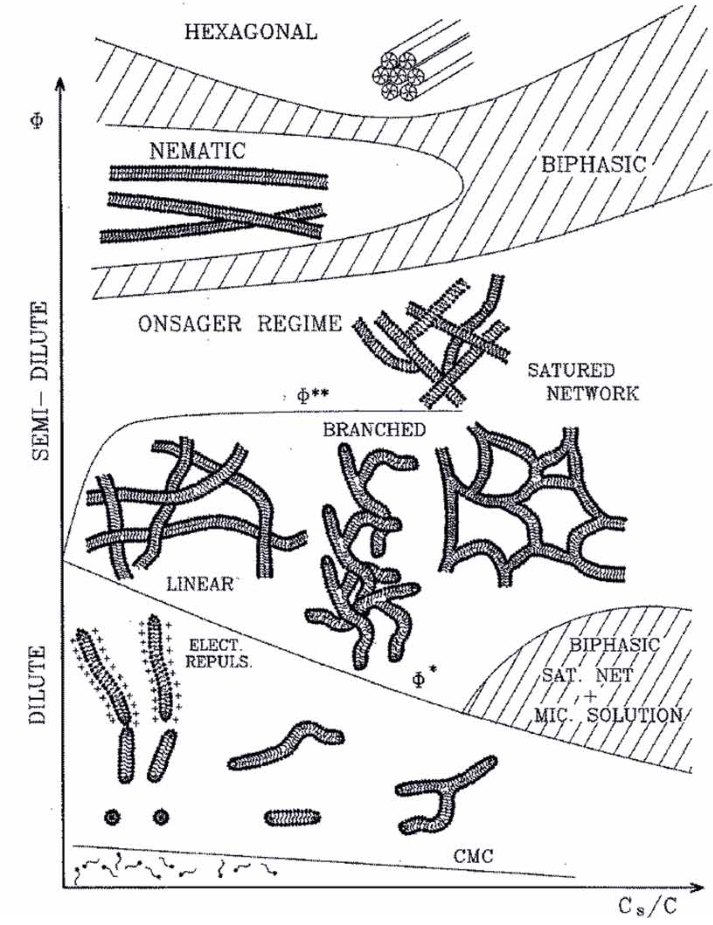
\includegraphics[width=0.5\textwidth]{imagens/artigos/estruturas_regimes_concentracoes_cates_fielding}
			%\caption[Diagrama de fase esquemático para estruturas alongadas]{Diagrama de fase esquemático mostrando as diferentes estruturas alongadas que podem ser formadas em sistemas com surfactantes e sais. Em especial, vale destacar a concentração micelar crítica, \cmc, e a concentração de sobreposição, \(\phi^*\), que será introduzida posteriormente no texto. Além disso, o sistema com micelas gigantes pode tanto possuir micelas lineares, ramificadas, e formando redes. Adaptado de \citeauthor{Herb1994}}
			\caption{Diagrama de fase esquemático mostrando as diferentes estruturas alongadas que podem ser formadas em sistemas com surfactantes e sais. Em especial, vale destacar a concentração micelar crítica, \cmc, e a concentração de sobreposição, \(\phi^*\), que será introduzida posteriormente no texto. Além disso, o sistema com micelas gigantes pode tanto possuir micelas lineares, ramificadas, e formando redes. Adaptado de \citeauthor{Herb1994}}
			\label{fig:regimes_e_estruturas_lequeux}
		\end{figure}
	\index{micelas gigantes!regime semidiluído}
	\index{micelas gigantes!\cwlm}
	\index{micelas gigantes!\cmc}
	\index{micelas gigantes!ramificações}
	\index{micelas gigantes!rede}
		
		As micelas gigantes possuem alguns comprimentos característicos. Começando do maior, temos o comprimento de contorno, \(L_c\), que vai de uma ponta à outra da micela. Em solução, as micelas geralmente estão enoveladas, dependendo de sua rigidez, e o tamanho desse novelo é conhecido como raio de giro, \(R_g\).  Por sua vez, a rigidez intrínseca, cujo tamanho é definido pelo comprimento de persistência \(l_p\), também está relacionada ao comprimento de Kuhn, \(k_L\) pela relação \(k_L=2l_p\).\cite{Dreiss2007} A proporção entre o comprimento de contorno e de persistência de uma micela informa o quão flexível essa micela é. Por exemplo, micelas longas e com comprimento de persistência curto são bastante flexíveis, porém micelas curtas, da mesma ordem do comprimento de contorno, se comportam como cilindros rígidos. O menor dos comprimentos é o raio da seção transversal (\(r_{\mathrm{CS}}\)), da ordem do raio de micelas esféricas, em torno de poucos nanômetros. O raio de seção transversal das micelas é próximo ao comprimento da cadeia do surfactante, que está em torno de 2 nm. O comprimento de persistência varia de 15 a 1000 nm, e o comprimento de contorno varia de 4 a 3600 nm.\cite{Dreiss2007} A \autoref{fig:escalas_tamanho_mg} mostra as escalas de tamanho das micelas gigantes.
		\index{micelas gigantes!comprimento de persistência \(l_p\)} 
		\index{micelas gigantes!comprimento de contorno \(L_c\)} 
		\index{micelas gigantes!raio de giro \(R_g\)} 
		\index{micelas gigantes!comprimento de Kuhn \(k_L\)} 
		\index{micelas gigantes!raio de seção transversal \(r_\mathrm{CS}\)}
		\index{micelas gigantes!tamanho da rede \(\xi\)}
		\index{micelas gigantes!comprimento entre dois pontos de entrelaçamento \(l_e\)}
		
		\begin{figure}[h]
			\centering
			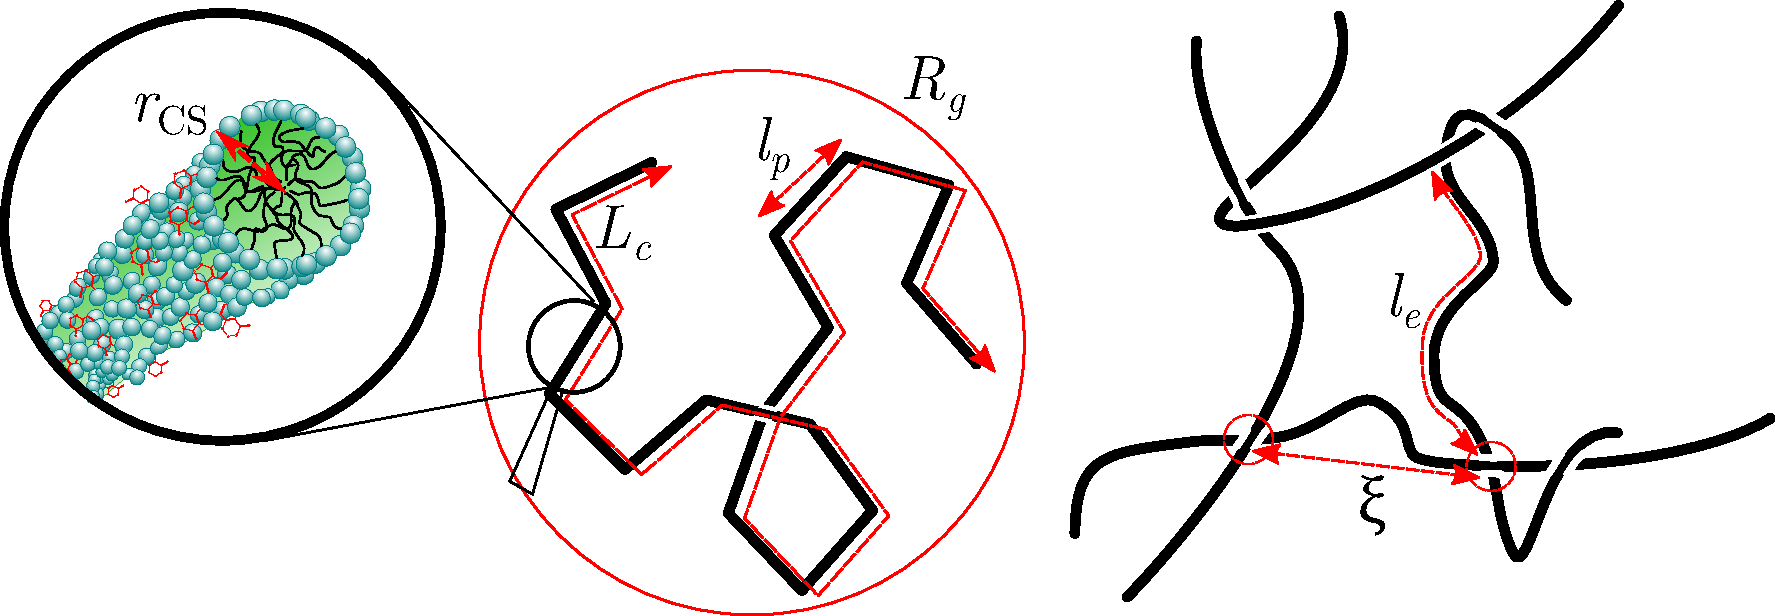
\includegraphics[width=\textwidth]{imagens/artigos/escalas_tamanho_MG}
			%\caption[Escalas de tamanho de micelas gigantes]{Escalas de tamanho de micelas gigantes. Da esquerda para a direita, temos o raio de seção transversal \(r_\mathrm{CS}\), o comprimento de contorno \(L_c\), o comprimento de persistência \(l_p\), o raio de giro \(R_g\), o tamanho da rede polimérica \(\xi\) e o comprimento entre dois pontos de entrelaçamento \(l_e\). Esses dois parâmetros serão introduzidos na \autoref{sec:teo_reologia_oscilatoria}. Imagem adaptada de \citeauthor{Dreiss2007} e \citeauthor{Hoffmann1992a}}
			\caption{Escalas de tamanho de micelas gigantes. Da esquerda para a direita, temos o raio de seção transversal \(r_\mathrm{CS}\), o comprimento de contorno \(L_c\), o comprimento de persistência \(l_p\), o raio de giro \(R_g\), o tamanho da rede polimérica \(\xi\) e o comprimento entre dois pontos de entrelaçamento \(l_e\). Esses dois parâmetros serão introduzidos na \autoref{sec:teo_reologia_oscilatoria}. Imagem adaptada de \citeauthor{Dreiss2007} e \citeauthor{Hoffmann1992a}}
			\label{fig:escalas_tamanho_mg}
		\end{figure}
		
		Por possuírem tamanhos finitos, as micelas gigantes apresentam pontas. O empacotamento moleculas nas pontas é diferente do corpo cilíndrico, caso contrário, não possuiriam a curvatura necessária para ``fechar'' um cilindro. Por esse motivo, as pontas possuem uma energia maior que na parte cilíndrica da micela.\cite{May2001a} Se a causa principal para a mudança no parâmetro de empacotamento for a presença de sais como NaSal, segue que a concentração de NaSal incorporado às pontas deve ser diferente do corpo micelar. O empacotamento diferenciado das pontas pode ser facilmente observado em micelas mais espessas, como de copolímeros em bloco (\autoref{fig:pontas_inchadas_danino2009}). \index{micelas gigantes!pontas}
		
		\begin{figure}[h]
			\centering
			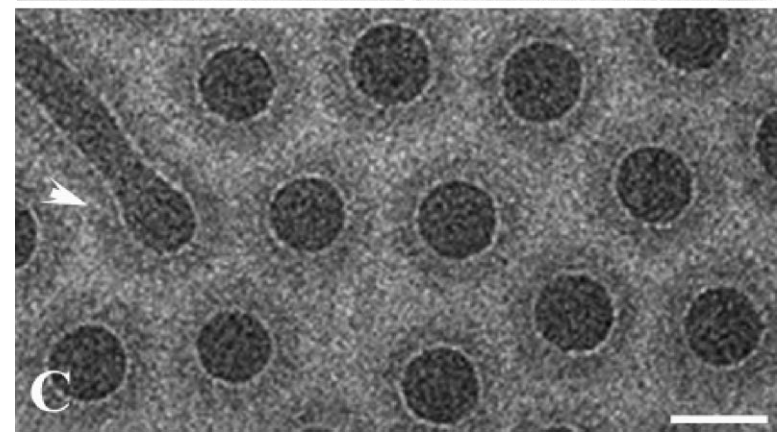
\includegraphics[width=0.5\textwidth]{imagens/artigos/Cryo_TEM_Pontas_Danino_2009}
			\caption{Imagens de microscopia de transmissão a temperaturas criogênicas (Cryo-TEM) e uma solução de copolímero em dibloco neutro P3017-BdEO na concentração de 10 mg.mL\menosUm{} em tampão de fosfato. Nessa mistura, há a coexistência de micelas esféricas e de micelas alongadas curtas. É possível observar o interior da micela, mais escuro, e a coroa, mais clara, indicada pela seta branca. Além disso, a ponta inchada se mostra muito evidente. A barra de escala é igual a 50 nm. Retirado com permissão de \citeauthor{Shimoni2009}}
			\label{fig:pontas_inchadas_danino2009}
		\end{figure} \index{micelas gigantes!Cryo-TEM}
				
		Caso mais moléculas de surfactante se dirijam à parte cilíndrica micelar, haverá a formação de micelas mais compridas, caso contrário, haverá um número maior de micelas mais curtas. Assim, quanto maior for a energia das pontas, maior será o comprimento da micela.\cite{May2001a}
		
		Acima da concentração de sobreposição \(\phi^*\), é possível calcular, pela teoria do campo médio, o comprimento de contorno médio \(\overline{L_c}\), relacionando-o à energia das pontas, \(E_c\) (\autoref{eqn:l_contorno_neutra})\cite{Cates1990}. Essa teoria considera que o comprimento de persistência é muito maior que o raio de seção transversal, e que o volume excluído pelas cadeias pode ser considerado pelo sistema completo, ao invés de ser tratado localmente.
		\index{micelas gigantes!concentração de sobreposição} \index{micelas gigantes!energia das pontas}
		
		\begin{equation}
			\overline{L_c} \approx \phi^{\frac{1}{2}} \exp \left(\dfrac{E_c}{2k_BT}\right)
			\label{eqn:l_contorno_neutra}
		\end{equation} % ref Cates
		
		\noindent onde \(\phi\) é a fração volumétrica de surfactante. 
		
		Porém, a contribuição eletrostática não foi considerada. A carga na superfície micelar tende a quebrar as micelas. Isso resulta numa diminuição de sua flexibilidade, e também do comprimento total das micelas, pois a energia das pontas é contrabalanceada pela energia dessa repulsão eletrostática, denominada \(E_e\). O comprimento de contorno médio ajustado é dado por \cite{Magid2000b, Mackintosh1990}
		\index{micelas gigantes!efeito da eletrostática}
		\index{micelas gigantes!energia de repulsão eletrostática}
		
		\begin{equation}
			\overline{L_c} \approx \phi^{\frac{1}{2}} \exp \left(\dfrac{E_c - E_e}{2k_BT}\right)
			\label{eqn:l_contorno_carregada}
		\end{equation}

		A concentração de transição na presença de efeitos eletrostáticos é dada pela \autoref{eqn:conc_overlap_por_Ec}\cite{Magid2000b, Mackintosh1990}, que é dependente do comprimento de Bjerrum \(\lambda_B\), descrito na \autoref{sec:coloides_atracao_coloidal}.
		
 		\begin{equation}
			\phi^* = \left( \frac{k_B T \lambda_B r_{\mathrm{CS}} \nu^{*2}}{E_c} \right) ^ 2
			\label{eqn:conc_overlap_por_Ec}
		\end{equation} 
	
		\noindent onde \(\nu^{*2}\) é a carga efetiva por unidade de comprimento micelar.
		 
		O número de agregação característico \(\overline{N}\) é dado por \cite{Mackintosh1990}
		
		\begin{equation}
			\overline{N} = 2 \phi ^{\frac{1}{2}} \exp \left[ \frac{1}{2} \left( E_c - E_e \right) \right]
			\label{eqn:distrib_tamanhos_micelas}
		\end{equation} 
		\index{micelas gigantes!número de agregação característico}
		 
		Porém, essas equações não consideram a formação de \emph{loops} ou de pontos de ramificação. A formação de \emph{loops} elimina a energia das pontas, em troca de perda de entropia conformacional. Pontos de ramificação, assim como as pontas de micelas, possuem um empacotamento diferente do corpo micelar, mas com a curvatura oposta.
		\index{micelas gigantes!loops}
		
		A reologia de sistemas onde se formam redes difere fortemente de quando as cadeias estão lineares.\cite{Cates2006, Lequeux1992a} Uma característica importante dos pontos de ramificação é que eles são lábeis, isto é, podem se mover pela cadeia. Nesse caso, o comprimento de contorno \(\overline{L_c}\) não possui o mesmo significado físico. Nesse caso, \(\overline{L_c}\) denota distância até a cadeia mais próxima, ou o ponto de junção na rede. Isso ocorre porque o sistema ramificado, em escalas de tamanho maiores que \(\overline{L_c}\), oferece uma reserva para o comprimento de contorno, que pode ser armazenado, ou emprestado, para outras cadeias da rede. \cite{Cates2006} 
		
		\section{Comportamento reológico}
		
		\subsection{Reologia oscilatória} \index{micelas gigantes!reologia oscilatória}
		\label{sec:teo_reologia_oscilatoria}
		Caso o comprimento das micelas seja longo o suficiente, isto é, a energia das pontas for grande, as soluções micelares começam a apresentar características elásticas. Isso é facilmente observado pelo fenômeno chamado de \emph{recoil}, quando uma solução é agitada numa direção, e se observa que o fluxo inverte de sentido após algum tempo, evidência de viscoelasticidade.\cite{Hoffmann1988a}
		
		Quando a concentração é aumentada significativamente, e ultrapassa \(\phi^*\), e as micelas começam a se sobrepor e a entrelaçar.\cite{Cates1990} A separação das cadeias é conhecido como o tamanho da rede (\emph{mesh size}), \(\xi\). Caso a concentração e o comprimento das micelas aumente, as soluções podem se tornar bastante rígidas, semelhantes a géis. 
		\index{micelas gigantes!tamanho da rede \(\xi\)}

		Quando essa rede de micelas é submetida a uma tensão, processos de relaxação começam a ocorrer no material. Micelas gigantes possuem, essencialmente, dois processos de relaxação de tensão, a reptação, presente também em polímeros, e a quebra e recombinação, oriunda de sua natureza autoassociativa.\cite{Cates1990} Nos modelos mais simples, o decaimento da tensão (\(\mu(t)\)) é exponencial, com um tempo de decaimento característico (\(\tau_{\mathrm{rel}}\)), que é modulado por \(G\). Essas relações estão expostas nas equações \ref{eqn:decaimento_stress}\cite{Cates1990} e \ref{eqn:decaimento_G_t}\cite{Cates2006}. Essas equações, e grande parte da teoria sobre o relaxamento de micelas gigantes, foram propostas em uma série de artigos \cite{Cates1987, Cates1990}
		
		\index{micelas gigantes!mecanismos de relaxação} 
		\index{micelas gigantes!reptação}
		\index{micelas gigantes!quebra e recombinação}
		\index{micelas gigantes!modelo de Cates}
		
		\begin{equation}
			\mu(t)  \approx \exp \left(  \frac{-t}{\tau_{\mathrm{rel}}} \right)
			\label{eqn:decaimento_stress}
		\end{equation} % ref Berret 1993
		
		\begin{equation}
			G(t) \equiv G \mu(t)	
			\label{eqn:decaimento_G_t}
		\end{equation} % ref Cates 1990
		\index{micelas gigantes!relaxação da tensão}
		
		A reptação é o movimento da cadeia através de um tubo formado pelos pontos de contato com as cadeias vizinhas, que oferecem obstáculos para o movimento. O modelo considera uma cadeia primitiva no centro do tubo formado pela média das várias conformações possíveis de uma cadeia real. \cite{Goodwin2008} Quando a micela alongada sai do tubo inicial, por movimentos em ambos os sentidos, seu processo de reptação terminou. O termo reptação foi proposto por Pierre de Gennes\cite{DeGennes1971, Gennes1983}, 
		que posteriormente ganhou o prêmio Nobel em 1991\cite{DeGennesNobel}, e faz menção ao movimento de rastejar de répteis (do latim \emph{reptare}). \cite{Goodwin2008}
		\index{micelas gigantes!reptação}

		\begin{figure}[h]
			\centering
			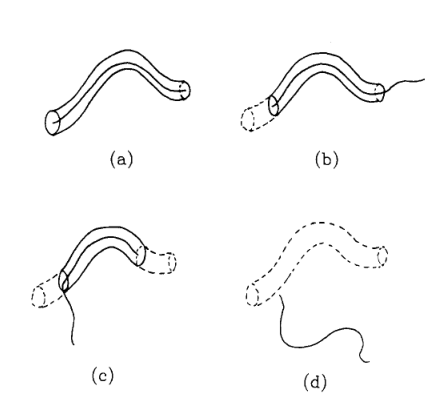
\includegraphics[width=0.5\textwidth]{imagens/artigos/reptacao_cates_1987}
			\caption{Reptação de uma cadeia primitiva pelo tubo formado pelos pontos de contato com as cadeias vizinhas. (a) Em \(t=0\), o tubo é definido. (b, c) A difusão da cadeia ocorre pelas extremidades do tubo, devido às barreiras de entrelaçamento. (d) Após um \(t \ge \tau_\mathrm{rep}\), nada do tubo original permanece, e o novo tubo não tem tensão acumulada. Imagem retirada de \citeauthor{Cates1987}}
			\label{fig:reptacao_cates1987}
		\end{figure}
		
		O tempo de reptação é, claramente, dependente do comprimento da cadeia, e pode ser estimado por\cite{Cates1990}
		
		\begin{equation}
			\tau_\mathrm{rep} \simeq \frac{\overline{L_c}^2}{D_c}
			\label{eqn:tau_rep_comprimento_contorno}
		\end{equation} % ref Cates 1990
		
		\noindent onde \(D_c\) é a constante de difusão curvilinear da cadeia dentro do tubo.
		
		Já o tempo que a micela demora para quebrar é dependente de seu comprimento e de uma constante de velocidade dessa ``reação'', \(k_\mathrm{quebra}\).\cite{Cates1990} A teoria do campo médio assume que é improvável que essa recombinação ocorra entre as mesmas cadeias que se quebraram. Além disso, é estimado que o tempo para a recombinação é o mesmo que para a quebra. 
		
		\begin{equation}
			\tau_{\mathrm{quebra}} = \left(k_\mathrm{quebra}\overline{L_c}\right)^{-1}
			\label{eqn:tempo_quebra_comp_contorno}
		\end{equation} % ref Cates 1990
		\index{micelas gigantes!quebra e recombinação}
		
		Por último, o módulo no platô \(G\) (também conhecido, dependendo da referência, como \(G_0\))  é dependente da quantidade de pontos de contato das micelas, que, por sua vez, é dependente da fração volumétrica de surfactante \(\phi\).\cite{Cates1990} \index{micelas gigantes!módulo no platô \(G\)}
		
		\begin{equation}
			G \sim \phi^{2{,}3}  
			\label{eqn:scaling_g0}
		\end{equation} % ref Cates 1990
		
		Dois tempos de relaxação com magnitudes semelhantes resultaria em um decaimento diferente do monoexponencial. Porém, se a magnitude do tempo de quebra e recombinação for muito menor (mais rápido) do que o tempo de reptação, \( \tau_{\mathrm{quebra}} \ll \tau_\mathrm{rep} \), o tempo de relaxação total se reduz à média geométrica dos dois tempos (\autoref{eqn:tau_rel_dois_taus}). Quando uma solução de micelas gigantes segue essa consideração, o modelo de Maxwell também pode ser aplicado para descrever seu comportamento reológico.\cite{Berret1993a}
		
		\begin{equation}
			\tau_{\mathrm{rel}} \simeq \left( \tau_\mathrm{rep} \tau_\mathrm{quebra} \right) ^ \frac{1}{2}
			\label{eqn:tau_rel_dois_taus}
		\end{equation} \index{micelas gigantes!tempo de relaxação médio}
		
		Neste trabalho, serão apresentados regimes que tanto seguem quanto não seguem essa consideração. Há duas maneiras de se determinar isso. Uma é pelo ajuste do modelo de Maxwell (\autoref{sec:modelo_maxwell}). Quanto melhor for o ajuste, mais correta é a consideração da \autoref{eqn:tau_rel_dois_taus}. Outra maneira é pelos gráficos de Cole-Cole (\autoref{fig:colecole_berret}), onde G'' é plotado em função de G'. Caso haja somente um tempo de relaxação, e um decaimento exponencial, será observado um semicírculo perfeito, de acordo com a \autoref{eqn:cole_cole}. Esse tipo de gráfico por ser normalizado por \(G\), reduzindo a escala dos valores dos eixos e facilitando a comparação entre curvas diferentes.\cite{Berret1993a}
		
		\begin{equation}
			\left(G' - \frac{G}{2}\right)^2 + G''^2 = \frac{G^2}{4}
			\label{eqn:cole_cole}
		\end{equation} \index{micelas gigantes!Cole-Cole}
		
		\begin{figure}[h]
			\centering
			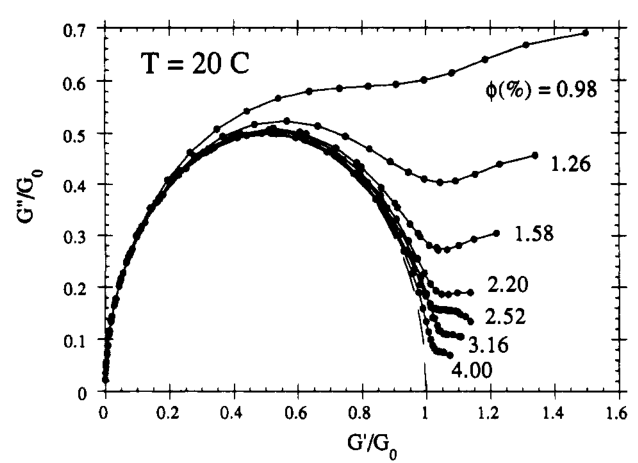
\includegraphics[width=0.5\textwidth]{imagens/artigos/ColeCole_Berret_Appel_Porte_1993}
			\caption{Diagrama de Cole-Cole para cloreto de cetilpiridínio (C\textsubscript{16}PyCl) e salicilato de sódio diluídas em soluções de cloreto de sódio 500 \mM. A proporção \Sal:C\textsubscript{16}PyCl foi mantida constante em 0,5. A fração mássica de surfactante foi de 0,98\% a 4\%. O semicírculo indica o comportamento Maxwelliano ideal, com um único tempo de relaxação. Imagem retirada de \citeauthor{Berret1993a}}
			\label{fig:colecole_berret}
		\end{figure}

		\index{micelas gigantes!Rouse} \index{micelas gigantes!breathing modes@\textsl{breathing modes}}
		
		Diagramas de Cole-Cole ajudam a identificar a região onde outros mecanismos de relaxação começam a operar. Um desses modos é chamado de ``respiração'' das cadeias (\emph{breathing motions}), onde ocorrem flutuações no comprimento do tubo, ao invés da reptação completa das cadeias. Além disso, pode ocorrer a movimentação de Rouse, já descrita previamente para a área de polímeros. \cite{Granek1992}
		A região onde esses modos começam a se tornar relevantes é observada no final do diagrama de Cole-Cole, quando, ao invés de permanecer no semicírculo, a curva começa a subir. No reograma (G' e G'' por \(\omega\)), isto é observado quando G'' atinge um valor mínimo e começa a subir, sendo que o modelo de Maxwell prevê somente sua queda.
		
		Nesse ponto, a diferença nos valores entre o módulo no platô e o ponto onde G'' começa a subir é proporcional ao comprimento da cadeia entre dois pontos de entrelaçamento e ao comprimento das micelas, \cite{Berret1993a} 
		\index{micelas gigantes!comprimento entre dois pontos de entrelaçamento \(l_e\)}
		
		\begin{equation}
			\frac{G''_\mathrm{min}}{G'_\infty} \sim \frac{l_e}{\overline{L_c}}
			\label{eqn:mesh_contorno_por_reologia}
		\end{equation} % ref Berret 1993

		\noindent onde \(G'_\infty\) é o módulo no platô extrapolado para a frequência onde ocorre o mínimo de G''.
		
		O valor de \(l_e\) é proporcional ao tamanho da rede polimérica \(\xi\) e ao comprimento de persistência, \cite{Berret1993a}
		
		\begin{equation}
			l_e \sim \xi^{\sfrac{5}{3}} l_p^{\sfrac{-2}{3}}
			\label{eqn:mesh_comprimento_entrelacamento}
		\end{equation} % ref Berret 1993
		
		E por sua vez, o tamanho da rede é dependente de \(G'_\infty\), que é igual a \(G\), que, por sua vez, é dependente de \(\phi\), \cite{Berret1993a}
		
		\begin{equation}
			\xi \sim \left(  \frac{k_BT}{G'_\infty} \right) ^ \frac{1}{3}
		\end{equation} % ref Berret 1993
		\index{micelas gigantes!módulo no platô \(G\)}
		
		Alguns autores reportam ser possível obter o tempo de relaxação pelo inverso da frequência onde \(G''_\textrm{min}\),
		
		\begin{equation}
			\dfrac{1}{\tau_{\mathrm{quebra}}} \approx \omega_{\textrm{min}}
			\label{eqn:tauquebra_g2min}
		\end{equation}
		
		\noindent porém, essa estimativa não é estritamente correta e não possui base física.\cite{CalabreseTese}
	
		O reograma para soluções de micelas gigantes que seguem o modelo de Maxwell é bastante similar ao apresentado na página \pageref{fig:modelo_maxwell}. Neste trabalho, várias soluções seguiram esse modelo, como será visto na \autoref{sec:reologia_oscilatoria_experimental_agua}.
		
		Esse comportamento pode ser interpretado como apresentado a seguir. Em baixas frequências de perturbação (longos tempos), as micelas possuem tempo suficiente para deslizar umas pelas outras, então a maior parte da energia fornecida é perdida, logo o módulo viscoso, ou de perda, possui valores altos. Em frequências altas, a rede micelar e os entrelaçamentos conseguem armazenar a energia, não possuindo tempo suficiente para deslizar, então o módulo elástico, ou de armazenamento, é alto. Na região intermediária, ambos os mecanismos estão presentes, parte da energia é perdida e parte é armazenada, sendo que no ponto de cruzamento, exatamente metade da energia é preservada e metade é perdida.
		
		\section{Curvas de fluxo e a dependência da concentração de sal na viscosidade no repouso} \index{micelas gigantes!curvas de fluxo} \index{micelas gigantes!perfil de viscosidade} \index{micelas gigantes!NaSal} \index{micelas gigantes!\CTAB}
			
		Surfactantes catiônicos, como os haletos de alquiltrimetilamônio ou alquilpiridínio são frequentemente utilizados para a formação de micelas gigantes utilizando sais orgânicos, como o salicilato de sódio, porém vários outros sais conseguem induzir o crescimento micelar. Esse tipo de sistema foi bastante estudado por Hoffmann, para uma variedade de sais e surfactantes\cite{Rehage1991, Rehage1988, Hoffmann1992a} e também por outros autores.\cite{Wei2013, Hartmann1998, Lutz-Bueno2016a,Lutz-Bueno2017, Cappelaere1998, Pleines2019, Clinckspoor2015, Raghavan2002a, Davies2006}
		
		Tais sais orgânicos possuem uma região hidrofóbica que consegue se inserir na superfície micelar, e ao mesmo tempo manter o grupo carregado exposto à água, na superfície. Isso diminui a carga superficial micelar, aumentando o parâmetro de empacotamento e induzindo o crescimento das micelas. Sais inorgânicos, como Cl\textsuperscript{-}, também podem promover o crescimento, mas necessitam de concentrações uma ordem de grandeza maiores. Por exemplo, é necessária a concentração de aproximadamente 4 mol.L\menosUm{} de NaCl para gerar micelas com efeitos viscosos semelhantes aos gerados por NaSal, numa solução com \CTAB 100{} \mM.\footnote{Dados não publicados}
		
%		\begin{figure}[h]
%			\centering
%			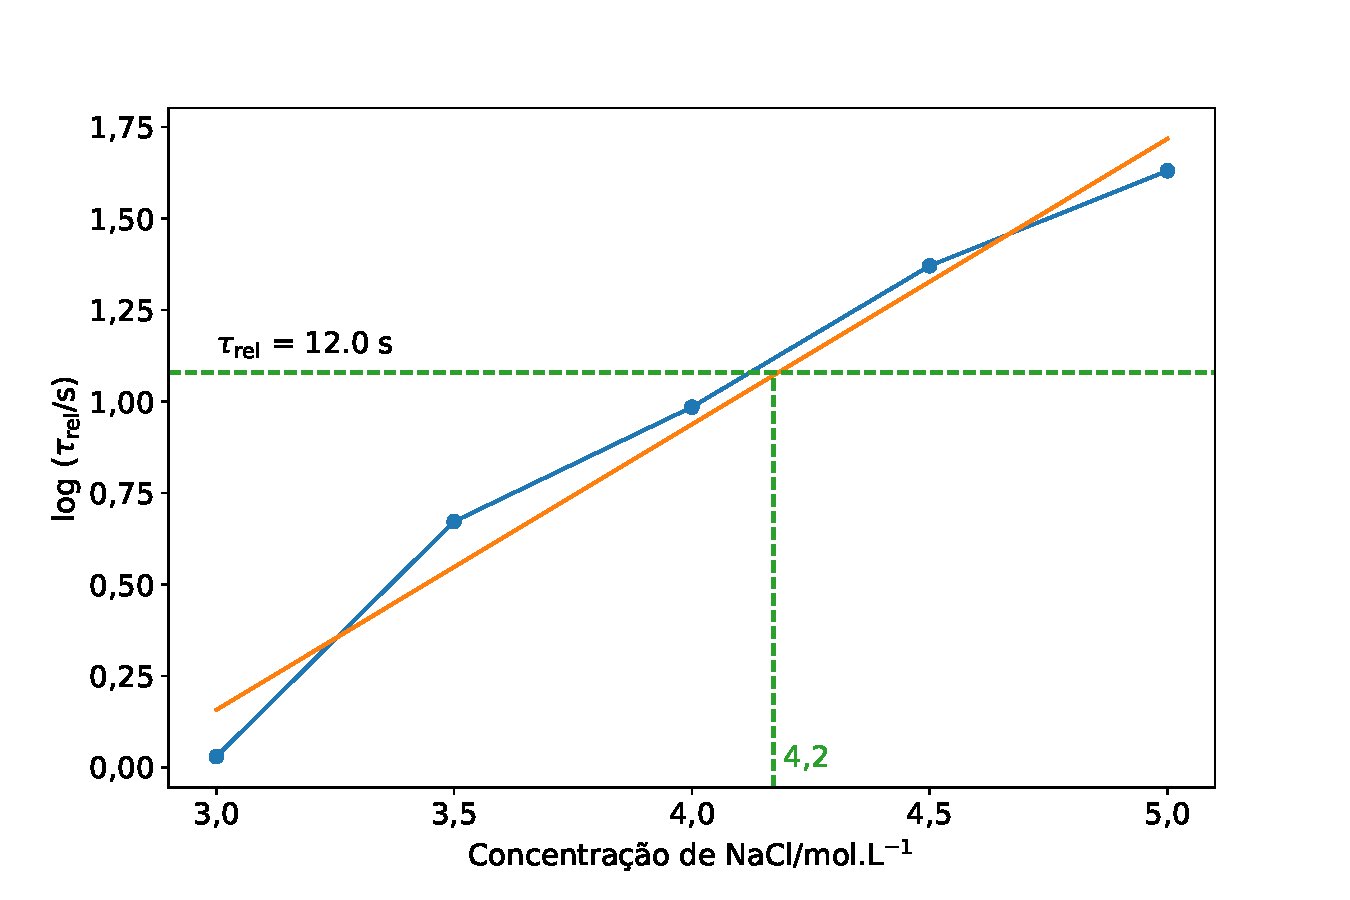
\includegraphics[width=0.7\textwidth]{imagens/reologia/equivalencia_nasal_nacl}
%			\caption{Tempos de relaxação para amostras de \CTAB{} 100 \mM{} e concentrações crescentes de NaSal. A linha reta simboliza o ajuste. O tempo de relaxação dessa solução  }
%			\label{fig:equivalencia_nasal_nacl}
%		\end{figure}
		
		
		\index{micelas gigantes!OHCA}
		A viscosidade das soluções de surfactantes catiônicos e sais orgânicos é dependente da concentração e da afinidade do sal pela micela que, por sua vez, depende de sua estrutura. Além disso, a afinidade do sal altera o perfil de viscosidade. Sais com pouca afinidade, como ortometilbenzoato de sódio, possuem um único máximo de viscosidade, já sais como o salicilato de sódio e o orto-hidroxicinamato de sódio geram perfis com dois máximos de viscosidade.\cite{Clinckspoor2015, Ito2014c}
		A quantidade de salicilato que se concentra na superfície micelar é alta, cerca de 93\%, muito mais do que os íons Cl\textsuperscript{-} e Br\textsuperscript{-}.\cite{Rehage1991}
		
		Tais soluções de surfactante e sal aromático podem ser estudadas tanto por reologia oscilatória quanto por curvas de fluxo. Soluções de micelas gigantes, quando submetidas à uma taxa de cisalhamento crescente, começam a se alinhar ao fluxo, diminuindo a viscosidade aparente da solução. Isso as caracteriza como fluidos pseudoplásticos. Quando a taxa de cisalhamento é baixa, a viscosidade não se altera, e pode-se obter uma grandeza conhecida como viscosidade no repouso \(\eta_0\) por uma variedade de técnicas (\autoref{sec:teoria_fluidos_NN}). \index{micelas gigantes!alinhamento ao fluxo}
		
		As alterações no perfil de viscosidade são devidas à mudanças nos mecanismos de relaxação das micelas, que por sua vez são dependentes da estrutura das micelas em solução, de sua carga e sua concentração. O perfil para \CTAB{} e NaSal, disposto na \autoref{fig:regioes_rh}, é geralmente dividido em cinco regiões.\cite{Rehage1988}
		
		\begin{enumerate} \index{micelas gigantes!perfil de viscosidade|textbf}
			\item[I] Região altamente diluída, onde há micelas esféricas, seguido de micelas cilíndricas curtas e, em concentrações um pouco mais altas, de micelas gigantes muito distantes umas das outras.
			\item[II] Região onde ocorre aumento no número de micelas e crescimento das mesmas, levando ao entrelaçamento e aumento rápido da viscosidade. As micelas estão positivamente carregadas, e lineares. O mecanismo principal de relaxação nesta região é a reptação, porém as soluções não seguem o modelo de Maxwell perfeitamente, pois há um espectro de processos de relaxação. \cite{Rehage1988}
			 O valor de \(G\) dessa região é menor do que nas próximas. \cite{Rehage1991}
			\item[III] Região onde a carga das micelas continua a diminuir com a incorporação crescente de NaSal, levando à uma diminuição da carga superficial. Ao invés de micelas lineares, ocorre a formação de uma rede ramificada de micelas, e a solução começa a seguir o modelo de Maxwell. Quando a solução se aproxima da equimolaridade, a carga superficial das micelas se aproxima a 0. Nessa região, o processo de relaxação principal é a quebra e recombinação.
			\item[IV] Região onde a carga das micelas começa a ficar mais negativa devido ao excesso de salicilato em solução\cite{Olsson1986a}, mas alguns trabalhos discordam, citando que o salicilato extra pode se encontrar fora, como um contraíon.\cite{Cassidy1996} A estrutura das micelas ainda é ramificada. % todo: colocar uma ref disso. Rehage?
			A carga superficial pode levar a uma diminuição na taxa de colisão entre as micelas e no aumento do comprimento de persistência, aumentando o tempo de relaxação estrutural. A viscosidade menor nesta região, em relação à região II, pode se dever aos íons \Sal{} livres, que ajudam nos mecanismos de dissipação de tensão.\cite{Shikata1988} 
			\item[V] Região onde a quantidade de salicilato aumentou em demasia, e, ao invés do crescimento micelar ocorrer, existe somente a transição para micelas cilíndricas curtas, ou esféricas, com grande excesso de salicilato.
		\end{enumerate}
		
		\begin{figure}[h]
			\centering
			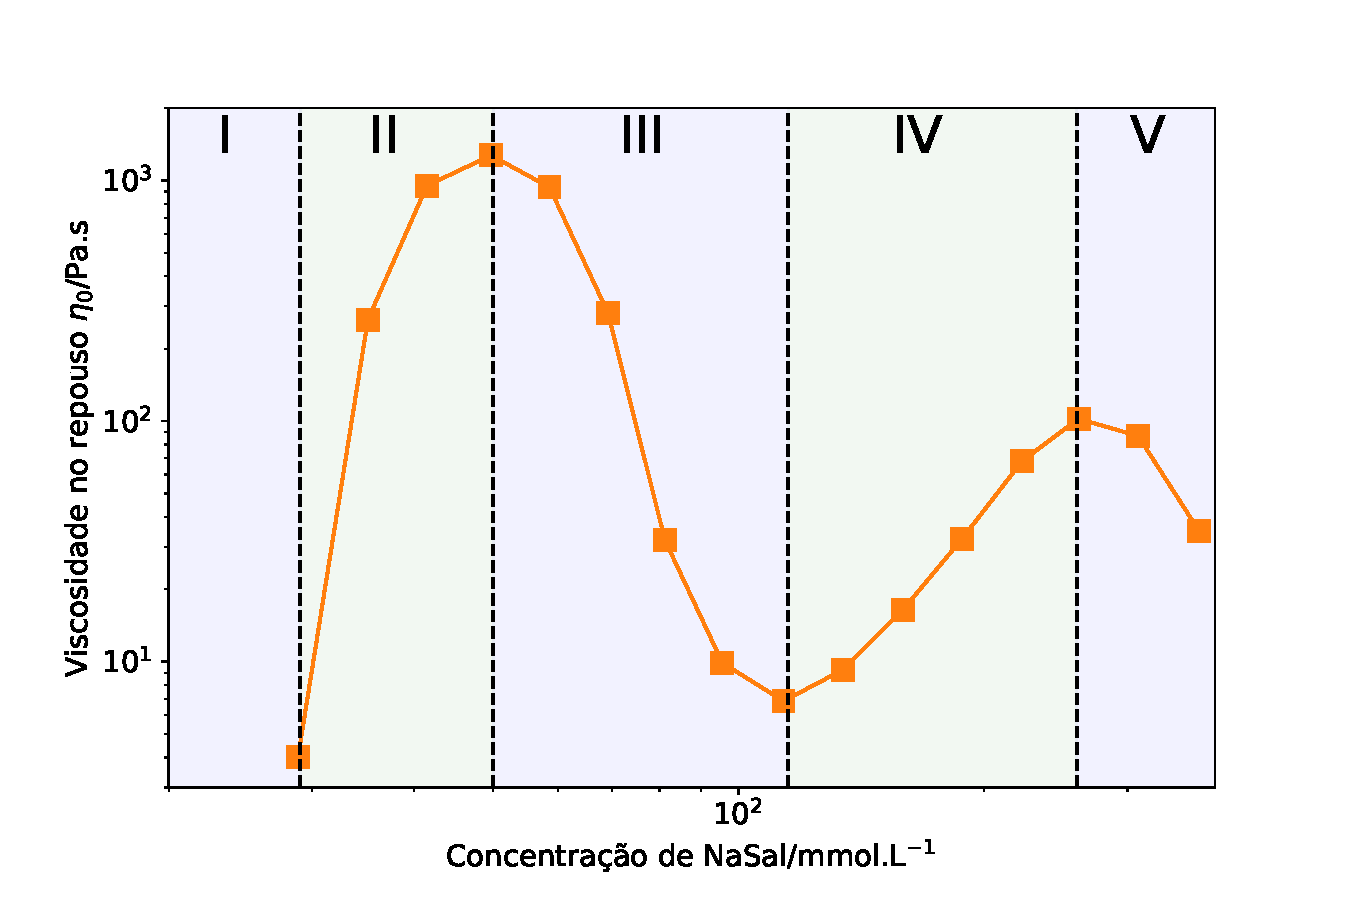
\includegraphics[width=0.7\textwidth]{imagens/reologia/regioes_RH}
			\caption{Perfil de viscosidade de soluções com \CTAB{} 100 \mM{} e concentrações crescentes de NaSal. As linhas verticais separam as cinco regiões, onde o comportamento e a estrutura micelar são diferentes. Este diagrama foi obtido neste trabalho, e as regiões foram delimitadas de acordo com \citeauthor{Rehage1988}.}
			\label{fig:regioes_rh}
		\end{figure}

		Além desses fatores relativos ao salicilato, há uma contribuição do surfactante. A viscosidade do sistema \CTAB{} e NaSal é maior, em todas as proporções, que a viscosidade do sistema cloreto de hexadecilpiridínio (C\textsubscript{16}PyCl) e NaSal \cite{Lutz-Bueno2017}
		Essa diferença ocorre, de acordo com Hoffmann,\cite{Hoffmann2010, Hoffmann2012a, Yamashita2006} devido aos contatos ``grudentos'' (\emph{sticky contacts}) causados pela atração entre grupos metila do \CTAB, hidrofóbicos, com os outros grupos metila de micelas vizinhas. Isso aumenta o tempo de relaxação estrutural, pois o deslizamento entre as micelas se torna mais lento, levando à maior viscosidade. O mesmo mecanismo não pode ocorrer, pois o grupo piridínio não possui tais metilas. \index{micelas gigantes!sticky contacts@\textsl{sticky contacts}} 
		

		\section{Termodinâmica de micelas} \index{micelas gigantes!termodinâmica}
		
		Numa solução acima da concentração micelar crítica, existem tanto moléculas de surfactante livres quanto moléculas de surfactante nos agregados. Necessariamente, essas moléculas devem possuir, todas, o mesmo potencial químico \(\mu\), \cite{Israelachvili2011}
		
		\begin{equation}
			\mu = \mu_N = \mu_N^\circ + \dfrac{k_B T}{N} \log \left( \dfrac{X_N}{N} \right) = \mathrm{constante}
			\label{eqn:potencial_quimico_micelas}
		\end{equation} \index{micelas gigantes!potencial químico}
		
		\noindent onde \(\mu_N\) é o potencial químico médio de uma molécula num agregado com número de agregação N, \(\mu_N^\circ\) é o potencial químico padrão médio para uma molécula no agregado com número de agregação N, \(X_N\) é a concentração (ou atividade) de moléculas em agregados com o determinado \(N\). A energia por agregado é \(N\mu_N^\circ\).\cite{Israelachvili2011} \(X_N\) pode ser descrito como fração volumétrica ou molar, dependendo das unidades de \(\mu\) utilizadas.\cite{Israelachvili2011}
		
		Logo, no equilíbrio, temos que, para agregados com \(N=1, 2, 3, \dots\):
		
		\begin{equation}
			\mu = \mu_1^\circ + k_B T \log X_1 = \mu_2^\circ + \dfrac{1}{2} k_B T \log \dfrac{X_2}{2} = \mu_3^\circ + \dfrac{1}{3} k_B T \log \dfrac{X_3}{3} = \cdots
		\end{equation}
		
%		Para a agregação, é necessário que a energia coesiva entre as moléculas no agregado seja maior do que no estado disperso. É necessário que \(\mu_N^\circ\) seja menor que \(\mu_1^\circ\) para algum valor, ou conjunto de valores, de \(N\). Para micelas cilíndricas, a energia de um agregado pode ser aproximada assumindo uma energia de ``ligação'' entre os monômeros, \(-\alpha k_B T\), onde \(\alpha\) é uma constante positiva dependente da força das interações intermoleculares.
%		
%		\begin{equation}
%			N \mu_N^\circ = -(N - 1) \alpha k_B T
%			\label{eqn:potencial_quim_cilindro1}
%		\end{equation}
%		
%		O potencial químico do agregado \(\mu_N^\circ\) é então dado por
%		
%		\begin{equation}
%			\mu_N^\circ = \mu_\infty^\circ + \alpha k_B T / N
%			\label{eqn:potencial_quim_cilindro2}
%		\end{equation}
%		
%		\noindent onde \(\mu_\infty^\circ\) é o potencial químico numa molécula com um número infinito de agregação.
	
		De forma geral, o potencial químico dos agregados aumenta com o número de agregação. Deve-se considerar a diferença no potencial químico dessas duas espécies, para entender em qual concentração ocorre a transição entre monômeros e agregados, a \cmc, \cite{Israelachvili2011}
		
		\begin{equation}
			X_N = N \left[ X_1 \exp \left(\dfrac{\mu_1^\circ - \mu_N^\circ}{k_B T}\right) \right] ^ N
			\label{eqn:termodinamica_diferenca_potencial_tamanho}
		\end{equation} 
		
		À medida que a concentração total de surfactante aumenta, \(X_1\) também aumenta. Porém, \(X_1\) não pode crescer ilimitadamente, pois a soma de todas as concentrações (frações, neste caso) deve ser igual a um. Logo, há um ponto onde \(X_1\) deve parar de crescer. Necessariamente, as moléculas adicionadas devem se dirigir aos agregados. A concentração micelar crítica, \cmc, é definida nesse ponto.\cite{Israelachvili2011}
		
		\begin{equation}
			X_{1, \mathrm{crit}} = \mathrm{CMC} \approx \exp \left(  - \dfrac{\mu_1^\circ - \mu_N^\circ}{k_B T} \right)
			\label{eqn:cmc_termodinamica}
		\end{equation}  % ref até aqui: Israelachvili
		\index{micelas gigantes!\cwlm}
		
		Os agregados não possuem todos o mesmo tamanho, isto é, possuem certa polidispersidade, centrada em certo número de agregação \(M\). O número de agregados com outros tamanhos cai exponencialmente ao redor de \(M\).\cite{Giant_Micelles} \index{micelas gigantes!polidispersidade}
		
		No caso de micelas gigantes, o potencial químico das moléculas nas pontas dos agregados é diferente do potencial químico no corpo cilíndrico, devido às energias de empacotamento. Isso foi visto anteriormente na discussão sobre o comprimento micelar (\autoref{eqn:l_contorno_neutra}) Todavia, no equilíbrio, o potencial químico médio do agregado será igual ao de qualquer outra estrutura com \(N\) diferentes. É possível representar essa diferença de potenciais químicos por \cite{Giant_Micelles}
		
		\begin{equation}
			\mu_N^\circ = \left( N - N_\mathrm{ponta} \right) \mu_\mathrm{cilindro}^\circ + N_\mathrm{ponta}\mu_\mathrm{ponta}^\circ
			\label{eqn:potencial_quimico_MG}
		\end{equation} % ref Giant Micelles Cap 1
		\index{micelas gigantes!energia de excesso da ponta}
		
%		Outra maneira de se representar isso é pela energia de excesso das pontas, \(\delta\)
%		
%		\begin{equation}
%			\nu_N^\circ = N\mu_\mathrm{cilindro}^\circ + 2 \delta
%			\label{eqn:potencial_quimico_MG_delta}
%		\end{equation}
		
		Assim, a \autoref{eqn:termodinamica_diferenca_potencial_tamanho} pode ser escrita em função dessa diferença dos potenciais químicos, \cite{Giant_Micelles}
		
		\begin{equation}
			X_N = \left[ X_1 \exp - \left( \dfrac{\Delta \mu_\mathrm{cilindro}^\circ}{k_B T} \right)  \right]^N \exp \left[ -N_\mathrm{ponta} \left( \dfrac{\Delta \mu_\mathrm{ponta}^\circ - \Delta \mu_\mathrm{cilindro}^\circ}{k_BT} \right)  \right]
			\label{eqn:distribuicao_tamanho_MG}
		\end{equation}
		
		\noindent onde \(\Delta \mu_\mathrm{cilindro}^\circ\) e \(\Delta \mu_\mathrm{ponta}^\circ\) são as diferenças nos potenciais químicos padrão entre a molécula de surfactante no corpo cilíndrico ou nas pontas e o potencial químico padrão dos unímeros. O segundo termo da \autoref{eqn:distribuicao_tamanho_MG} é a penalidade energética de se colocar uma molécula de surfactante nas pontas, comparada ao corpo.
		
		O número de agregação médio ponderado pelo número de agregados, \(\overline{N}_n\), pode ser obtidos pela somatória da \autoref{eqn:distribuicao_tamanho_MG}, \cite{Giant_Micelles}
		
		\begin{subequations}
			\begin{align}
			\overline{N}_n &= N_\mathrm{ponta} + \left( \dfrac{Y}{1 - Y} \right )  \\
			Y  &= \left[ X_1 \exp - \left( \dfrac{\Delta \mu_\mathrm{cilindro}^\circ}{k_B T} \right) \right]
			\end{align}
			\label{eqn:distrib_tamanho_MG}
		\end{subequations} 
				
		\noindent que possui semelhança com a \autoref{eqn:distrib_tamanhos_micelas}, exceto pelo termo eletrostático. Caso a diferença dos potenciais seja muito alta, isto é, a tendência de formação de micelas gigantes seja grande, longe da \cmc, o termo \(Y\) da \autoref{eqn:distrib_tamanho_MG} se reduz a 1, e a equação se reduz a \cite{Giant_Micelles}
		
		\begin{equation}
			\overline{N}_n = N_\mathrm{ponta} + \dfrac{1}{1 - Y}
			\label{eqn:distrib_tamanho_MG_reduzida}
		\end{equation}
		
		Já o tamanho médio ponderado pela massa (\(\overline{X}_w\)) possui uma expressão semelhante, \cite{Giant_Micelles}
		
		\begin{equation}
			\overline{N}_w = N_\mathrm{ponta} + \dfrac{2}{1 - Y}
			\label{eqn:distrib_tamanho_MG_reduzida_massa}
		\end{equation}
		
		A polidispersidade, dada pela razão \(\overline{N}_w / \overline{N}_n\) vai da unidade (monodispersas), quando as micelas estão curtas, até 2, quando as micelas cresceram muito. \index{micelas gigantes!polidispersidade}
		
		Outra maneira de se entender o potencial químico é pelo modelo das forças opostas (OFM, \emph{opposing forces model}). Nesse modelo, o potencial químico é dependente da densidade local superficial das cabeças do surfactante (\(\sigma(s)\)) ao redor de um ponto \emph{s} no agregado \emph{S} e da energia livre local \(f(s)\). \cite{Giant_Micelles, May2001a}
		
		\begin{equation}
		\mu_N^\circ = \int_S \sigma(s) f(s) ds
		\label{eqn:OFM_potencial_quimico}
		\end{equation} 		% Ref. Giant Micelles Avinoam Ben Shaoul Silvio May, de agora em diante
		\index{micelas gigantes!modelo das forças opostas OFM}
		
		% todo: achar um termo melhor para cabeça
		
		\begin{itemize}
			\item[\(f_h\)] Energia livre de interação entre cabeças
			\item[\(f_s\)] Energia livre interfacial devido à area de contato (a) das cadeias hidrofóbicas com a solução
			\item[\(f_c\)] Energia livre de empacotamento da cauda hidrofóbica.
			\item[\(f_\mathrm{el}\)] Energia livre eletrostática de repulsão entre as cabeças
		\end{itemize}
		
		Esses termos podem depender da geometria local e da curvatura, portanto sendo diferentes nas pontas das micelas. Os termos desse modelo podem ser calculados pelas seguintes equações \cite{Giant_Micelles}
		
		\begin{subequations}
			\begin{align}
				f   &= f_h + f_s + f_c + f_\mathrm{el} \\
				f_h &= B / a     \\
				f_s &= \gamma a  \\
				f_c &= \mathrm{constante}  \\
				f_\mathrm{el} &= \dfrac{2\pi k_BT\lambda_B}{\kappa a}
			\end{align}
			\label{eqn:componentes_OFM}
		\end{subequations}
		
		\noindent onde \(B\) é um termo que agrupa todas as repulsões das cabeças dos surfactantes, \(a\) é a área de contato entre a região hidrofóbica e a água e \(\gamma\) é a tensão interfacial entre hidrocarboneto e água. O termo \(f_c\) é constante, significando que o interior das micelas é considerado como um hidrocarboneto líquido. A área \(a\) e a área de seção transversal \(a_h\), do parâmetro de empacotamento, \autoref{eqn:param_empacot}, estão relacionados através da duas curvaturas locais. O termo eletrostático depende do comprimento de Bjerrum \(\lambda_B\) e do comprimento de Debye \(1/\kappa\), introduzidos na página \pageref{eqn:comprimento_debye}.
		
		A contribuição eletrostática para a energia livre é dado por \cite{Giant_Micelles}
		
		\begin{equation}
			\mu_\mathrm{el}^\circ (N) = k_B T c \left[ N \ln (cN) - N \right]
			\label{eqn:potencial_quim_eletrostatico}
		\end{equation} \index{micelas gigantes!energia eletrostática}
		
		\noindent onde \(c = a / (2 \pi r_\mathrm{cs} \lambda_B)\). Além disso, o fator \(k_BT\) substitui o termo \(e^2/4\pi\varepsilon_{ 0 }\varepsilon_\mathrm{água}\lambda_B\) da contribuição eletrostática. O termo positivo \(\sim N \ln N\) age contra o termo \((N - N_\mathrm{ponta}) \mu_\mathrm{cilindro}^\circ\) (\autoref{eqn:potencial_quimico_MG}), este que, por sua vez, leva ao crescimento das micelas. Somando a contribuição eletrostática ao potencial químico das micelas, chegamos a uma equação que leva as contribuições eletrostáticas em consideração \cite{Giant_Micelles}
		
		\begin{equation}
			\mu_N^\circ = (N - N_\mathrm{ponta})\mu_\mathrm{cilindro}^\circ + k_B T c \left[ N \ln (cN) - N \right] + N_\mathrm{ponta}\mu_\mathrm{ponta}^\circ
		\end{equation}
		
		Esse resultado limita a distribuição de tamanho das micelas, mas somente em soluções diluídas. Quando a concentração aumenta, e o sistema passa para o regime semidiluído, o comprimento de contorno \(\overline{L_c}\) das micelas se torna maior que \(\tilde{L}\), \index{micelas gigantes!regime semidiluído}
		
		\begin{equation}
		 	\tilde{L} \sim r_\mathrm{cs} / \phi^{\sfrac{1}{2}}
		\end{equation}
		
		Uma micela carregada observa um ambiente eletricamente neutro em distâncias maiores que \(\tilde{L}\), então qualquer interação eletrostática é blindada. Isso necessita modificar a \autoref{eqn:potencial_quim_eletrostatico} para \cite{Giant_Micelles}
		\index{micelas gigantes!blindagem das cargas}
		
		\begin{equation}
			\mu_\mathrm{el}^\circ(N) = k_B T \lambda_B \dfrac{r_\mathrm{CS}}{a} \phi^{\sfrac{1}{2}} \left[ \ln \left( \lambda_B \dfrac{r_\mathrm{CS}}{a} \phi^{\sfrac{1}{2}} \right) - 1 \right]
			\label{eqn:potencial_eletrostatico_semidiluido}
		\end{equation}
		
		Nessa equação, o potencial eletrostático não é mais dependente de N, mas só de \(\phi\). A energia das pontas considerando a contribuição eletrostática se torna \cite{Giant_Micelles}
		
		\begin{equation}
			N_\mathrm{ponta}\mu_\mathrm{ponta, efetivo} = N_\mathrm{ponta}\mu_\mathrm{ponta} - k_B T \dfrac{\lambda_B r_\mathrm{CS} \Lambda^2}{X^{\sfrac{1}{2}}}
		\end{equation} \index{micelas gigantes!energia de excesso da ponta}
		
		\noindent onde \(\Lambda\) é a densidade de carga linear ao longo do eixo micelar. É importante observar que os modelos apresentados são aplicados para soluções contendo apenas o surfactante, não o ânion aromático.
		

		\section{Comportamento calorimétrico} \index{micelas gigantes!calorimetria}
		
		A calorimetria de titulação isotérmica é uma técnica que é empregada no estudo a autoassociação de micelas gigantes.\cite{Sarac2009, Sarac2013, Liu2011a, Bijma1998c, Fisicaro2005a} Recentemente, observou-se que esse processo, para surfactantes catiônicos e vários aditivos aromáticos, possui um perfil característico.\cite{Ito2016, Ito2015c}

		Numa titulação típica, como mostrado na \autoref{sec:calorimetria_micelizacao}, o surfactante é titulado em água. Dessa forma, à medida que a concentração de surfactante aumenta, o sistema prossegue ao ponto onde a micelização ocorre, e, tipicamente, uma variação no calor trocado é observada. Na titulação de micelas gigantes, o mesmo procedimento foi adotado, porém agora, ao invés de se titular o surfactante em água, se titula numa solução do aditivo. Neste trabalho, utilizou-se NaSal. Como o salicilato induz a micelização, é necessário uma concentração menor de surfactante na seringa para se observar o processo de micelização. Isso altera o formato do entalpograma, como será mostrado nesta seção.
		
		\index{micelas gigantes!dado bruto de calorimetria}
		
		A \autoref{fig:itc_raw_mg} mostra dois exemplos dos sinais obtidos para a titulação \TTAB{} em uma solução de NaSal 1,5 \mM{} em dois solventes diferentes, água (\autoref{fig:itc_raw_mg}) e 40\% m/m de glicerina, 60\% m/m de água (\autoref{fig:raw_itc_mg_glicerina}). Essa figura mostra vários detalhes comuns que são observados durante uma titulação. Próximo à região onde ocorre a formação de micelas gigantes, picos adicionais aparecem nos entalpogramas, e, dependendo do solvente, o ruído da linha de base aumenta. Esse segundo pico pode tanto ser endotérmico como exotérmico. Os picos largos podem estar relacionados a um processo lento no sistema, de incorporação de \Sal{} nas micelas ou de fusão das mesmas.\cite{Ito2016} Essa aparente lentidão motivou os estudos de cinética deste trabalho. % todo: pensar em colocar um estudo mais aprofundado desse tipo nos resultados, após a reologia oscilatória
		\index{micelas gigantes!segundo pico de injeção}
		Geralmente, utiliza-se \TTAB{} nesse tipo de experimento, ao invés de \CTAB{}, pois a agregação é menos favorecida, deslocando as curvas para uma faixa maior de concentração de surfactante, e as soluções são menos viscosas no mínimo, resultando em dados melhores.
		
		\begin{figure}
			\begin{subfigure}{\textwidth}
				\centering
				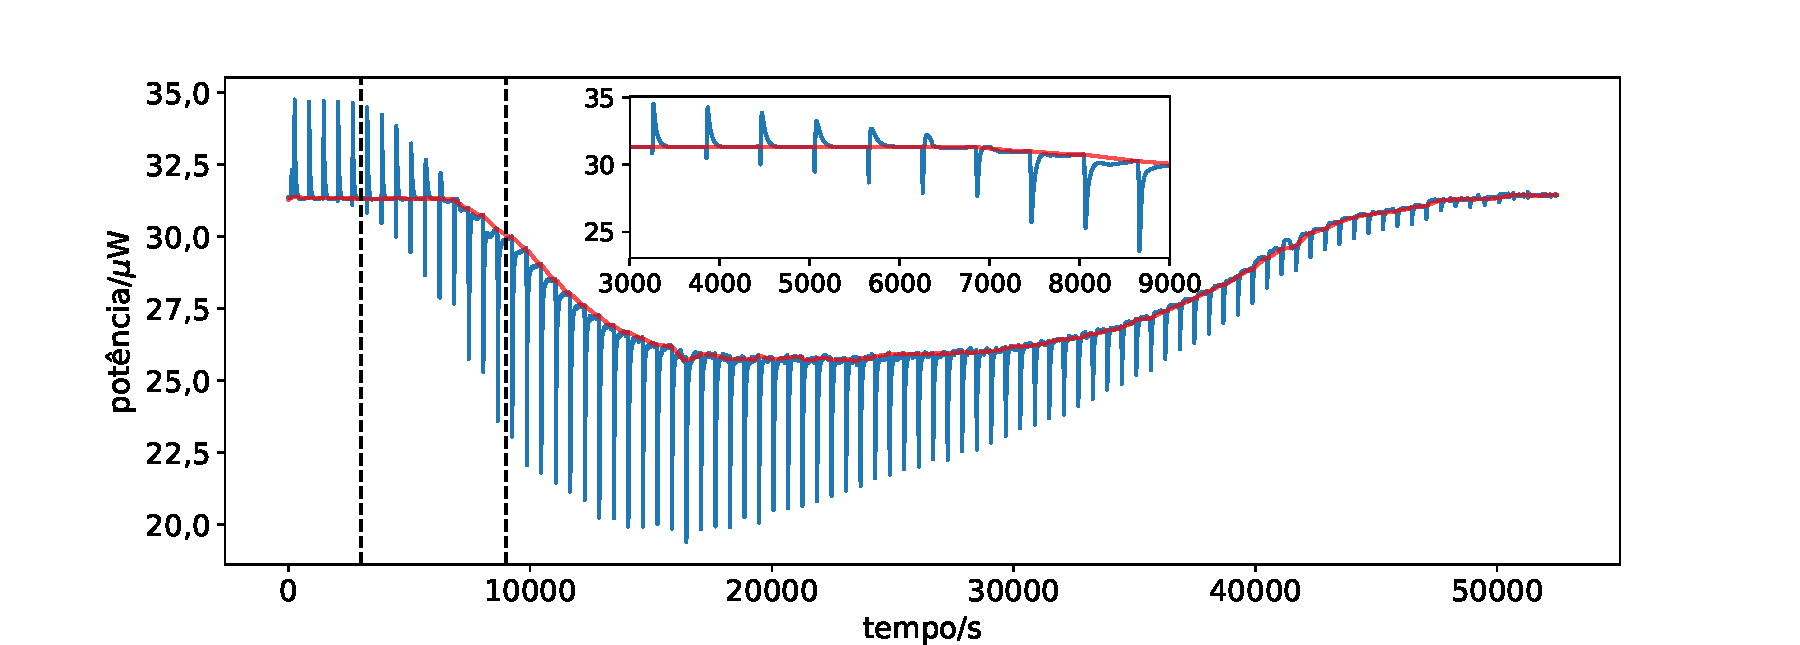
\includegraphics[width=\textwidth]{imagens/itc/exemplo_raw_mg}
				\caption{\TTAB{} 14 \mM em NaSal 1,5\mM. Solvente: água}
				\label{fig:itc_raw_mg}
			\end{subfigure}
		
			\begin{subfigure}{\textwidth}
				\centering
				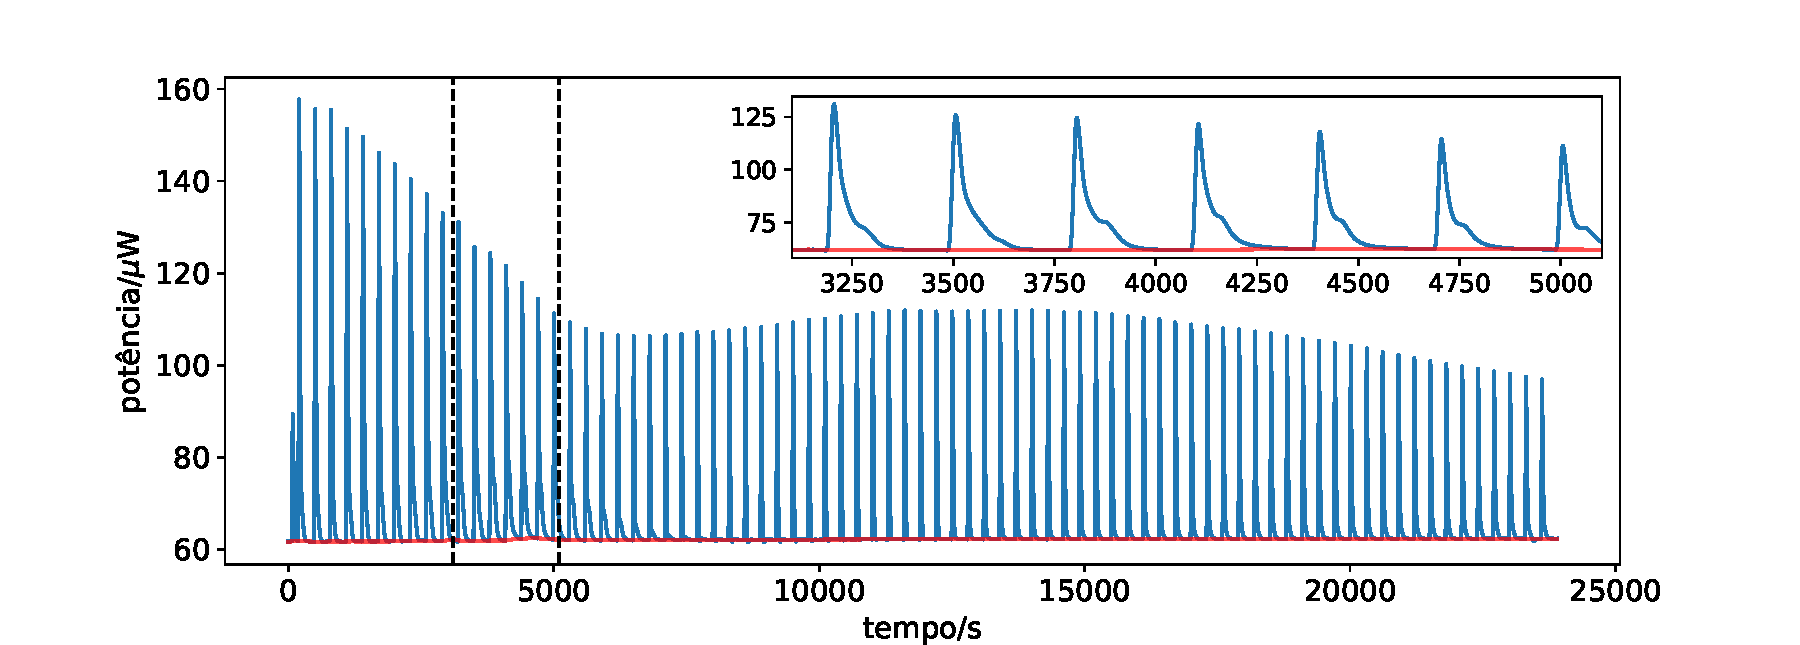
\includegraphics[width=\textwidth]{imagens/itc/raw_itc_glicerina}
				\caption{\TTAB{} 50 \mM em NaSal 1,5\mM. Solvente: glicerina 40\%}
				\label{fig:raw_itc_mg_glicerina}
			\end{subfigure}
			
			\caption{Potência necessária para manter a cela de amostra e de referência com a mesma temperatura durante uma titulação de \TTAB{} em NaSal 1,5 \mM{} em água e em glicerina 40\% m/m. A região onde se inicia a formação de micelas gigantes, marcada pelas retas verticais, está no \emph{inset}, mostrando a presença de dois picos. A linha vermelha é a linha de base criada pelo software.}
			\label{fig:itc_raw_agua_glicerina}
		\end{figure}
	
		O entalpograma integrado, \autoref{fig:itc_integrado_mg} possui um perfil semelhante a todos os sistemas de micelas gigantes estudados até agora, e inclusive foi chamado de ``assinatura'' da formação de micelas gigantes. \cite{Ito2016}
		\index{micelas gigantes!entalpograma}
		Esse entalpograma integrado foi tipicamente dividido em quatro regiões. Em concentrações pequenas de \TTAB, fo iproposto que ocorre a formação de micelas mistas, esféricas ou cilíndricas curtas. Em seguida, ocorre a fusão das micelas, liberando a energia de excesso das pontas (\autoref{eqn:distribuicao_tamanho_MG}), que leva à queda brusca nos valores de \(\Delta H\). Com a adição de mais \TTAB, o sistema sai da proporção ideal entre as espécies, e as micelas começam a encurtar até que, em grande excesso de \TTAB, as micelas se tornam esféricas, e a adição de mais \TTAB{} leva somente à diluição do conteúdo da seringa, e os valores de entalpia se aproximam de zero.\cite{Shukla2008, Ito2015c}
		
		Do entalpograma é possível obter a concentração de formação de micelas gigantes, \cwlm, e a entalpia de formação de micelas gigantes, \DHwlm. A posição de formação de micelas gigantes, \cwlm, não foi definida no ponto de inflexão, pois o máximo de viscosidade para os sistemas \TTAB{} e NaSal se encontra no ponto mínimo. \cite{Ito2015c}
		\index{micelas gigantes!\cwlm}
		% figura com esses parâmetros
		
		\begin{figure}[h]
			\centering
			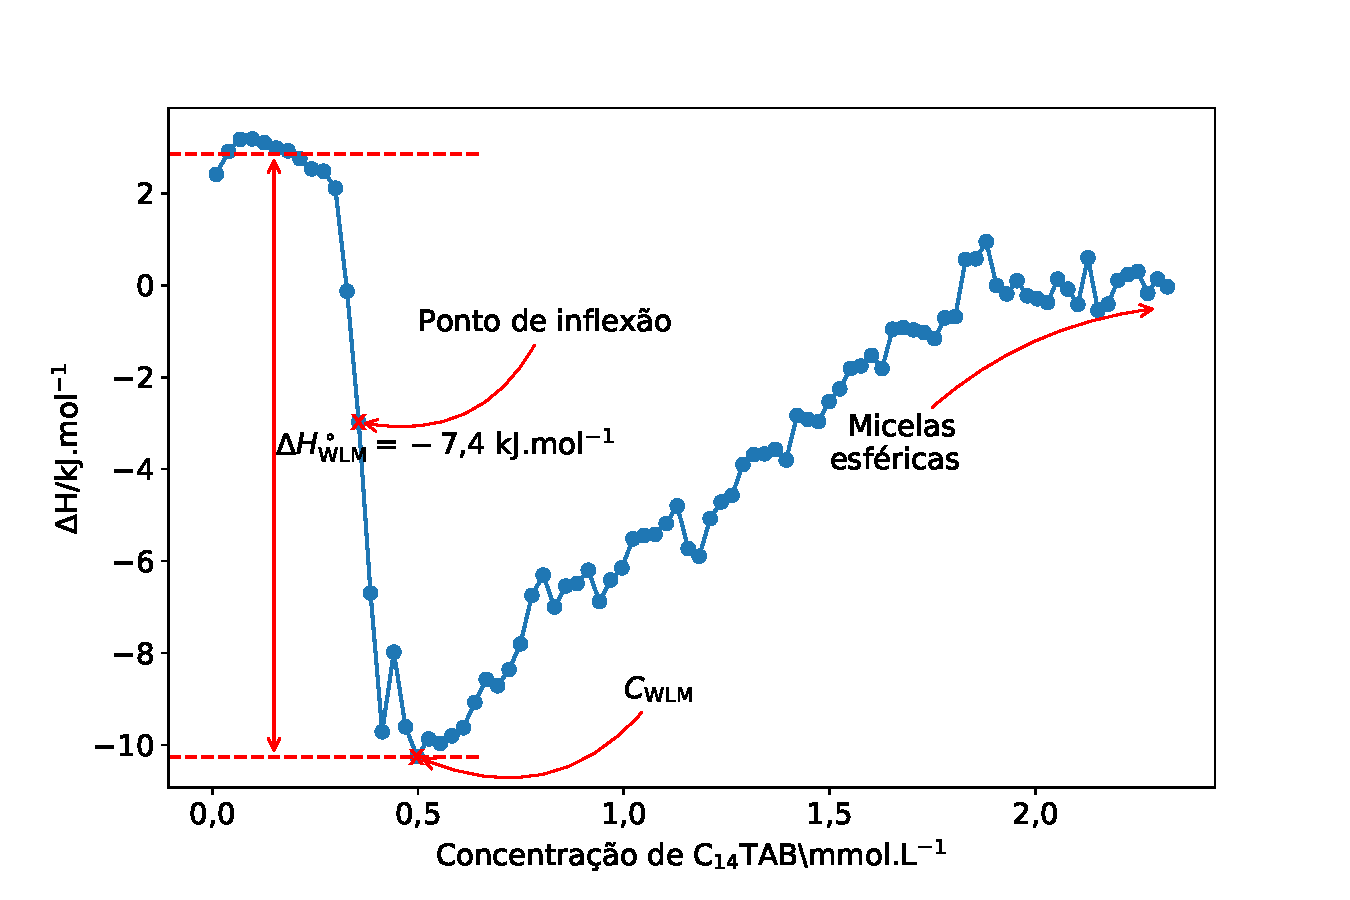
\includegraphics[width=0.7\textwidth]{imagens/itc/exemplo_integrado_mg}
			\caption{Potência integrada da \autoref{fig:itc_raw_mg}, resultando no entalpograma característico da formação de micelas gigantes. A concentração de formação de micelas gigantes \cwlm{} está definida, assim como a entalpia de micelização, \DHwlm.}
			\label{fig:itc_integrado_mg}
		\end{figure}
		
		\index{micelas gigantes!fluorescência}
		Resultados recentes do grupo, baseados nos experimentos de fluorescência apresentados neste trabalho, de tensão superficial e de fluorescência resolvida no tempo (na escala de ps), mostraram que essa interpretação está parcialmente equivocada. A região com baixa concentração de \TTAB{} não contém micelas esféricas ou cilíndricas curtas, e o início da incorporação de NaSal se inicia perto do ponto de inflexão. Nesse ponto, o \Sal{} e os monômeros de \TTAB{} começam a se juntar, formando micelas alongadas com carga negativa, que rapidamente se neutraliza quando a concentração de \TTAB{} é igual a \cwlm, onde a viscosidade e, consequentemente, o comprimento das micelas é máximo. A tendência de não formar micelas cilíndricas curtas se deve à energia de excesso das pontas, que seria grande demais, em comparação com a energia do corpo. Quando há surfactante suficiente para formar micelas mais compridas, diminuindo a penalidade das pontas, o processo de autoassociação ocorre. % todo: ref desse artigo, se sair a tempo
		
		\index{micelas gigantes!maneiras alternativas para experimentos de calorimetria}
		Outra maneira de se observar a autoassociação de micelas gigantes é titulando uma solução do cossoluto em uma solução de surfactante. Esse processo se aproximaria mais do procedimento utilizado para construir os diagramas de viscosidade da \autoref{fig:regioes_rh}.	A \autoref{fig:itc_inverso_normal_bases} mostra experimentos onde foram realizadas titulações de \TTAB{} em NaSal e de NaSal em \TTAB{}. Nos experimentos, a concentração do titulante foi fixada em 7,58 \mM{} e do titulado 1,50 \mM{}, de modo que, no final, a concentração das espécies seja 1,25 \mM{}, logo, o estado final dos dois processos é o mesmo. Note, no entanto, que no processo de adição de NaSal ao \TTAB, como já existem micelas de \TTAB, é esperado que ocorra a formação de micelas mistas antes da formação de micelas gigantes.
		
		Um problema com esse tipo de análise é determinar como exibir esse tipo de dado. É possível tanto utilizar a concentração de \TTAB{} quanto de NaSal na abscissa, mas isso acaba comprimindo um dos entalpogramas. Outra maneira é utilizar a concentração do titulado, porém, claramente, a abscissa possui significados diferentes. Esse tipo de experimento foi muito pouco estudado, e a definição de parâmetros como \cwlm{} ficam difíceis de serem definidas. Algumas questões pode ser levantadas. Por exemplo, caso a agregação seja observada em determinada concentração de NaSal, a concentração de \TTAB{} nesse ponto seria definida como sua \cwlm{} para tal concentração de NaSal? Estudos mais aprofundados, de viscosimetria e espalhamento de luz, dentre outras técnicas, são necessários para definir essa área.
		
		\begin{figure}
			\centering
			\begin{subfigure}{0.3\textwidth}
				\centering
				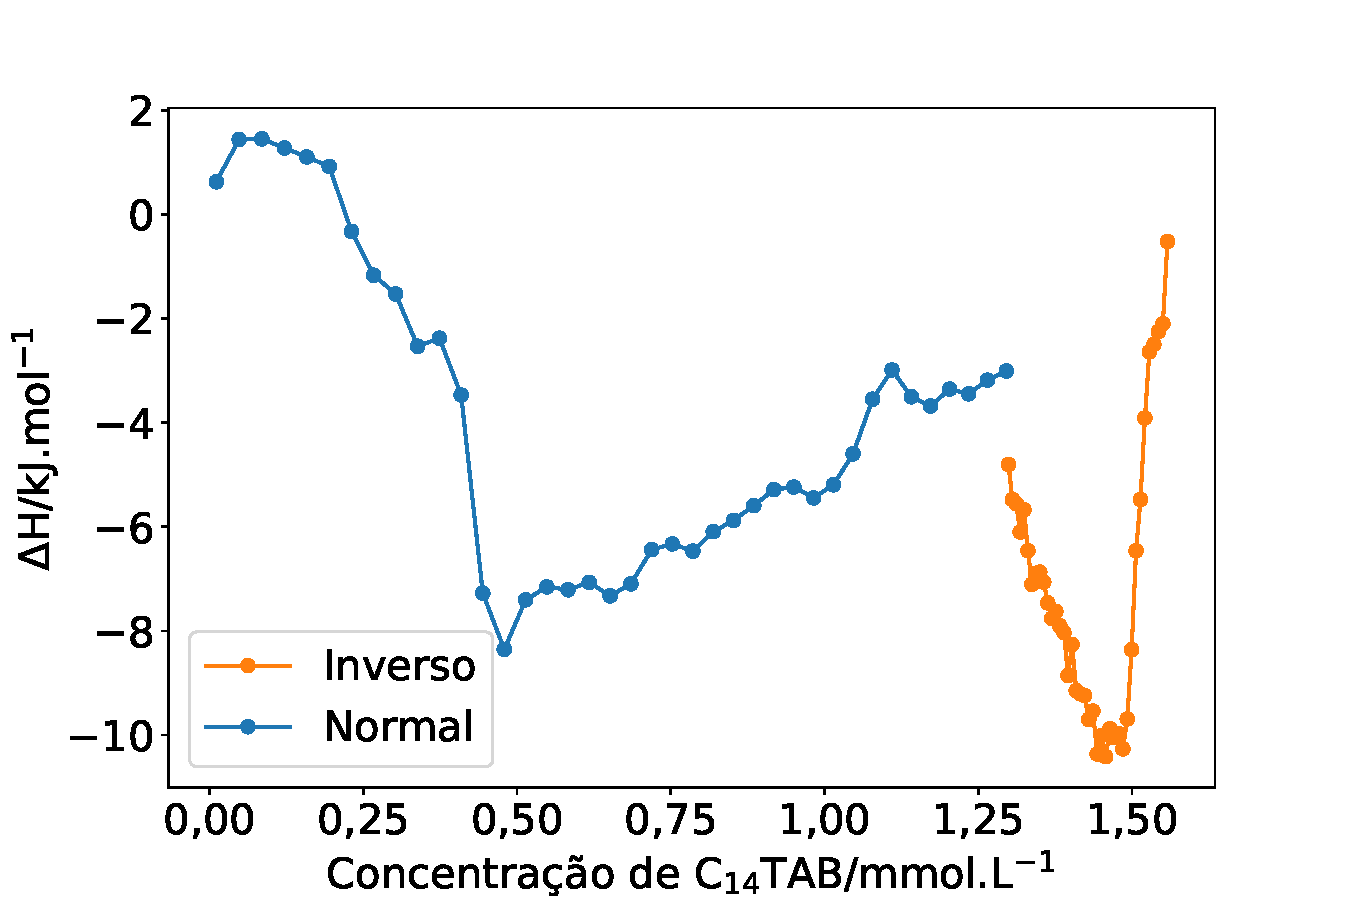
\includegraphics[width=\linewidth]{imagens/itc/itc_inverso_normal_base_ttab}
				\caption{\TTAB{}}
				\label{fig:itc_inverso_normal_base_ttab}
			\end{subfigure} %
			\begin{subfigure}{0.3\textwidth}
				\centering
				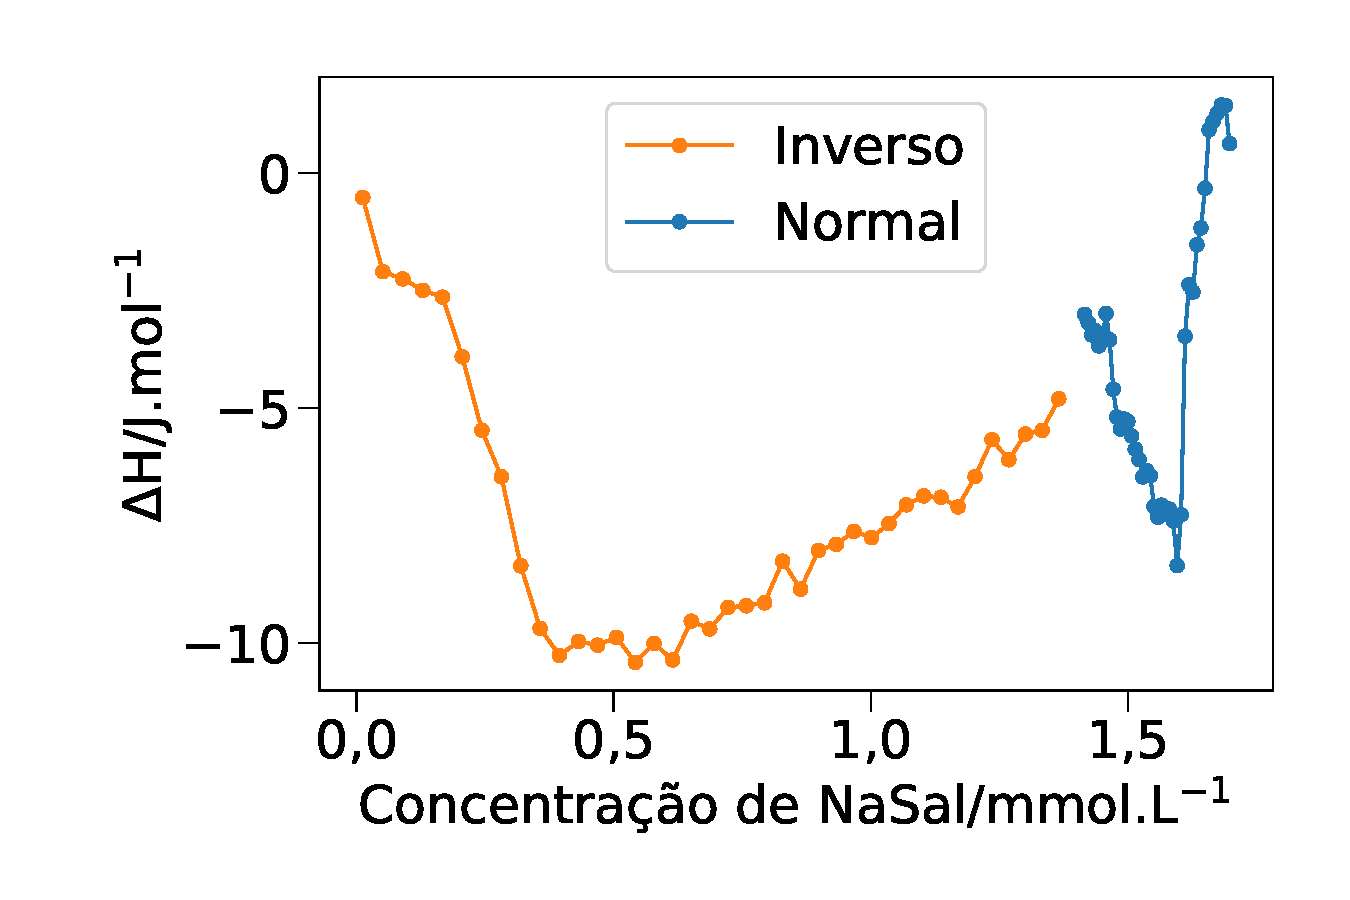
\includegraphics[width=\linewidth]{imagens/itc/itc_inverso_normal_base_nasal}
				\caption{NaSal}
				\label{fig:itc_inverso_normal_base_nasal}
			\end{subfigure} %
			\begin{subfigure}{0.3\textwidth}
				\centering
				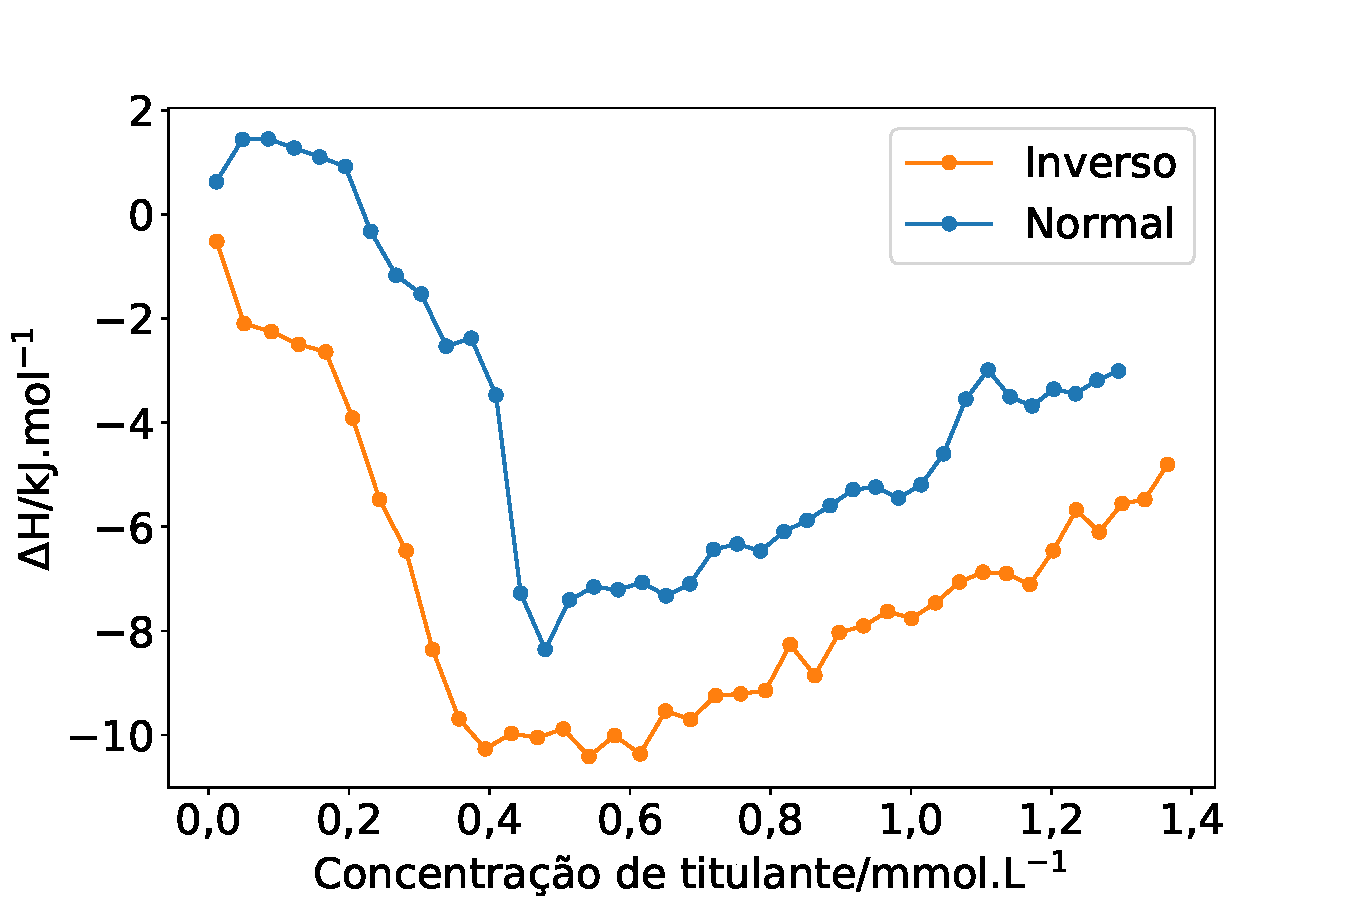
\includegraphics[width=\linewidth]{imagens/itc/itc_inverso_normal_basecomum}
				\caption{Titulante}
				\label{fig:itc_inverso_normal_basecomum}
			\end{subfigure}
			\caption{Entalpogramas de titulações de \TTAB{} 7,58 \mM{} em NaSal 1,5 \mM{}, e de NaSal 7,58 \mM{} em \TTAB{} 1,5 \mM{}. Três valores diferentes para a abscissa foram selecionados. \ref{fig:itc_inverso_normal_base_ttab}:concentração de \TTAB{} na cela. \ref{fig:itc_inverso_normal_base_nasal}: concentração de NaSal na cela. \ref{fig:itc_inverso_normal_basecomum}: concentração de titulante na cela}
			\label{fig:itc_inverso_normal_bases}
		\end{figure}
			
		Uma terceira maneira de se estudar a formação de micelas gigantes é titulando uma solução de micelas gigantes em água. Esse tipo de experimento também não foi muito aprofundado. Possivelmente, forneceria um segundo valor para a concentração de formação de micelas gigantes em determinada proporção de surfactante e cossoluto. A \autoref{fig:mg_em_agua} mostra dois experimentos de titulação de micelas gigantes nas proporções de 10:10 e 20:20 em água.

		\begin{figure}[h]
			\centering
			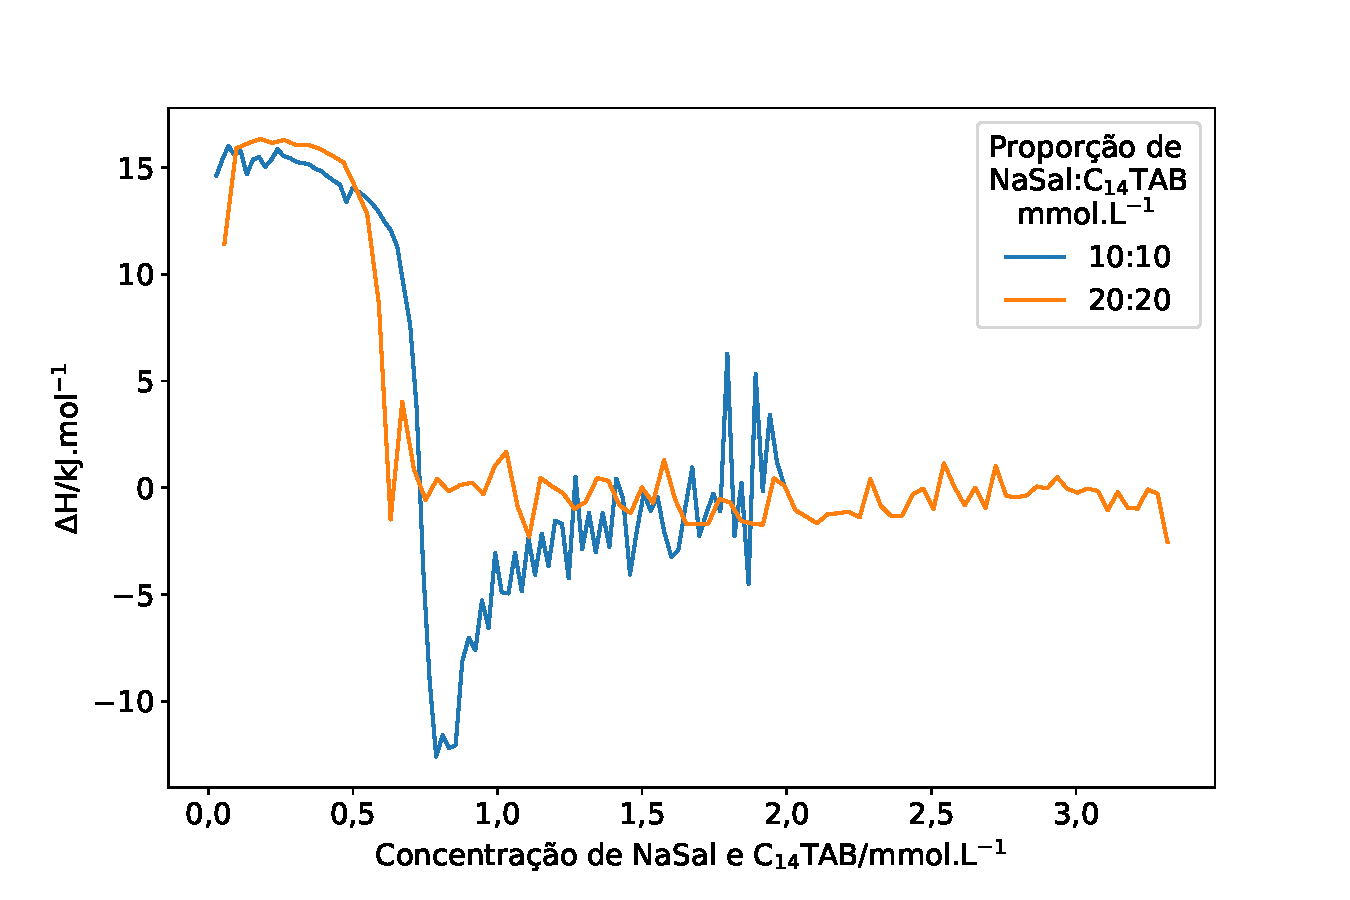
\includegraphics[width=0.7\textwidth]{imagens/itc/MG_em_agua}
			\caption{Entalpogramas de titulações de soluções com micelas gigantes de NaSal e \TTAB{}, equimolares, nas concentrações de 10 e 20 \mM.}
			\label{fig:mg_em_agua}
		\end{figure}

		\FloatBarrier

		\section{Efeito do solvente} \index{micelas gigantes!efeito do solvente}
		\label{sec:efeito_solvente}
		
		Hoffmann observou\cite{Grabner2014, Song2008a, Shinto2012} que a formação de lamelas não era afetada pela adição de alguns aditivos ao solvente, porém a distância interlamelar aumentava significativamente. A interpretação de Hoffmann para o intumescimento se baseou no índice de refração (\(n\)) do surfactante e do solvente, propriedades importantes para descrever a atração coloidal, como visto pela constante de Hamaker, \autoref{eqn:constante_hamaker_lifshitz}.
		\index{micelas gigantes!constante de Hamaker}
		
		Quando a concentração de glicerina em água atinge 60\% v/v, o índice de refração do solvente \(n_3\) e do agregado \(n_1\) se tornam iguais. Nessa situação, a atração interlamelar diminui muito, pois a constante de Hamaker, proporcional à diferença desses índices de refração, torna-se próxima de zero. Com a atração interlamelar anulada, as forças repulsivas de ondulação das lamelas conseguem separá-las, intumescendo o sistema.
		\index{micelas gigantes!índice de refração}
		
		Os sistemas estudados foram: 
		
		\begin{enumerate}[noitemsep]
			\item \citeauthor{Grabner2014}: diacilfosfatidilcolina com glicerina, 1,3-butanodiol, 1,2-propanodiol
			\item \citeauthor{Song2008a}: uma mistura de 5\% de um surfactante não iônico Genapol 070 (LA070) com 50\mM{} de octanol em DMSO, glicerina e sacarose (referenciada simplesmente como \emph{sugar}), e lecitina com glicerol
			\item \citeauthor{Shinto2012}: diacilfosfatifilcolina com água e glicerina.
		\end{enumerate}
		
		% todo: colocar uma lista de sistemas que o Hoffmann observou, para MG 
		
		\index{micelas gigantes!glicerina}
		
		Posteriormente, \citeauthor{Hoffmann2010} estudaram o efeito do solvente, utilizando glicerina, porém em micelas gigantes de \CTAB{} e NaSal. Observaram que havia uma grande diminuição na viscosidade dos dois picos de viscosidade, mas a região central, de mínimo de viscosidade, era pouco afetada. Nas regiões afetadas, a relaxação micelar ocorre principalmente por meio da reptação, e como a atração intermicelar se torna menor, devido à constante de Hamaker ser próxima de zero, as micelas conseguem reptar mais rapidamente, diminuindo a viscosidade. Na região central, onde o mecanismo principal é a quebra e recombinação, a atração intermicelar é pouco importante, portanto a viscosidade é pouco afetada. Maiores explicações para esse fenômeno podem ser encontradas na \autoref{sec:efeito_solvente}. 
		
		\index{micelas gigantes!1,3-butanodiol}
		Em seguida, \citeauthor{Abdel-Rahem2014} estudou o efeito do 1,3-butanodiol. Observou que a concentração de 1,3-butanodiol necessário para resultar numa queda de viscosidade é muito menor que glicerina, nas mesmas condições de índice de refração. Isso informa que considerar somente as interações intermicelares não é suficiente para explicar o efeito do aditivo. O autor levanta a hipótese que há um efeito adicional que está alterando o comportamento, a constante dielétrica, que afeta as interações eletrostáticas no meio. Ambos os parâmetros afetam os mecanismos de relaxação estrutural das micelas, alterando os tempos de relaxação e, consequentemente, as viscosidades. \index{micelas gigantes!constante dielétrica}
		
		% Falar sobre a hidrofilicidade da superfície micelar, o t3 de relaxação e a relação com os perfis de viscosidade.
		
		\index{micelas gigantes!sticky contacts@\textsl{sticky contacts}}
		Hoffmann também, em correspondências pessoais, mencionou que conseguiu observar um tempo de relaxação adicional por birrefringência elétrica\cite{Hoffmann1990} que estariam relacionados ao tempo em que as micelas demoram para tocar umas às outras. Esse processo, determinado como ``sticky contact''\cite{Hoffmann2010, Hoffmann2012a, Yamashita2006}, promove a maior viscosidade para sistemas com \CTAB{} do que com, por exemplo, C\textsubscript{16}PyCl, e estaria relacionado à hidrofilicidade da superfície micelar. Logo, micelas gigantes com superfícies mais hidrofílicas passariam menos tempo em contato, e os processos de relaxação seriam mais rápidos. 
		


		\chapter{Inspirações para o projeto} \index{micelas gigantes!inspirações}

		Os estudos de Hoffmann inspiraram grande parte deste trabalho, devido à correlação entre parâmetros macroscópicos do solvente com as propriedades reológicas das micelas gigantes. O fato de que é possível modular a viscosidade das micelas, mantendo sua estrutura, pela adição de glicerina, resultou em vários questionamentos e conversas durante a visita de Hoffmann ao grupo. Logo depois, decidiu-se continuar esses estudos, expandindo-os utilizando outros aditivos.
		
		Além disso, notou-se que haviam resultados de ITC (\autoref{fig:itc_raw_agua_glicerina}) que indicavam que poderiam existir dois processos ocorrendo em cada injeção, devido à existência de dois picos. A cinética desse processo era bastante longa. Além disso, esses processos cinéticos lentos ocorriam na região de formação de micelas gigantes. Começou-se a buscar técnicas para a determinação da cinética de crescimento.
		
		Pedersen, em uma série de artigos\cite{Jensen2013a, Jensen2014a, Jensen2016a}, observou o crescimento de micelas alongadas utilizando espalhamento de raios-X em baixos ângulos (SAXS), resolvido no tempo. Para iniciar o crescimento das micelas, foi utilizado um aparato de \emph{stopped-flow}, onde duas soluções, que não continham micelas gigantes, eram misturadas. Enquanto o sistema se dirigia ao equilíbrio, as micelas eram formadas. Dessa maneira, uma colaboração foi firmada com seu grupo, e foram medidas a cinética de crescimento. \index{micelas gigantes!cinética} \index{micelas gigantes!stopped-flow@\textsl{stopped-flow}}
		
		Em paralelo, observou-se que a fluorescência do salicilato se alterava dependendo da concentração de surfactante no meio. Caso esse processo de inserção e crescimento fosse lento o suficiente, seria possível observá-lo por fluorescência resolvida no tempo, mas em escalas de ms, ao invés de ps dos experimentos tradicionais desse ramo. Assim, o mesmo fenômeno seria observado, em paralelo, por duas técnicas diferentes.
			
	\chapter{Objetivos}
		Os objetivos deste projeto são:
		
		\begin{itemize}[noitemsep]
			\item Estudar como o solvente afeta a reologia de micelas gigantes de \CTAB{} e NaSal.
			\begin{itemize}[noitemsep]
				\item Variar a concentração de NaSal e observar como a viscosidade no repouso, \(\eta_0\), o módulo no platô \(G\), tempo de relaxação \(\tau_{\mathrm{rel}}\), e outros parâmetros, se comportam à medida que mais aditivo é adicionado à água.
				\begin{itemize}[noitemsep]
					\item Aditivos: Glicerina, sacarose, dimetilsulfóxido, 1,3-butanodiol, ureia.
					\item Concentrações: 0-60\% \(m_{\mathrm{aditivo}}/\left(m_{\mathrm{aditivo}}+m_{\mathrm{água}}\right)\), dependendo do aditivo.
				\end{itemize}
				\item Utilizar a teoria vigente na literatura para explicar o efeito do solvente, baseando-se na utilização de parâmetros macroscópicos, como índice de refração e constante dielétrica.
				\item Propor novos fatores para complementar a teoria vigente, caso seja necessário.
			\end{itemize}
			\item Estudar como o solvente afeta a formação de micelas gigantes de \TTAB{} e NaSal, através de calorimetria de titulação isotérmica. Os aditivos são os mesmos estudados para reologia.
			\begin{itemize}[noitemsep]
				\item Titular \TTAB{} em NaSal 1,5\mM{} em soluções com concentrações crescentes de aditivo em água.
				\item Titular \TTAB{} nas mesmas misturas binárias, sem NaSal.
				\item Comparar os resultados calorimétricos entre si e correlacioná-los com as propriedades do solvente.
				\item Comparar os resultados calorimétricos com os resultados reológicos
			\end{itemize}
			\item Estudar a cinética de crescimento de micelas gigantes através de:
			\begin{itemize}[noitemsep]
				\item Espalhamento de raios-X em baixos ângulos resolvido no tempo. Extrair informações de tamanho pelo ajuste de um modelo apropriado.
				\item Fluorescência de NaSal resolvido no tempo. Extrair informações a partir da taxa de decaimento/crescimento de fluorescência.
			\end{itemize}
			\item Comparar os resultados de cinética com as informações disponíveis na literatura.
		\end{itemize}
		